\documentclass[twoside]{book}

% Packages required by doxygen
\usepackage{fixltx2e}
\usepackage{calc}
\usepackage{doxygen}
\usepackage[export]{adjustbox} % also loads graphicx
\usepackage{graphicx}
\usepackage[utf8]{inputenc}
\usepackage{makeidx}
\usepackage{multicol}
\usepackage{multirow}
\PassOptionsToPackage{warn}{textcomp}
\usepackage{textcomp}
\usepackage[nointegrals]{wasysym}
\usepackage[table]{xcolor}

% Font selection
\usepackage[T1]{fontenc}
\usepackage[scaled=.90]{helvet}
\usepackage{courier}
\usepackage{amssymb}
\usepackage{sectsty}
\renewcommand{\familydefault}{\sfdefault}
\allsectionsfont{%
  \fontseries{bc}\selectfont%
  \color{darkgray}%
}
\renewcommand{\DoxyLabelFont}{%
  \fontseries{bc}\selectfont%
  \color{darkgray}%
}
\newcommand{\+}{\discretionary{\mbox{\scriptsize$\hookleftarrow$}}{}{}}

% Page & text layout
\usepackage{geometry}
\geometry{%
  a4paper,%
  top=2.5cm,%
  bottom=2.5cm,%
  left=2.5cm,%
  right=2.5cm%
}
\tolerance=750
\hfuzz=15pt
\hbadness=750
\setlength{\emergencystretch}{15pt}
\setlength{\parindent}{0cm}
\setlength{\parskip}{3ex plus 2ex minus 2ex}
\makeatletter
\renewcommand{\paragraph}{%
  \@startsection{paragraph}{4}{0ex}{-1.0ex}{1.0ex}{%
    \normalfont\normalsize\bfseries\SS@parafont%
  }%
}
\renewcommand{\subparagraph}{%
  \@startsection{subparagraph}{5}{0ex}{-1.0ex}{1.0ex}{%
    \normalfont\normalsize\bfseries\SS@subparafont%
  }%
}
\makeatother

% Headers & footers
\usepackage{fancyhdr}
\pagestyle{fancyplain}
\fancyhead[LE]{\fancyplain{}{\bfseries\thepage}}
\fancyhead[CE]{\fancyplain{}{}}
\fancyhead[RE]{\fancyplain{}{\bfseries\leftmark}}
\fancyhead[LO]{\fancyplain{}{\bfseries\rightmark}}
\fancyhead[CO]{\fancyplain{}{}}
\fancyhead[RO]{\fancyplain{}{\bfseries\thepage}}
\fancyfoot[LE]{\fancyplain{}{}}
\fancyfoot[CE]{\fancyplain{}{}}
\fancyfoot[RE]{\fancyplain{}{\bfseries\scriptsize Generated by Doxygen }}
\fancyfoot[LO]{\fancyplain{}{\bfseries\scriptsize Generated by Doxygen }}
\fancyfoot[CO]{\fancyplain{}{}}
\fancyfoot[RO]{\fancyplain{}{}}
\renewcommand{\footrulewidth}{0.4pt}
\renewcommand{\chaptermark}[1]{%
  \markboth{#1}{}%
}
\renewcommand{\sectionmark}[1]{%
  \markright{\thesection\ #1}%
}

% Indices & bibliography
\usepackage{natbib}
\usepackage[titles]{tocloft}
\setcounter{tocdepth}{3}
\setcounter{secnumdepth}{5}
\makeindex

% Hyperlinks (required, but should be loaded last)
\usepackage{ifpdf}
\ifpdf
  \usepackage[pdftex,pagebackref=true]{hyperref}
\else
  \usepackage[ps2pdf,pagebackref=true]{hyperref}
\fi
\hypersetup{%
  colorlinks=true,%
  linkcolor=blue,%
  citecolor=blue,%
  unicode%
}

% Custom commands
\newcommand{\clearemptydoublepage}{%
  \newpage{\pagestyle{empty}\cleardoublepage}%
}

\usepackage{caption}
\captionsetup{labelsep=space,justification=centering,font={bf},singlelinecheck=off,skip=4pt,position=top}

%===== C O N T E N T S =====

\begin{document}

% Titlepage & ToC
\hypersetup{pageanchor=false,
             bookmarksnumbered=true,
             pdfencoding=unicode
            }
\pagenumbering{alph}
\begin{titlepage}
\vspace*{7cm}
\begin{center}%
{\Large Neonlicht }\\
\vspace*{1cm}
{\large Generated by Doxygen 1.8.12}\\
\end{center}
\end{titlepage}
\clearemptydoublepage
\pagenumbering{roman}
\tableofcontents
\clearemptydoublepage
\pagenumbering{arabic}
\hypersetup{pageanchor=true}

%--- Begin generated contents ---
\chapter{Neonlicht documentation}
\label{index}\hypertarget{index}{}\hypertarget{index_intro_sec}{}\section{Introduction}\label{index_intro_sec}
\hyperlink{classNeonlicht}{Neonlicht} is a synthesizer engine targeting the fast and easy creation of Sound\+Units (aka synthesizers and audio effects) that run on most Unix/\+Linux machines.

More specifically \hyperlink{classNeonlicht}{Neonlicht} is targeting the Raspberry 3 computer. As such it is optimized to be used with the low computing power of this machine.

I am aiming at using the engine as part of teaching students in the field of digital media. As such, I am trying to design a system, that is generally understandable, does not require to much of a prior knowledge in audio programming, but still offers enough flexibilty and power to create interesting and expressive musical instruments and audio effects. Using the Raspberry 3 is part of this approach. I want the software to be running on cheap hardware allowing students to experiment without the need of having access to expensive fruity systems.\hypertarget{index_install_sec}{}\section{Installation}\label{index_install_sec}
Installing \hyperlink{classNeonlicht}{Neonlicht} on your computer is done by taking the usual steps. The code is self contained, meaning all nessecary libraries are added to the source distribution of \hyperlink{classNeonlicht}{Neonlicht}.

In order to compile \hyperlink{classNeonlicht}{Neonlicht} you first compile the underlying libraries and, in a second step, compile \hyperlink{classNeonlicht}{Neonlicht} and the additional tools.

P\+L\+E\+A\+SE N\+O\+TE\+: Part of this documentation is in German ... Sorry for the inconvenience. I am working on it \+:)\hypertarget{index_step1}{}\subsection{Step 1\+: Compiling the libraries}\label{index_step1}
to be done ... 
\chapter{Hierarchical Index}
\section{Class Hierarchy}
This inheritance list is sorted roughly, but not completely, alphabetically\+:\begin{DoxyCompactList}
\item \contentsline{section}{Activator}{\pageref{classActivator}}{}
\begin{DoxyCompactList}
\item \contentsline{section}{Osc\+Activator}{\pageref{classOscActivator}}{}
\end{DoxyCompactList}
\item \contentsline{section}{Central\+Store}{\pageref{classCentralStore}}{}
\item \contentsline{section}{Configuration\+Manager}{\pageref{classConfigurationManager}}{}
\item \contentsline{section}{Generic\+Queue$<$ T $>$}{\pageref{classGenericQueue}}{}
\item \contentsline{section}{Generic\+Queue$<$ osc\+:\+:Message\+Data $\ast$$>$}{\pageref{classGenericQueue}}{}
\item \contentsline{section}{Generic\+Queue$<$ Work\+Item $\ast$$>$}{\pageref{classGenericQueue}}{}
\item \contentsline{section}{Generic\+Thread}{\pageref{classGenericThread}}{}
\begin{DoxyCompactList}
\item \contentsline{section}{Consumer\+Thread}{\pageref{classConsumerThread}}{}
\end{DoxyCompactList}
\item \contentsline{section}{G\+UI}{\pageref{classGUI}}{}
\begin{DoxyCompactList}
\item \contentsline{section}{Workshop\+G\+UI}{\pageref{classWorkshopGUI}}{}
\end{DoxyCompactList}
\item \contentsline{section}{I\+D\+Generator}{\pageref{classIDGenerator}}{}
\item \contentsline{section}{Interpolation}{\pageref{classInterpolation}}{}
\item \contentsline{section}{util\+:\+:Key\+Pressed\+Control}{\pageref{classutil_1_1KeyPressedControl}}{}
\item \contentsline{section}{osc\+:\+:Message\+Data}{\pageref{classosc_1_1MessageData}}{}
\item \contentsline{section}{Message\+Data\+Queue}{\pageref{classMessageDataQueue}}{}
\item \contentsline{section}{osc\+:\+:Midi\+Connector}{\pageref{classosc_1_1MidiConnector}}{}
\item \contentsline{section}{util\+:\+:Midi\+Util}{\pageref{classutil_1_1MidiUtil}}{}
\item \contentsline{section}{Neonlicht}{\pageref{classNeonlicht}}{}
\item \contentsline{section}{osc\+:\+:Osc\+In\+Connector}{\pageref{classosc_1_1OscInConnector}}{}
\item \contentsline{section}{osc\+:\+:Osc\+Out\+Connector}{\pageref{classosc_1_1OscOutConnector}}{}
\item Osc\+Packet\+Listener\begin{DoxyCompactList}
\item \contentsline{section}{Example\+Packet\+Listener}{\pageref{classExamplePacketListener}}{}
\item \contentsline{section}{osc\+:\+:Osc\+In\+Connector\+:\+:Midi\+Packet\+Listener}{\pageref{classOscInConnector_1_1MidiPacketListener}}{}
\end{DoxyCompactList}
\item \contentsline{section}{Osc\+Wrapper}{\pageref{classOscWrapper}}{}
\item \contentsline{section}{Patch}{\pageref{classPatch}}{}
\item \contentsline{section}{Port}{\pageref{classPort}}{}
\item \contentsline{section}{Pulse}{\pageref{classPulse}}{}
\item \contentsline{section}{Test\+Static}{\pageref{classTestStatic}}{}
\item \contentsline{section}{Tick\+Data}{\pageref{structTickData}}{}
\item \contentsline{section}{unit\+:\+:U\+Gen}{\pageref{classunit_1_1UGen}}{}
\begin{DoxyCompactList}
\item \contentsline{section}{unit\+:\+:Add\+Two\+Gen}{\pageref{classunit_1_1AddTwoGen}}{}
\item \contentsline{section}{unit\+:\+:Envelope\+Gen}{\pageref{classunit_1_1EnvelopeGen}}{}
\begin{DoxyCompactList}
\item \contentsline{section}{unit\+:\+:A\+D\+S\+R\+Gen}{\pageref{classunit_1_1ADSRGen}}{}
\item \contentsline{section}{unit\+:\+:E\+G\+One\+Step\+Gen}{\pageref{classunit_1_1EGOneStepGen}}{}
\item \contentsline{section}{unit\+:\+:E\+G\+Up\+Down\+Gen}{\pageref{classunit_1_1EGUpDownGen}}{}
\end{DoxyCompactList}
\item \contentsline{section}{unit\+:\+:Gated\+Constant\+Gen}{\pageref{classunit_1_1GatedConstantGen}}{}
\item \contentsline{section}{unit\+:\+:Invert\+Gen}{\pageref{classunit_1_1InvertGen}}{}
\item \contentsline{section}{unit\+:\+:Midi\+Input\+Gen}{\pageref{classunit_1_1MidiInputGen}}{}
\item \contentsline{section}{unit\+:\+:Multiply\+Gen}{\pageref{classunit_1_1MultiplyGen}}{}
\item \contentsline{section}{unit\+:\+:Multiply\+Two\+Gen}{\pageref{classunit_1_1MultiplyTwoGen}}{}
\item \contentsline{section}{unit\+:\+:Multi\+Switch5\+Gen}{\pageref{classunit_1_1MultiSwitch5Gen}}{}
\item \contentsline{section}{unit\+:\+:Number\+Gen}{\pageref{classunit_1_1NumberGen}}{}
\item \contentsline{section}{unit\+:\+:One\+Pole\+L\+P\+F\+Gen}{\pageref{classunit_1_1OnePoleLPFGen}}{}
\item \contentsline{section}{unit\+:\+:Oscillator\+Gen}{\pageref{classunit_1_1OscillatorGen}}{}
\begin{DoxyCompactList}
\item \contentsline{section}{unit\+:\+:Noise\+Gen}{\pageref{classunit_1_1NoiseGen}}{}
\item \contentsline{section}{unit\+:\+:Saw\+Gen}{\pageref{classunit_1_1SawGen}}{}
\begin{DoxyCompactList}
\item \contentsline{section}{unit\+:\+:Cosine\+Gen}{\pageref{classunit_1_1CosineGen}}{}
\begin{DoxyCompactList}
\item \contentsline{section}{unit\+:\+:Pulse\+Gen}{\pageref{classunit_1_1PulseGen}}{}
\begin{DoxyCompactList}
\item \contentsline{section}{unit\+:\+:Square\+Gen}{\pageref{classunit_1_1SquareGen}}{}
\end{DoxyCompactList}
\end{DoxyCompactList}
\item \contentsline{section}{unit\+:\+:Phasor\+Gen}{\pageref{classunit_1_1PhasorGen}}{}
\end{DoxyCompactList}
\end{DoxyCompactList}
\item \contentsline{section}{unit\+:\+:Sound\+Unit}{\pageref{classunit_1_1SoundUnit}}{}
\begin{DoxyCompactList}
\item \contentsline{section}{Arturia\+Mini\+Lab\+Unit}{\pageref{classArturiaMiniLabUnit}}{}
\begin{DoxyCompactList}
\item \contentsline{section}{A\+D\+S\+R\+Workshop\+S\+PU}{\pageref{classADSRWorkshopSPU}}{}
\item \contentsline{section}{Multi\+Oscillator\+S\+PU}{\pageref{classMultiOscillatorSPU}}{}
\begin{DoxyCompactList}
\item \contentsline{section}{L\+F\+O\+Workshop\+S\+PU}{\pageref{classLFOWorkshopSPU}}{}
\end{DoxyCompactList}
\item \contentsline{section}{V\+C\+O\+Mod\+S\+PU}{\pageref{classVCOModSPU}}{}
\item \contentsline{section}{Workshop\+S\+PU}{\pageref{classWorkshopSPU}}{}
\end{DoxyCompactList}
\item \contentsline{section}{Noise\+Unit}{\pageref{classNoiseUnit}}{}
\end{DoxyCompactList}
\item \contentsline{section}{unit\+:\+:S\+T\+K\+Adapter\+Gen}{\pageref{classunit_1_1STKAdapterGen}}{}
\begin{DoxyCompactList}
\item \contentsline{section}{unit\+:\+:S\+T\+K\+Bi\+Quad\+Gen}{\pageref{classunit_1_1STKBiQuadGen}}{}
\item \contentsline{section}{unit\+:\+:S\+T\+K\+One\+Pole\+Gen}{\pageref{classunit_1_1STKOnePoleGen}}{}
\item \contentsline{section}{unit\+:\+:S\+T\+K\+One\+Zero\+Gen}{\pageref{classunit_1_1STKOneZeroGen}}{}
\item \contentsline{section}{unit\+:\+:S\+T\+K\+Two\+Pole\+Gen}{\pageref{classunit_1_1STKTwoPoleGen}}{}
\item \contentsline{section}{unit\+:\+:S\+T\+K\+Two\+Zero\+Gen}{\pageref{classunit_1_1STKTwoZeroGen}}{}
\end{DoxyCompactList}
\item \contentsline{section}{unit\+:\+:Threshold\+Gen}{\pageref{classunit_1_1ThresholdGen}}{}
\item \contentsline{section}{unit\+:\+:Two\+Input\+Mixer\+Gen}{\pageref{classunit_1_1TwoInputMixerGen}}{}
\item \contentsline{section}{unit\+:\+:Wave\+Out\+Gen}{\pageref{classunit_1_1WaveOutGen}}{}
\end{DoxyCompactList}
\item \contentsline{section}{Wave\+Table}{\pageref{classWaveTable}}{}
\begin{DoxyCompactList}
\item \contentsline{section}{Cosine\+Table}{\pageref{classCosineTable}}{}
\end{DoxyCompactList}
\item \contentsline{section}{Wave\+Writer}{\pageref{classWaveWriter}}{}
\item \contentsline{section}{Work\+Item}{\pageref{classWorkItem}}{}
\end{DoxyCompactList}

\chapter{Class Index}
\section{Class List}
Here are the classes, structs, unions and interfaces with brief descriptions\+:\begin{DoxyCompactList}
\item\contentsline{section}{\hyperlink{classActivator}{Activator} }{\pageref{classActivator}}{}
\item\contentsline{section}{\hyperlink{classunit_1_1AddTwoGen}{unit\+::\+Add\+Two\+Gen} }{\pageref{classunit_1_1AddTwoGen}}{}
\item\contentsline{section}{\hyperlink{classunit_1_1ADSRGen}{unit\+::\+A\+D\+S\+R\+Gen} }{\pageref{classunit_1_1ADSRGen}}{}
\item\contentsline{section}{\hyperlink{classCentralStore}{Central\+Store} }{\pageref{classCentralStore}}{}
\item\contentsline{section}{\hyperlink{classConfigurationManager}{Configuration\+Manager} }{\pageref{classConfigurationManager}}{}
\item\contentsline{section}{\hyperlink{classConsumerThread}{Consumer\+Thread} }{\pageref{classConsumerThread}}{}
\item\contentsline{section}{\hyperlink{classunit_1_1CosineGen}{unit\+::\+Cosine\+Gen} }{\pageref{classunit_1_1CosineGen}}{}
\item\contentsline{section}{\hyperlink{classCosineTable}{Cosine\+Table} }{\pageref{classCosineTable}}{}
\item\contentsline{section}{\hyperlink{classunit_1_1EGOneStepGen}{unit\+::\+E\+G\+One\+Step\+Gen} }{\pageref{classunit_1_1EGOneStepGen}}{}
\item\contentsline{section}{\hyperlink{classunit_1_1EGUpDownGen}{unit\+::\+E\+G\+Up\+Down\+Gen} }{\pageref{classunit_1_1EGUpDownGen}}{}
\item\contentsline{section}{\hyperlink{classExamplePacketListener}{Example\+Packet\+Listener} }{\pageref{classExamplePacketListener}}{}
\item\contentsline{section}{\hyperlink{classunit_1_1GatedConstantGen}{unit\+::\+Gated\+Constant\+Gen} }{\pageref{classunit_1_1GatedConstantGen}}{}
\item\contentsline{section}{\hyperlink{classGenericQueue}{Generic\+Queue$<$ T $>$} }{\pageref{classGenericQueue}}{}
\item\contentsline{section}{\hyperlink{classGenericThread}{Generic\+Thread} }{\pageref{classGenericThread}}{}
\item\contentsline{section}{\hyperlink{classIDGenerator}{I\+D\+Generator} }{\pageref{classIDGenerator}}{}
\item\contentsline{section}{\hyperlink{classInterpolation}{Interpolation} }{\pageref{classInterpolation}}{}
\item\contentsline{section}{\hyperlink{classutil_1_1KeyPressedControl}{util\+::\+Key\+Pressed\+Control} }{\pageref{classutil_1_1KeyPressedControl}}{}
\item\contentsline{section}{\hyperlink{classosc_1_1MessageData}{osc\+::\+Message\+Data} }{\pageref{classosc_1_1MessageData}}{}
\item\contentsline{section}{\hyperlink{classMessageDataQueue}{Message\+Data\+Queue} }{\pageref{classMessageDataQueue}}{}
\item\contentsline{section}{\hyperlink{classosc_1_1MidiConnector}{osc\+::\+Midi\+Connector} }{\pageref{classosc_1_1MidiConnector}}{}
\item\contentsline{section}{\hyperlink{classunit_1_1MidiInputGen}{unit\+::\+Midi\+Input\+Gen} }{\pageref{classunit_1_1MidiInputGen}}{}
\item\contentsline{section}{\hyperlink{classOscInConnector_1_1MidiPacketListener}{osc\+::\+Osc\+In\+Connector\+::\+Midi\+Packet\+Listener} }{\pageref{classOscInConnector_1_1MidiPacketListener}}{}
\item\contentsline{section}{\hyperlink{classunit_1_1MultiplyGen}{unit\+::\+Multiply\+Gen} }{\pageref{classunit_1_1MultiplyGen}}{}
\item\contentsline{section}{\hyperlink{classunit_1_1MultiplyTwoGen}{unit\+::\+Multiply\+Two\+Gen} }{\pageref{classunit_1_1MultiplyTwoGen}}{}
\item\contentsline{section}{\hyperlink{classNeonlicht}{Neonlicht} }{\pageref{classNeonlicht}}{}
\item\contentsline{section}{\hyperlink{classunit_1_1NoiseGen}{unit\+::\+Noise\+Gen} }{\pageref{classunit_1_1NoiseGen}}{}
\item\contentsline{section}{\hyperlink{classNoiseUnit}{Noise\+Unit} }{\pageref{classNoiseUnit}}{}
\item\contentsline{section}{\hyperlink{classunit_1_1NumberGen}{unit\+::\+Number\+Gen} }{\pageref{classunit_1_1NumberGen}}{}
\item\contentsline{section}{\hyperlink{classunit_1_1OnePoleLPFGen}{unit\+::\+One\+Pole\+L\+P\+F\+Gen} }{\pageref{classunit_1_1OnePoleLPFGen}}{}
\item\contentsline{section}{\hyperlink{classOscActivator}{Osc\+Activator} }{\pageref{classOscActivator}}{}
\item\contentsline{section}{\hyperlink{classosc_1_1OscInConnector}{osc\+::\+Osc\+In\+Connector} }{\pageref{classosc_1_1OscInConnector}}{}
\item\contentsline{section}{\hyperlink{classosc_1_1OscOutConnector}{osc\+::\+Osc\+Out\+Connector} }{\pageref{classosc_1_1OscOutConnector}}{}
\item\contentsline{section}{\hyperlink{classOscWrapper}{Osc\+Wrapper} }{\pageref{classOscWrapper}}{}
\item\contentsline{section}{\hyperlink{classPatch}{Patch} }{\pageref{classPatch}}{}
\item\contentsline{section}{\hyperlink{classunit_1_1PhasorGen}{unit\+::\+Phasor\+Gen} }{\pageref{classunit_1_1PhasorGen}}{}
\item\contentsline{section}{\hyperlink{classPort}{Port} }{\pageref{classPort}}{}
\item\contentsline{section}{\hyperlink{classPulse}{Pulse} }{\pageref{classPulse}}{}
\item\contentsline{section}{\hyperlink{classunit_1_1SawGen}{unit\+::\+Saw\+Gen} }{\pageref{classunit_1_1SawGen}}{}
\item\contentsline{section}{\hyperlink{classunit_1_1SoundUnit}{unit\+::\+Sound\+Unit} }{\pageref{classunit_1_1SoundUnit}}{}
\item\contentsline{section}{\hyperlink{classunit_1_1SquareGen}{unit\+::\+Square\+Gen} }{\pageref{classunit_1_1SquareGen}}{}
\item\contentsline{section}{\hyperlink{classunit_1_1STKAdapterGen}{unit\+::\+S\+T\+K\+Adapter\+Gen} }{\pageref{classunit_1_1STKAdapterGen}}{}
\item\contentsline{section}{\hyperlink{classunit_1_1STKBiQuadGen}{unit\+::\+S\+T\+K\+Bi\+Quad\+Gen} }{\pageref{classunit_1_1STKBiQuadGen}}{}
\item\contentsline{section}{\hyperlink{classunit_1_1STKOnePoleGen}{unit\+::\+S\+T\+K\+One\+Pole\+Gen} }{\pageref{classunit_1_1STKOnePoleGen}}{}
\item\contentsline{section}{\hyperlink{classunit_1_1STKOneZeroGen}{unit\+::\+S\+T\+K\+One\+Zero\+Gen} }{\pageref{classunit_1_1STKOneZeroGen}}{}
\item\contentsline{section}{\hyperlink{classunit_1_1STKTwoPoleGen}{unit\+::\+S\+T\+K\+Two\+Pole\+Gen} }{\pageref{classunit_1_1STKTwoPoleGen}}{}
\item\contentsline{section}{\hyperlink{classunit_1_1STKTwoZeroGen}{unit\+::\+S\+T\+K\+Two\+Zero\+Gen} }{\pageref{classunit_1_1STKTwoZeroGen}}{}
\item\contentsline{section}{\hyperlink{classTestStatic}{Test\+Static} }{\pageref{classTestStatic}}{}
\item\contentsline{section}{\hyperlink{classunit_1_1ThresholdGen}{unit\+::\+Threshold\+Gen} }{\pageref{classunit_1_1ThresholdGen}}{}
\item\contentsline{section}{\hyperlink{structTickData}{Tick\+Data} }{\pageref{structTickData}}{}
\item\contentsline{section}{\hyperlink{classunit_1_1TwoInputMixerGen}{unit\+::\+Two\+Input\+Mixer\+Gen} }{\pageref{classunit_1_1TwoInputMixerGen}}{}
\item\contentsline{section}{\hyperlink{classunit_1_1UGen}{unit\+::\+U\+Gen} }{\pageref{classunit_1_1UGen}}{}
\item\contentsline{section}{\hyperlink{classunit_1_1WaveOutGen}{unit\+::\+Wave\+Out\+Gen} }{\pageref{classunit_1_1WaveOutGen}}{}
\item\contentsline{section}{\hyperlink{classWaveTable}{Wave\+Table} }{\pageref{classWaveTable}}{}
\item\contentsline{section}{\hyperlink{classWaveWriter}{Wave\+Writer} }{\pageref{classWaveWriter}}{}
\item\contentsline{section}{\hyperlink{classWorkItem}{Work\+Item} }{\pageref{classWorkItem}}{}
\end{DoxyCompactList}

\chapter{Class Documentation}
\hypertarget{classActivator}{}\section{Activator Class Reference}
\label{classActivator}\index{Activator@{Activator}}
Inheritance diagram for Activator\+:\begin{figure}[H]
\begin{center}
\leavevmode
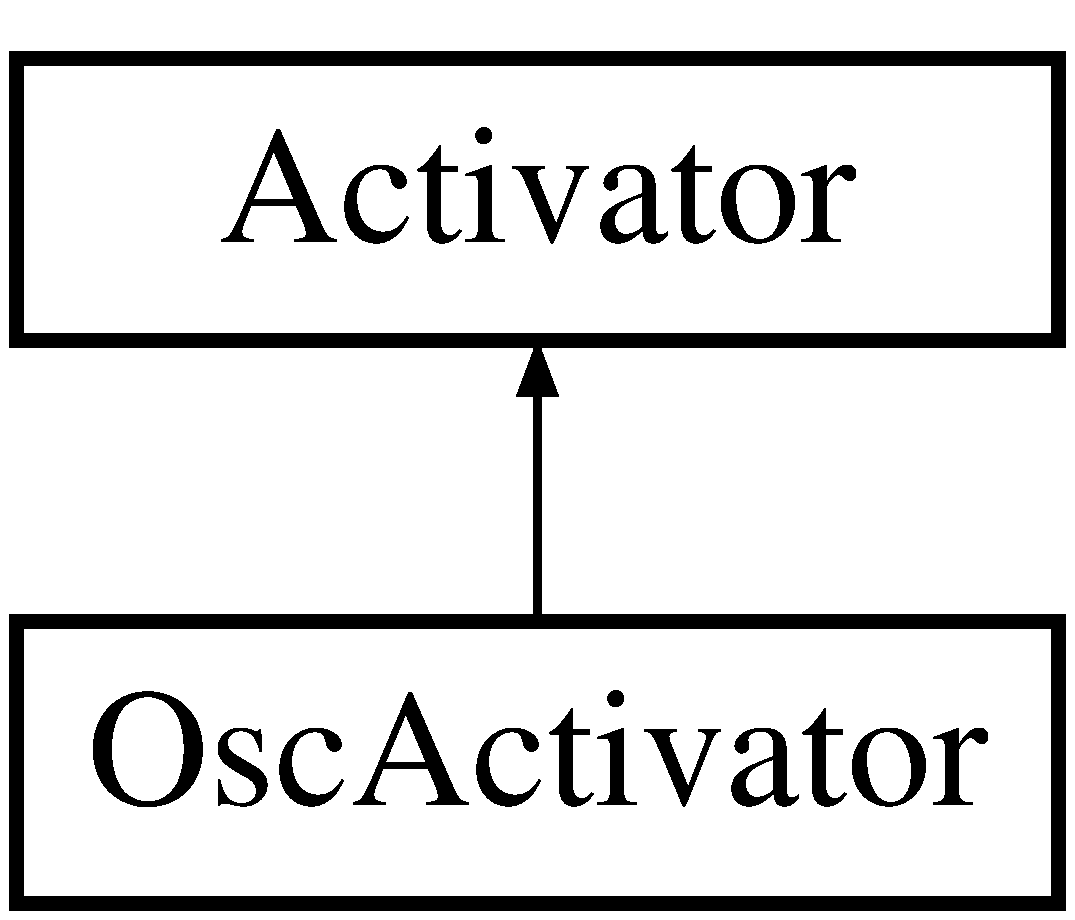
\includegraphics[height=2.000000cm]{classActivator}
\end{center}
\end{figure}
\subsection*{Public Member Functions}
\begin{DoxyCompactItemize}
\item 
virtual void {\bfseries callback} (float value)\hypertarget{classActivator_ace74b175ffcc2ad9cc03f15a0e713743}{}\label{classActivator_ace74b175ffcc2ad9cc03f15a0e713743}

\end{DoxyCompactItemize}


The documentation for this class was generated from the following files\+:\begin{DoxyCompactItemize}
\item 
include/Activator.\+h\item 
sequencer/Activator.\+cpp\end{DoxyCompactItemize}

\hypertarget{classAddTwoGen}{}\section{Add\+Two\+Gen Class Reference}
\label{classAddTwoGen}\index{Add\+Two\+Gen@{Add\+Two\+Gen}}
Inheritance diagram for Add\+Two\+Gen\+:\begin{figure}[H]
\begin{center}
\leavevmode
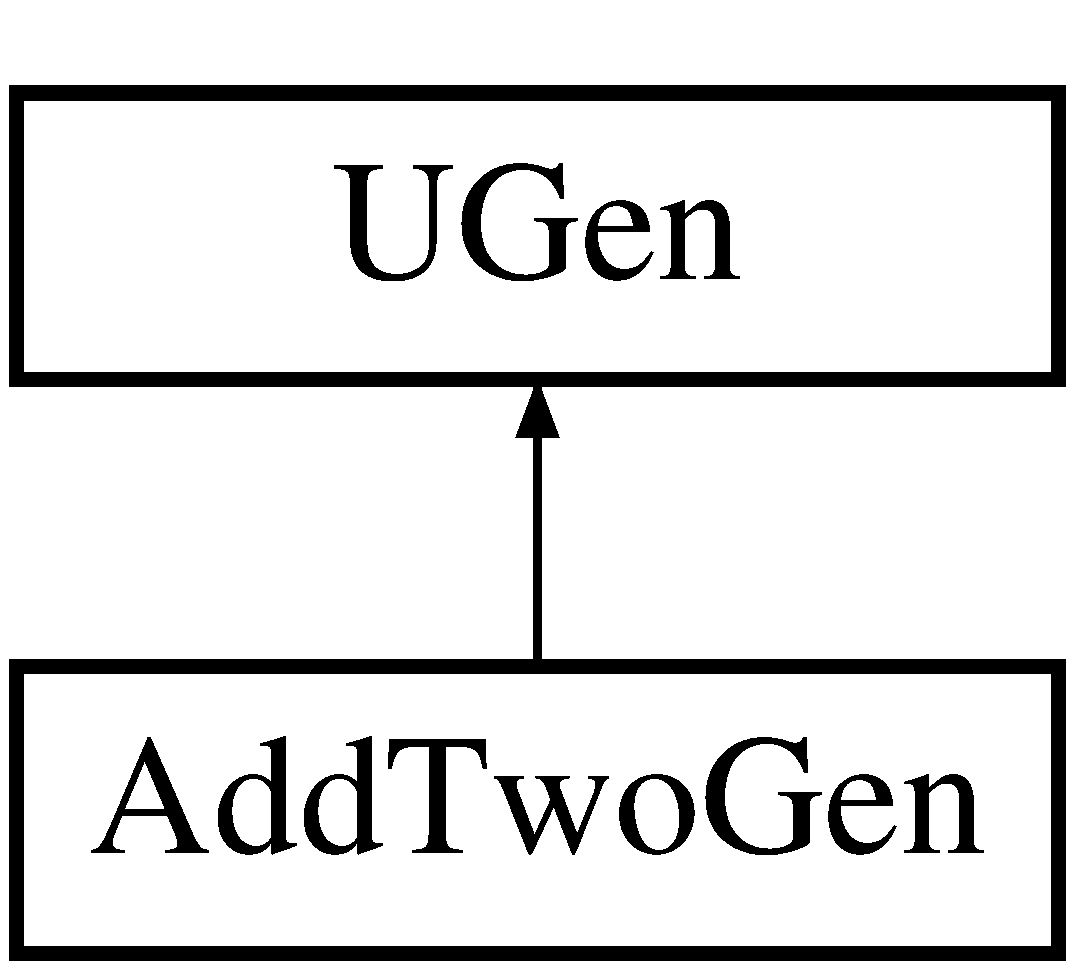
\includegraphics[height=2.000000cm]{classAddTwoGen}
\end{center}
\end{figure}
\subsection*{Public Member Functions}
\begin{DoxyCompactItemize}
\item 
{\bfseries Add\+Two\+Gen} (std\+::string name)\hypertarget{classAddTwoGen_a6feb4da948f12b37eb4502899b5a4311}{}\label{classAddTwoGen_a6feb4da948f12b37eb4502899b5a4311}

\item 
void {\bfseries control} (std\+::string port\+Name, float value)\hypertarget{classAddTwoGen_a5e0a82722566595b7284386a618ef3cb}{}\label{classAddTwoGen_a5e0a82722566595b7284386a618ef3cb}

\item 
float {\bfseries tick} ()\hypertarget{classAddTwoGen_a8e667f4f6c6849faef9f07a62e779d9a}{}\label{classAddTwoGen_a8e667f4f6c6849faef9f07a62e779d9a}

\end{DoxyCompactItemize}
\subsection*{Additional Inherited Members}


The documentation for this class was generated from the following files\+:\begin{DoxyCompactItemize}
\item 
unit/Add\+Two\+Gen.\+h\item 
unit/Add\+Two\+Gen.\+cpp\end{DoxyCompactItemize}

\hypertarget{classADSRGen}{}\section{A\+D\+S\+R\+Gen Class Reference}
\label{classADSRGen}\index{A\+D\+S\+R\+Gen@{A\+D\+S\+R\+Gen}}
Inheritance diagram for A\+D\+S\+R\+Gen\+:\begin{figure}[H]
\begin{center}
\leavevmode
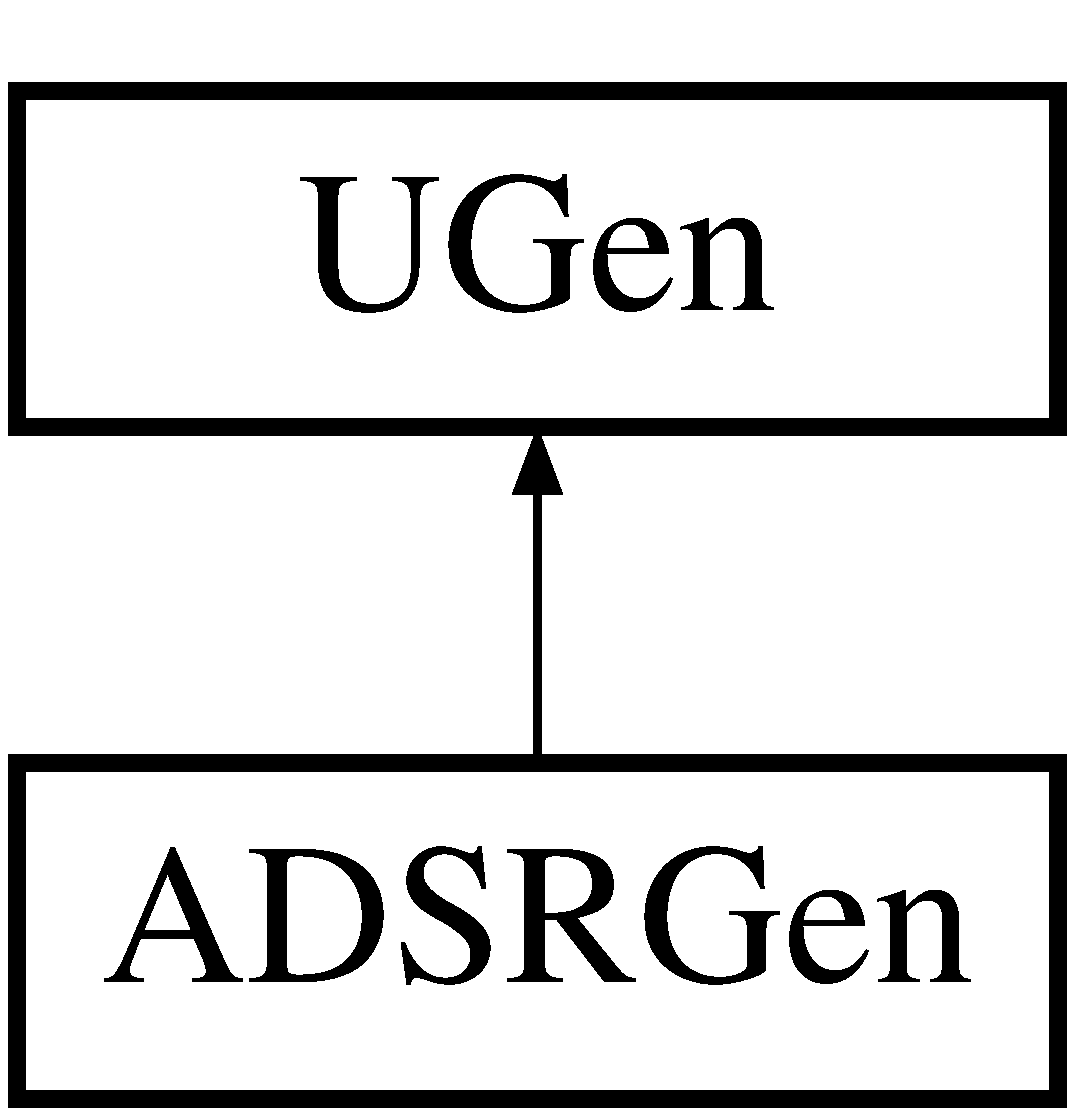
\includegraphics[height=2.000000cm]{classADSRGen}
\end{center}
\end{figure}
\subsection*{Public Member Functions}
\begin{DoxyCompactItemize}
\item 
{\bfseries A\+D\+S\+R\+Gen} (std\+::string name)\hypertarget{classADSRGen_a7e2d63eecbe51fc86a93697dd4d47964}{}\label{classADSRGen_a7e2d63eecbe51fc86a93697dd4d47964}

\item 
void {\bfseries control} (std\+::string port\+Name, float value)\hypertarget{classADSRGen_ac43bddd25b9a84f0ad6b299ed55f5133}{}\label{classADSRGen_ac43bddd25b9a84f0ad6b299ed55f5133}

\item 
float {\bfseries tick} ()\hypertarget{classADSRGen_a91a149fa5065d94dccec224b18710a24}{}\label{classADSRGen_a91a149fa5065d94dccec224b18710a24}

\end{DoxyCompactItemize}
\subsection*{Additional Inherited Members}


The documentation for this class was generated from the following files\+:\begin{DoxyCompactItemize}
\item 
unit/A\+D\+S\+R\+Gen.\+h\item 
unit/A\+D\+S\+R\+Gen.\+cpp\end{DoxyCompactItemize}

\hypertarget{classCentralStore}{\section{Central\-Store Class Reference}
\label{classCentralStore}\index{Central\-Store@{Central\-Store}}
}
\subsection*{Public Member Functions}
\begin{DoxyCompactItemize}
\item 
\hypertarget{classCentralStore_ab809e0f4e90d4d8d1873a89f3da889b3}{void {\bfseries tick} ()}\label{classCentralStore_ab809e0f4e90d4d8d1873a89f3da889b3}

\item 
\hypertarget{classCentralStore_a100ae6ad2506d4962d23966e23a1c78e}{void {\bfseries clear} ()}\label{classCentralStore_a100ae6ad2506d4962d23966e23a1c78e}

\item 
\hypertarget{classCentralStore_a910470f5eec98b92b82a4cb2f1c5f386}{\hyperlink{classosc_1_1MessageData}{osc\-::\-Message\-Data} $\ast$ {\bfseries get\-Midi\-Data} ()}\label{classCentralStore_a910470f5eec98b92b82a4cb2f1c5f386}

\item 
\hypertarget{classCentralStore_a3faaea58a012d25efaa710fa3d1942b7}{\hyperlink{classosc_1_1MessageData}{osc\-::\-Message\-Data} $\ast$ {\bfseries get\-Control\-Data} ()}\label{classCentralStore_a3faaea58a012d25efaa710fa3d1942b7}

\end{DoxyCompactItemize}
\subsection*{Public Attributes}
\begin{DoxyCompactItemize}
\item 
\hypertarget{classCentralStore_a6f0c4050f0983924bbad8c631746f8b7}{\hyperlink{structTickData}{Tick\-Data} {\bfseries tick\-Data}}\label{classCentralStore_a6f0c4050f0983924bbad8c631746f8b7}

\end{DoxyCompactItemize}


The documentation for this class was generated from the following files\-:\begin{DoxyCompactItemize}
\item 
src/include/Central\-Store.\-h\item 
src/store/Central\-Store.\-cpp\end{DoxyCompactItemize}

\hypertarget{classConfigurationManager}{}\section{Configuration\+Manager Class Reference}
\label{classConfigurationManager}\index{Configuration\+Manager@{Configuration\+Manager}}
\subsection*{Public Member Functions}
\begin{DoxyCompactItemize}
\item 
void {\bfseries load} (std\+::string fname)\hypertarget{classConfigurationManager_a066a7ae7e01b7ba6b62782fd3eeffaab}{}\label{classConfigurationManager_a066a7ae7e01b7ba6b62782fd3eeffaab}

\item 
std\+::string {\bfseries get\+Working\+Path} ()\hypertarget{classConfigurationManager_ab4fac4121f154fb83b67a727b650c436}{}\label{classConfigurationManager_ab4fac4121f154fb83b67a727b650c436}

\end{DoxyCompactItemize}


The documentation for this class was generated from the following files\+:\begin{DoxyCompactItemize}
\item 
include/Configuration\+Manager.\+h\item 
configuration/Configuration\+Manager.\+cpp\end{DoxyCompactItemize}

\hypertarget{classConsumerThread}{\section{Consumer\-Thread Class Reference}
\label{classConsumerThread}\index{Consumer\-Thread@{Consumer\-Thread}}
}
Inheritance diagram for Consumer\-Thread\-:\begin{figure}[H]
\begin{center}
\leavevmode
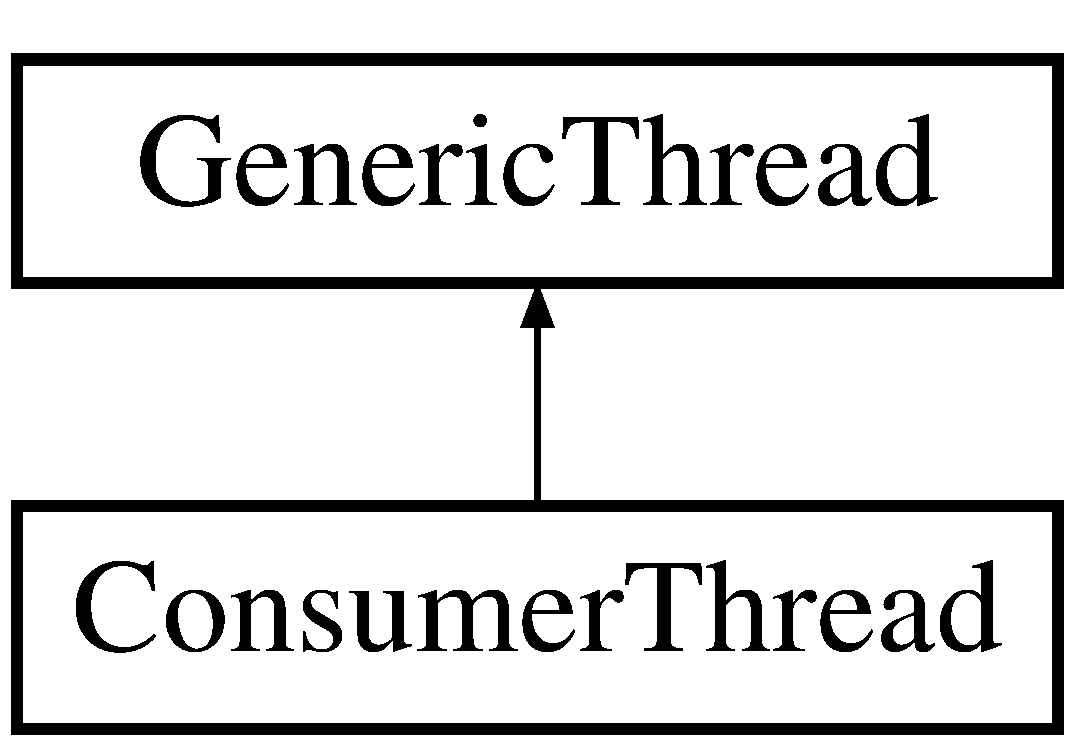
\includegraphics[height=2.000000cm]{classConsumerThread}
\end{center}
\end{figure}
\subsection*{Public Member Functions}
\begin{DoxyCompactItemize}
\item 
\hypertarget{classConsumerThread_a000214667d1ad9d31ce7133f6fbf9aac}{{\bfseries Consumer\-Thread} (\hyperlink{classGenericQueue}{Generic\-Queue}$<$ \hyperlink{classWorkItem}{Work\-Item} $\ast$ $>$ \&queue)}\label{classConsumerThread_a000214667d1ad9d31ce7133f6fbf9aac}

\item 
\hypertarget{classConsumerThread_a8fde7a9b6c2c0b3c62a9fd3c50296557}{void $\ast$ {\bfseries run} ()}\label{classConsumerThread_a8fde7a9b6c2c0b3c62a9fd3c50296557}

\end{DoxyCompactItemize}


The documentation for this class was generated from the following file\-:\begin{DoxyCompactItemize}
\item 
src/store/gqueue.\-cpp\end{DoxyCompactItemize}

\hypertarget{classEGOneStepGen}{}\section{E\+G\+One\+Step\+Gen Class Reference}
\label{classEGOneStepGen}\index{E\+G\+One\+Step\+Gen@{E\+G\+One\+Step\+Gen}}
Inheritance diagram for E\+G\+One\+Step\+Gen\+:\begin{figure}[H]
\begin{center}
\leavevmode
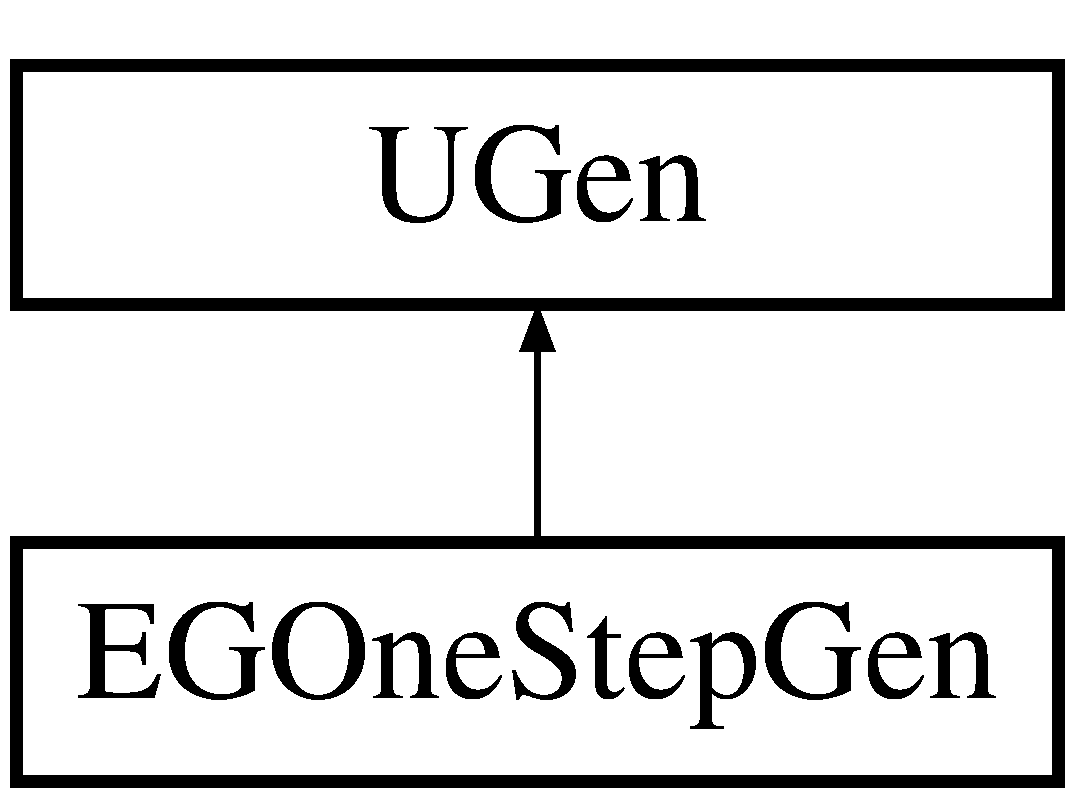
\includegraphics[height=2.000000cm]{classEGOneStepGen}
\end{center}
\end{figure}
\subsection*{Public Member Functions}
\begin{DoxyCompactItemize}
\item 
{\bfseries E\+G\+One\+Step\+Gen} (std\+::string name)\hypertarget{classEGOneStepGen_a9bc697acabed6c7b0467369ba073ede1}{}\label{classEGOneStepGen_a9bc697acabed6c7b0467369ba073ede1}

\item 
float {\bfseries tick} ()\hypertarget{classEGOneStepGen_a74df96649d7a66d19cb33bf9bf13f54a}{}\label{classEGOneStepGen_a74df96649d7a66d19cb33bf9bf13f54a}

\item 
void {\bfseries control} (std\+::string port\+Name, float value)\hypertarget{classEGOneStepGen_a8979594fb226c732a9b8232664f09047}{}\label{classEGOneStepGen_a8979594fb226c732a9b8232664f09047}

\item 
bool {\bfseries finished} ()\hypertarget{classEGOneStepGen_ae9f187e0f266559a80e4f4b534d79f78}{}\label{classEGOneStepGen_ae9f187e0f266559a80e4f4b534d79f78}

\item 
void {\bfseries set\+Duration} (float seconds)\hypertarget{classEGOneStepGen_aaf02138e168cad06cb955944f57ce93c}{}\label{classEGOneStepGen_aaf02138e168cad06cb955944f57ce93c}

\item 
void {\bfseries set\+Start\+Level} (float level)\hypertarget{classEGOneStepGen_af2b5bd8522fac9dc997d78d3750cdbbb}{}\label{classEGOneStepGen_af2b5bd8522fac9dc997d78d3750cdbbb}

\item 
void {\bfseries set\+End\+Level} (float level)\hypertarget{classEGOneStepGen_a3d58403aa5bebffeaf3f326855e0a233}{}\label{classEGOneStepGen_a3d58403aa5bebffeaf3f326855e0a233}

\item 
void {\bfseries reset} ()\hypertarget{classEGOneStepGen_a4898b08a0687e03802abdb7945708cab}{}\label{classEGOneStepGen_a4898b08a0687e03802abdb7945708cab}

\end{DoxyCompactItemize}
\subsection*{Additional Inherited Members}


The documentation for this class was generated from the following files\+:\begin{DoxyCompactItemize}
\item 
unit/E\+G\+One\+Step\+Gen.\+h\item 
unit/E\+G\+One\+Step\+Gen.\+cpp\end{DoxyCompactItemize}

\hypertarget{classEGUpDownGen}{}\section{E\+G\+Up\+Down\+Gen Class Reference}
\label{classEGUpDownGen}\index{E\+G\+Up\+Down\+Gen@{E\+G\+Up\+Down\+Gen}}
Inheritance diagram for E\+G\+Up\+Down\+Gen\+:\begin{figure}[H]
\begin{center}
\leavevmode
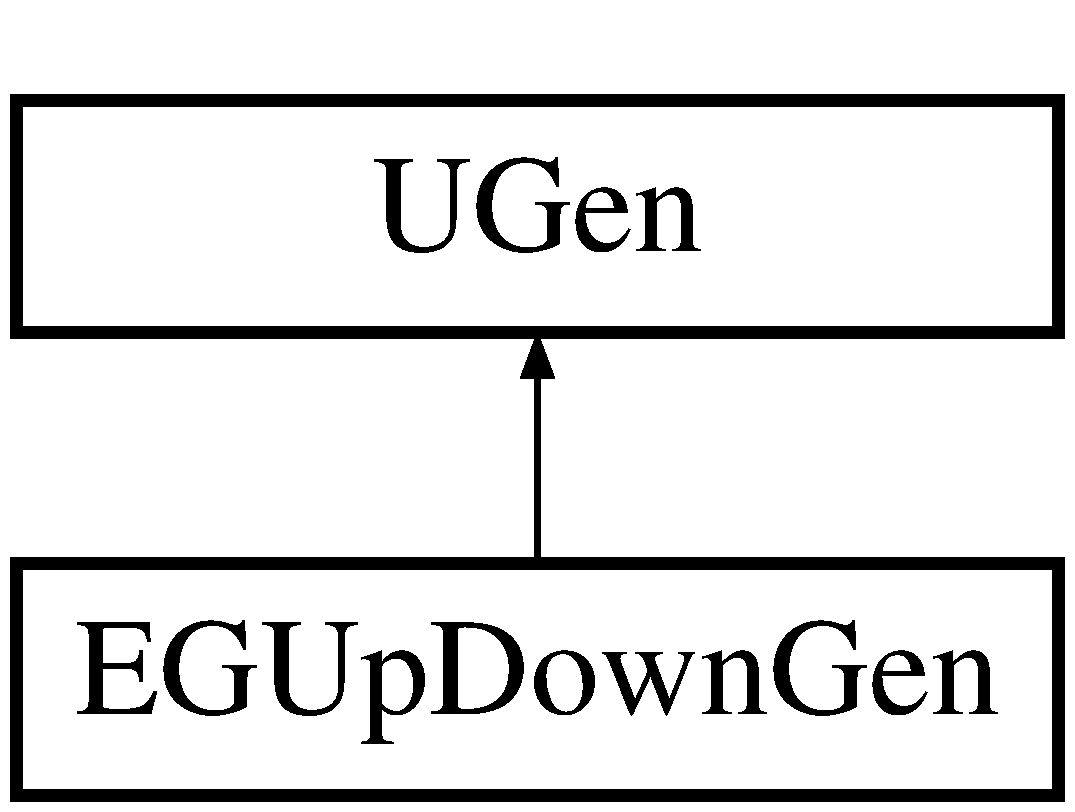
\includegraphics[height=2.000000cm]{classEGUpDownGen}
\end{center}
\end{figure}
\subsection*{Public Member Functions}
\begin{DoxyCompactItemize}
\item 
{\bfseries E\+G\+Up\+Down\+Gen} (std\+::string name)\hypertarget{classEGUpDownGen_abc35a572da36fa26f4b54beabfc6268e}{}\label{classEGUpDownGen_abc35a572da36fa26f4b54beabfc6268e}

\item 
float {\bfseries tick} ()\hypertarget{classEGUpDownGen_abea11de5389345064a8395d54411e3b3}{}\label{classEGUpDownGen_abea11de5389345064a8395d54411e3b3}

\item 
void {\bfseries control} (std\+::string port\+Name, float value)\hypertarget{classEGUpDownGen_ac1ef59d9023034c17b46e09bfae15178}{}\label{classEGUpDownGen_ac1ef59d9023034c17b46e09bfae15178}

\end{DoxyCompactItemize}
\subsection*{Additional Inherited Members}


The documentation for this class was generated from the following files\+:\begin{DoxyCompactItemize}
\item 
unit/E\+G\+Up\+Down\+Gen.\+h\item 
unit/E\+G\+Up\+Down\+Gen.\+cpp\end{DoxyCompactItemize}

\hypertarget{classExamplePacketListener}{}\section{Example\+Packet\+Listener Class Reference}
\label{classExamplePacketListener}\index{Example\+Packet\+Listener@{Example\+Packet\+Listener}}
Inheritance diagram for Example\+Packet\+Listener\+:\begin{figure}[H]
\begin{center}
\leavevmode
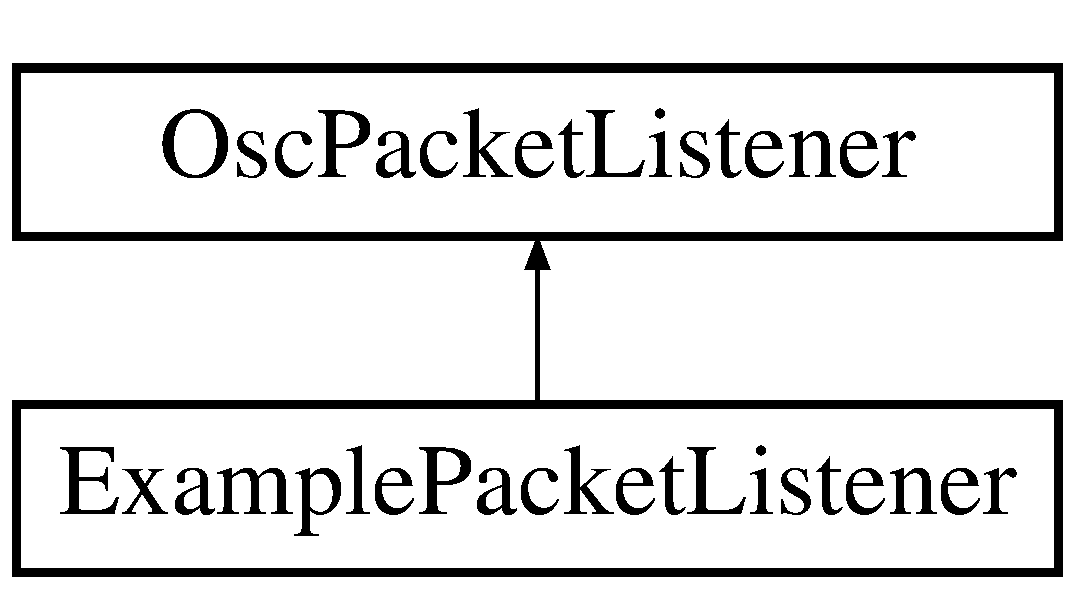
\includegraphics[height=2.000000cm]{classExamplePacketListener}
\end{center}
\end{figure}
\subsection*{Protected Member Functions}
\begin{DoxyCompactItemize}
\item 
virtual void {\bfseries Process\+Message} (const osc\+::\+Received\+Message \&m, const Ip\+Endpoint\+Name \&remote\+Endpoint)\hypertarget{classExamplePacketListener_a688ed2a3ec01d0fb7661f4fe0ffc90df}{}\label{classExamplePacketListener_a688ed2a3ec01d0fb7661f4fe0ffc90df}

\end{DoxyCompactItemize}


The documentation for this class was generated from the following file\+:\begin{DoxyCompactItemize}
\item 
Simple\+Receive.\+cpp\end{DoxyCompactItemize}

\hypertarget{classGatedConstantGen}{}\section{Gated\+Constant\+Gen Class Reference}
\label{classGatedConstantGen}\index{Gated\+Constant\+Gen@{Gated\+Constant\+Gen}}
Inheritance diagram for Gated\+Constant\+Gen\+:\begin{figure}[H]
\begin{center}
\leavevmode
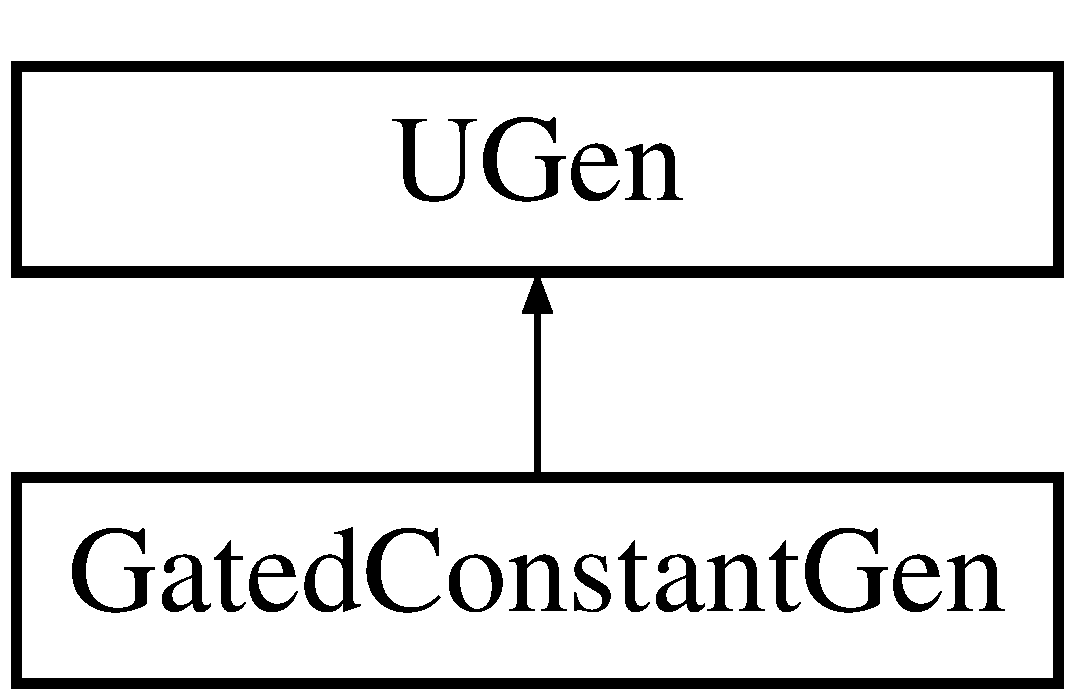
\includegraphics[height=2.000000cm]{classGatedConstantGen}
\end{center}
\end{figure}
\subsection*{Public Member Functions}
\begin{DoxyCompactItemize}
\item 
{\bfseries Gated\+Constant\+Gen} (std\+::string name)\hypertarget{classGatedConstantGen_ad30ad26411f421228c8f7075b4d27f9a}{}\label{classGatedConstantGen_ad30ad26411f421228c8f7075b4d27f9a}

\item 
void {\bfseries control} (std\+::string port\+Name, float value)\hypertarget{classGatedConstantGen_a8365ddc2a6ddebc86e196fa381a5648d}{}\label{classGatedConstantGen_a8365ddc2a6ddebc86e196fa381a5648d}

\item 
float {\bfseries tick} ()\hypertarget{classGatedConstantGen_aafff659359fed9f28c703acd0076c081}{}\label{classGatedConstantGen_aafff659359fed9f28c703acd0076c081}

\end{DoxyCompactItemize}
\subsection*{Additional Inherited Members}


The documentation for this class was generated from the following files\+:\begin{DoxyCompactItemize}
\item 
unit/Gated\+Constant\+Gen.\+h\item 
unit/Gated\+Constant\+Gen.\+cpp\end{DoxyCompactItemize}

\hypertarget{classGenericQueue}{\section{Generic\-Queue$<$ T $>$ Class Template Reference}
\label{classGenericQueue}\index{Generic\-Queue$<$ T $>$@{Generic\-Queue$<$ T $>$}}
}
\subsection*{Public Member Functions}
\begin{DoxyCompactItemize}
\item 
\hypertarget{classGenericQueue_af5de20e93f3ee8d1fdd38a8ec1ae52f6}{void {\bfseries add} (T item)}\label{classGenericQueue_af5de20e93f3ee8d1fdd38a8ec1ae52f6}

\item 
\hypertarget{classGenericQueue_a15366cdc3234d238c664c82524f14c0b}{T {\bfseries remove} ()}\label{classGenericQueue_a15366cdc3234d238c664c82524f14c0b}

\item 
\hypertarget{classGenericQueue_aa94c712ca621ef5c121cd4f9c9188f67}{int {\bfseries size} ()}\label{classGenericQueue_aa94c712ca621ef5c121cd4f9c9188f67}

\item 
\hypertarget{classGenericQueue_a0fd02ceeecaf5c0903e3ee7199b183bc}{void {\bfseries clear} ()}\label{classGenericQueue_a0fd02ceeecaf5c0903e3ee7199b183bc}

\end{DoxyCompactItemize}


The documentation for this class was generated from the following file\-:\begin{DoxyCompactItemize}
\item 
src/include/Generic\-Queue.\-h\end{DoxyCompactItemize}

\hypertarget{classGenericThread}{}\section{Generic\+Thread Class Reference}
\label{classGenericThread}\index{Generic\+Thread@{Generic\+Thread}}
Inheritance diagram for Generic\+Thread\+:\begin{figure}[H]
\begin{center}
\leavevmode
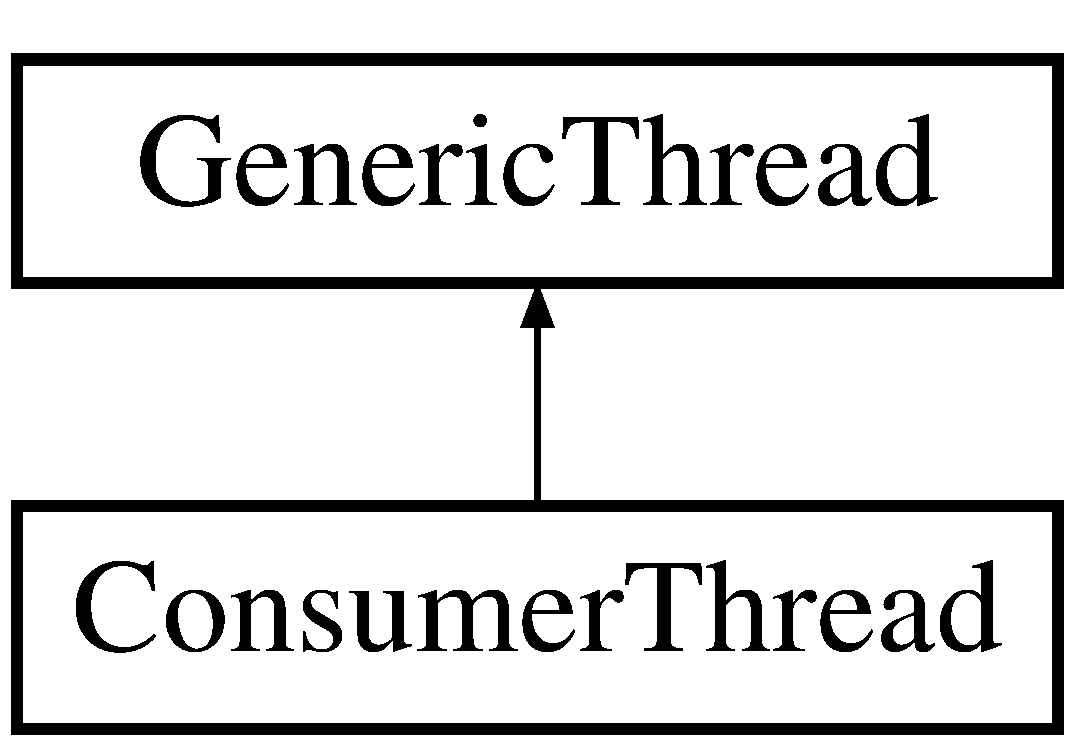
\includegraphics[height=2.000000cm]{classGenericThread}
\end{center}
\end{figure}
\subsection*{Public Member Functions}
\begin{DoxyCompactItemize}
\item 
int {\bfseries start} ()\hypertarget{classGenericThread_ac1d8c3d7dcaae01e89c69093a065141f}{}\label{classGenericThread_ac1d8c3d7dcaae01e89c69093a065141f}

\item 
int {\bfseries join} ()\hypertarget{classGenericThread_a217ef41077ae00ce48372c03838af96a}{}\label{classGenericThread_a217ef41077ae00ce48372c03838af96a}

\item 
int {\bfseries detach} ()\hypertarget{classGenericThread_abd0849015ec4004b789aa3181853fbf6}{}\label{classGenericThread_abd0849015ec4004b789aa3181853fbf6}

\item 
pthread\+\_\+t {\bfseries self} ()\hypertarget{classGenericThread_a0ac1c8aa0c6f5d47d73626c13854d444}{}\label{classGenericThread_a0ac1c8aa0c6f5d47d73626c13854d444}

\item 
virtual void $\ast$ {\bfseries run} ()=0\hypertarget{classGenericThread_a54147ff9f16e7985e634b5f0d6d5b7f9}{}\label{classGenericThread_a54147ff9f16e7985e634b5f0d6d5b7f9}

\end{DoxyCompactItemize}


The documentation for this class was generated from the following files\+:\begin{DoxyCompactItemize}
\item 
store/Generic\+Thread.\+h\item 
store/Generic\+Thread.\+cpp\end{DoxyCompactItemize}

\hypertarget{classIDGenerator}{\section{I\-D\-Generator Class Reference}
\label{classIDGenerator}\index{I\-D\-Generator@{I\-D\-Generator}}
}
\subsection*{Public Member Functions}
\begin{DoxyCompactItemize}
\item 
\hypertarget{classIDGenerator_a223bf057a0ad9e69df527142dfe1e91b}{std\-::string {\bfseries next\-I\-D} ()}\label{classIDGenerator_a223bf057a0ad9e69df527142dfe1e91b}

\end{DoxyCompactItemize}


The documentation for this class was generated from the following files\-:\begin{DoxyCompactItemize}
\item 
include/I\-D\-Generator.\-h\item 
util/I\-D\-Generator.\-cpp\end{DoxyCompactItemize}

\hypertarget{classInterpolation}{}\section{Interpolation Class Reference}
\label{classInterpolation}\index{Interpolation@{Interpolation}}


{\ttfamily \#include $<$Interpolation.\+h$>$}

\subsection*{Static Public Member Functions}
\begin{DoxyCompactItemize}
\item 
static float {\bfseries map} (float value, float s1, float e1, float s2, float e2)\hypertarget{classInterpolation_adfd3003c39c40ec76342274c65017761}{}\label{classInterpolation_adfd3003c39c40ec76342274c65017761}

\item 
static float {\bfseries map} (int value, int s1, int e1, float s2, float e2)\hypertarget{classInterpolation_ac6eab12deb9f79b79200aad3b219e7c3}{}\label{classInterpolation_ac6eab12deb9f79b79200aad3b219e7c3}

\item 
static int {\bfseries discrete} (float value, float s1, float e1, int max)\hypertarget{classInterpolation_a246c72a835822b7674758d657ed44230}{}\label{classInterpolation_a246c72a835822b7674758d657ed44230}

\item 
static float \hyperlink{classInterpolation_a5549f8859f14153da891222a8ff1a22f}{maplog} (float value, float s1, float e1, float s2, float e2)
\item 
static float {\bfseries mapexp} (float value, float s1, float e1, float s2, float e2)\hypertarget{classInterpolation_a08d1fe5e82708ab26a019e9ae9f851c8}{}\label{classInterpolation_a08d1fe5e82708ab26a019e9ae9f851c8}

\end{DoxyCompactItemize}


\subsection{Detailed Description}
\hyperlink{classInterpolation}{Interpolation} provides a number of helper function to easily calculate the linear interpolation of a value.

\begin{DoxyAuthor}{Author}
jtm 
\end{DoxyAuthor}
\begin{DoxySince}{Since}
04-\/2016 
\end{DoxySince}
\begin{DoxyVersion}{Version}
1.\+0 
\end{DoxyVersion}


\subsection{Member Function Documentation}
\index{Interpolation@{Interpolation}!maplog@{maplog}}
\index{maplog@{maplog}!Interpolation@{Interpolation}}
\subsubsection[{\texorpdfstring{maplog(float value, float s1, float e1, float s2, float e2)}{maplog(float value, float s1, float e1, float s2, float e2)}}]{\setlength{\rightskip}{0pt plus 5cm}float Interpolation\+::maplog (
\begin{DoxyParamCaption}
\item[{float}]{value, }
\item[{float}]{s1, }
\item[{float}]{e1, }
\item[{float}]{s2, }
\item[{float}]{e2}
\end{DoxyParamCaption}
)\hspace{0.3cm}{\ttfamily [static]}}\hypertarget{classInterpolation_a5549f8859f14153da891222a8ff1a22f}{}\label{classInterpolation_a5549f8859f14153da891222a8ff1a22f}
Calculates the logarithm() of the linear mapping of the input value from interval \mbox{[}s1,e1\mbox{]} to interval \mbox{[}s2,e2\mbox{]}.


\begin{DoxyItemize}
\item The logarithmic result allows for a more fine grained control of the {\bfseries higher} end of the interval.
\item The result should be normalized by dividing the result by log(e2-\/s2).
\end{DoxyItemize}

\begin{DoxyReturn}{Returns}
The log() of the linear mapping.
\end{DoxyReturn}

\begin{DoxyParams}{Parameters}
{\em value} & the value to be mapped (e.\+g. a knob value) \\
\hline
{\em s1} & start of domain interval \\
\hline
{\em e1} & end of domain interval \\
\hline
{\em s2} & start of range interval \\
\hline
{\em e2} & end of range interval \\
\hline
\end{DoxyParams}


The documentation for this class was generated from the following files\+:\begin{DoxyCompactItemize}
\item 
include/Interpolation.\+h\item 
util/Interpolation.\+cpp\end{DoxyCompactItemize}

\hypertarget{classMessageData}{}\section{Message\+Data Class Reference}
\label{classMessageData}\index{Message\+Data@{Message\+Data}}
\subsection*{Public Types}
\begin{DoxyCompactItemize}
\item 
enum {\bfseries Types} \{ \\*
{\bfseries M\+I\+D\+I\+ON}, 
{\bfseries M\+I\+D\+I\+O\+FF}, 
{\bfseries C\+O\+N\+T\+R\+OL}, 
{\bfseries P\+A\+D\+ON}, 
\\*
{\bfseries P\+A\+D\+O\+FF}, 
{\bfseries S\+L\+I\+D\+ER}, 
{\bfseries U\+N\+K\+N\+O\+WN}
 \}\hypertarget{classMessageData_a63f99930873414c0908b5e735964e022}{}\label{classMessageData_a63f99930873414c0908b5e735964e022}

\end{DoxyCompactItemize}
\subsection*{Public Member Functions}
\begin{DoxyCompactItemize}
\item 
{\bfseries Message\+Data} (std\+::string s, int a1, int a2, int a3, float f)\hypertarget{classMessageData_af370333b9828ad63ba1031ac941300c2}{}\label{classMessageData_af370333b9828ad63ba1031ac941300c2}

\item 
{\bfseries Message\+Data} (\hyperlink{classMessageData}{Message\+Data} $\ast$md)\hypertarget{classMessageData_acf5694351e2f877340d6b38044d8b2d3}{}\label{classMessageData_acf5694351e2f877340d6b38044d8b2d3}

\item 
std\+::string {\bfseries get\+Message} ()\hypertarget{classMessageData_a8bf658a5be5789142fa260512fded9a1}{}\label{classMessageData_a8bf658a5be5789142fa260512fded9a1}

\item 
int {\bfseries get\+Code} ()\hypertarget{classMessageData_aa625a45bf78b8351d29a7696c8f014e9}{}\label{classMessageData_aa625a45bf78b8351d29a7696c8f014e9}

\item 
int {\bfseries get\+Key} ()\hypertarget{classMessageData_ab70773361a5ffba488a83b0d87cfb25c}{}\label{classMessageData_ab70773361a5ffba488a83b0d87cfb25c}

\item 
int {\bfseries get\+Value} ()\hypertarget{classMessageData_af79bf248fbb542bd25984f7f2b3993eb}{}\label{classMessageData_af79bf248fbb542bd25984f7f2b3993eb}

\item 
float {\bfseries get\+F1} ()\hypertarget{classMessageData_ad1e951e980e59c5d222b79856cae6d32}{}\label{classMessageData_ad1e951e980e59c5d222b79856cae6d32}

\item 
Types {\bfseries get\+Type} ()\hypertarget{classMessageData_a38c69b7ebcf46e7c19ff2409af36a7ae}{}\label{classMessageData_a38c69b7ebcf46e7c19ff2409af36a7ae}

\item 
void {\bfseries set\+Message} (std\+::string s)\hypertarget{classMessageData_a1da8f45a1453c7d11029fa360d7a642c}{}\label{classMessageData_a1da8f45a1453c7d11029fa360d7a642c}

\item 
void {\bfseries adapt\+Message\+Type} ()\hypertarget{classMessageData_a0f8ce5f6d5c4452e26656236ee7aefc3}{}\label{classMessageData_a0f8ce5f6d5c4452e26656236ee7aefc3}

\item 
void {\bfseries set\+Code} (int a1)\hypertarget{classMessageData_a8639583a844208ccae9568bb68d1e547}{}\label{classMessageData_a8639583a844208ccae9568bb68d1e547}

\item 
void {\bfseries set\+Key} (int a2)\hypertarget{classMessageData_a54a0ddfb44fba671ba243914b037e231}{}\label{classMessageData_a54a0ddfb44fba671ba243914b037e231}

\item 
void {\bfseries set\+Value} (int a3)\hypertarget{classMessageData_a24e273f0a4443505ccf6222405cfb567}{}\label{classMessageData_a24e273f0a4443505ccf6222405cfb567}

\item 
void {\bfseries set\+F1} (float f)\hypertarget{classMessageData_a94dce06ace95a93c075dbaf253e559fe}{}\label{classMessageData_a94dce06ace95a93c075dbaf253e559fe}

\item 
void {\bfseries set\+Message\+Data} (std\+::string s, int a1, int a2, int a3, float f)\hypertarget{classMessageData_a9eb7741e4216075b0e03c554d83e35ae}{}\label{classMessageData_a9eb7741e4216075b0e03c554d83e35ae}

\item 
bool {\bfseries is\+Fresh} ()\hypertarget{classMessageData_a169f4e7ec5a0eb896cfccd8186b5fe8d}{}\label{classMessageData_a169f4e7ec5a0eb896cfccd8186b5fe8d}

\end{DoxyCompactItemize}


The documentation for this class was generated from the following files\+:\begin{DoxyCompactItemize}
\item 
osc/Message\+Data.\+h\item 
osc/Message\+Data.\+cpp\end{DoxyCompactItemize}

\hypertarget{classMessageDataQueue}{}\section{Message\+Data\+Queue Class Reference}
\label{classMessageDataQueue}\index{Message\+Data\+Queue@{Message\+Data\+Queue}}
\subsection*{Public Member Functions}
\begin{DoxyCompactItemize}
\item 
void {\bfseries add} (\hyperlink{classMessageData}{Message\+Data} $\ast$m)\hypertarget{classMessageDataQueue_aa31f6a8bed7000525d09716de264a049}{}\label{classMessageDataQueue_aa31f6a8bed7000525d09716de264a049}

\item 
\hyperlink{classMessageData}{Message\+Data} $\ast$ {\bfseries get} ()\hypertarget{classMessageDataQueue_ace0bab37a7339c7a0eb813f80a03c88d}{}\label{classMessageDataQueue_ace0bab37a7339c7a0eb813f80a03c88d}

\item 
int {\bfseries size} ()\hypertarget{classMessageDataQueue_a6f7619c03371e76b95a2c2d348da866d}{}\label{classMessageDataQueue_a6f7619c03371e76b95a2c2d348da866d}

\item 
void {\bfseries clear} ()\hypertarget{classMessageDataQueue_a565232895a0e0cc0416715aedf2e5e21}{}\label{classMessageDataQueue_a565232895a0e0cc0416715aedf2e5e21}

\end{DoxyCompactItemize}


The documentation for this class was generated from the following files\+:\begin{DoxyCompactItemize}
\item 
store/Message\+Data\+Queue.\+h\item 
store/Message\+Data\+Queue.\+cpp\end{DoxyCompactItemize}

\hypertarget{classMidiConnector}{}\section{Midi\+Connector Class Reference}
\label{classMidiConnector}\index{Midi\+Connector@{Midi\+Connector}}
\subsection*{Public Member Functions}
\begin{DoxyCompactItemize}
\item 
{\bfseries Midi\+Connector} (int p)\hypertarget{classMidiConnector_a1629e8c842409a21dbc78258794556cc}{}\label{classMidiConnector_a1629e8c842409a21dbc78258794556cc}

\item 
void {\bfseries send\+Message} (std\+::string message\+Type, int code, int key, int value, float f1)\hypertarget{classMidiConnector_a700ee4383b29cd2bdc73f7cfc61a360e}{}\label{classMidiConnector_a700ee4383b29cd2bdc73f7cfc61a360e}

\end{DoxyCompactItemize}


The documentation for this class was generated from the following files\+:\begin{DoxyCompactItemize}
\item 
osc/Midi\+Connector.\+h\item 
osc/Midi\+Connector.\+cpp\end{DoxyCompactItemize}

\hypertarget{classOscInConnector_1_1MidiPacketListener}{}\section{Osc\+In\+Connector\+:\+:Midi\+Packet\+Listener Class Reference}
\label{classOscInConnector_1_1MidiPacketListener}\index{Osc\+In\+Connector\+::\+Midi\+Packet\+Listener@{Osc\+In\+Connector\+::\+Midi\+Packet\+Listener}}
Inheritance diagram for Osc\+In\+Connector\+:\+:Midi\+Packet\+Listener\+:\begin{figure}[H]
\begin{center}
\leavevmode
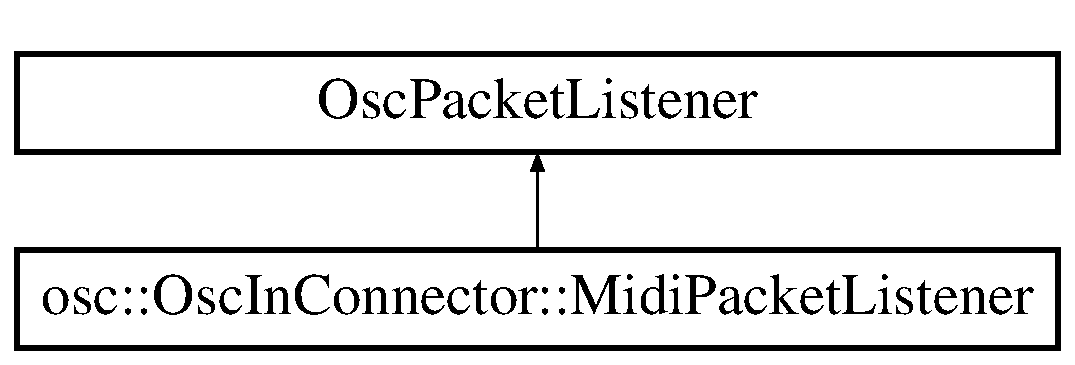
\includegraphics[height=2.000000cm]{classOscInConnector_1_1MidiPacketListener}
\end{center}
\end{figure}
\subsection*{Public Member Functions}
\begin{DoxyCompactItemize}
\item 
void {\bfseries set\+Osc\+In} (\hyperlink{classOscInConnector}{Osc\+In\+Connector} $\ast$o)\hypertarget{classOscInConnector_1_1MidiPacketListener_ab4e0346cad409b3871add20bc5c8c904}{}\label{classOscInConnector_1_1MidiPacketListener_ab4e0346cad409b3871add20bc5c8c904}

\item 
int {\bfseries get\+Port} ()\hypertarget{classOscInConnector_1_1MidiPacketListener_affd65358cd1ffcde113576b8023fa8d6}{}\label{classOscInConnector_1_1MidiPacketListener_affd65358cd1ffcde113576b8023fa8d6}

\end{DoxyCompactItemize}
\subsection*{Protected Member Functions}
\begin{DoxyCompactItemize}
\item 
void {\bfseries write\+Data} (std\+::string s, int a1, int a2, int a3, float f)\hypertarget{classOscInConnector_1_1MidiPacketListener_a6ad19bb71d7d360d432eecd4d2f8aa0f}{}\label{classOscInConnector_1_1MidiPacketListener_a6ad19bb71d7d360d432eecd4d2f8aa0f}

\item 
virtual void {\bfseries Process\+Message} (const osc\+::\+Received\+Message \&m, const Ip\+Endpoint\+Name \&remote\+Endpoint)\hypertarget{classOscInConnector_1_1MidiPacketListener_ad5b4e469c87859e8577d2bf77aaa66bd}{}\label{classOscInConnector_1_1MidiPacketListener_ad5b4e469c87859e8577d2bf77aaa66bd}

\end{DoxyCompactItemize}


The documentation for this class was generated from the following file\+:\begin{DoxyCompactItemize}
\item 
Osc\+In\+Connector.\+cpp\end{DoxyCompactItemize}

\hypertarget{classMultiplyGen}{}\section{Multiply\+Gen Class Reference}
\label{classMultiplyGen}\index{Multiply\+Gen@{Multiply\+Gen}}
Inheritance diagram for Multiply\+Gen\+:\begin{figure}[H]
\begin{center}
\leavevmode
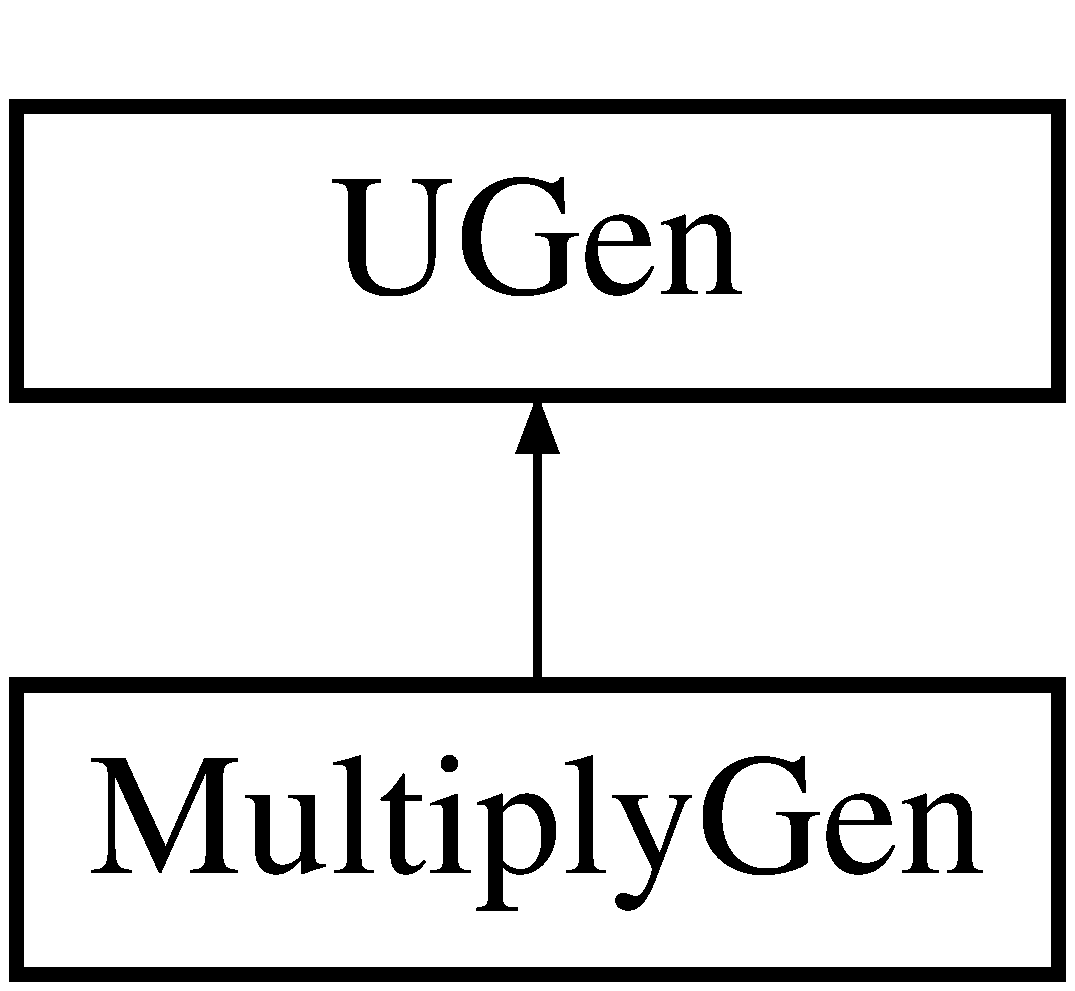
\includegraphics[height=2.000000cm]{classMultiplyGen}
\end{center}
\end{figure}
\subsection*{Public Member Functions}
\begin{DoxyCompactItemize}
\item 
{\bfseries Multiply\+Gen} (std\+::string name)\hypertarget{classMultiplyGen_a8c63aba9e9be634e03f900182b4a1d7a}{}\label{classMultiplyGen_a8c63aba9e9be634e03f900182b4a1d7a}

\item 
void {\bfseries control} (std\+::string port\+Name, float value)\hypertarget{classMultiplyGen_a399981309ef24f24c7044172e58c1e8a}{}\label{classMultiplyGen_a399981309ef24f24c7044172e58c1e8a}

\item 
float {\bfseries tick} ()\hypertarget{classMultiplyGen_abeeb8a84f91375454120639a9bb810fb}{}\label{classMultiplyGen_abeeb8a84f91375454120639a9bb810fb}

\end{DoxyCompactItemize}
\subsection*{Additional Inherited Members}


The documentation for this class was generated from the following files\+:\begin{DoxyCompactItemize}
\item 
unit/Multiply\+Gen.\+h\item 
unit/Multiply\+Gen.\+cpp\end{DoxyCompactItemize}

\hypertarget{classMultiplyTwoGen}{}\section{Multiply\+Two\+Gen Class Reference}
\label{classMultiplyTwoGen}\index{Multiply\+Two\+Gen@{Multiply\+Two\+Gen}}
Inheritance diagram for Multiply\+Two\+Gen\+:\begin{figure}[H]
\begin{center}
\leavevmode
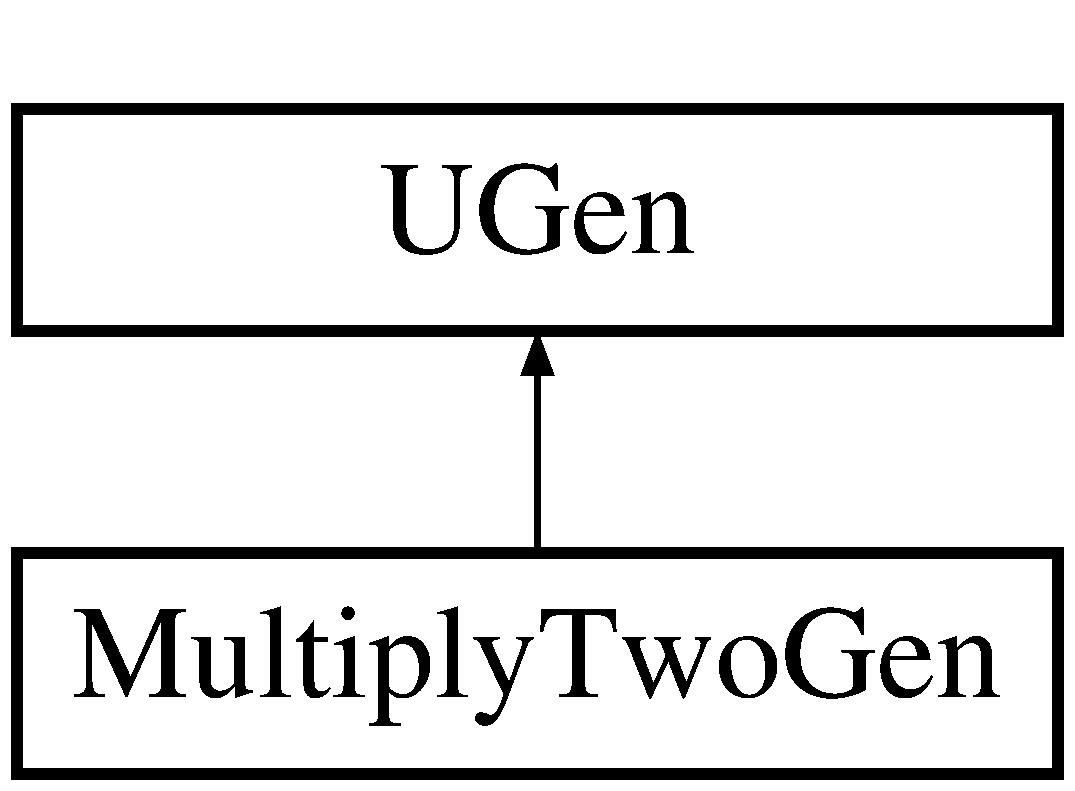
\includegraphics[height=2.000000cm]{classMultiplyTwoGen}
\end{center}
\end{figure}
\subsection*{Public Member Functions}
\begin{DoxyCompactItemize}
\item 
{\bfseries Multiply\+Two\+Gen} (std\+::string name)\hypertarget{classMultiplyTwoGen_a35e526170e8ac7a43fc19c2a78e14b44}{}\label{classMultiplyTwoGen_a35e526170e8ac7a43fc19c2a78e14b44}

\item 
void {\bfseries control} (std\+::string port\+Name, float value)\hypertarget{classMultiplyTwoGen_af8558651a63c73f27221e99ad03f3242}{}\label{classMultiplyTwoGen_af8558651a63c73f27221e99ad03f3242}

\item 
float {\bfseries tick} ()\hypertarget{classMultiplyTwoGen_a70a07ad9e0f67e6a50aadcdf902db8f3}{}\label{classMultiplyTwoGen_a70a07ad9e0f67e6a50aadcdf902db8f3}

\end{DoxyCompactItemize}
\subsection*{Additional Inherited Members}


The documentation for this class was generated from the following files\+:\begin{DoxyCompactItemize}
\item 
unit/Multiply\+Two\+Gen.\+h\item 
unit/Multiply\+Two\+Gen.\+cpp\end{DoxyCompactItemize}

\hypertarget{classNeonlicht}{}\section{Neonlicht Class Reference}
\label{classNeonlicht}\index{Neonlicht@{Neonlicht}}
\subsection*{Public Member Functions}
\begin{DoxyCompactItemize}
\item 
void {\bfseries configure} ()\hypertarget{classNeonlicht_a32ec4c221148d01bbafd1637ced9b130}{}\label{classNeonlicht_a32ec4c221148d01bbafd1637ced9b130}

\item 
void {\bfseries start} ()\hypertarget{classNeonlicht_aae54e46be4d251ce4e062cd777994a69}{}\label{classNeonlicht_aae54e46be4d251ce4e062cd777994a69}

\item 
void {\bfseries stop} ()\hypertarget{classNeonlicht_a9d1f643b1a2394f9cd181149f7558c72}{}\label{classNeonlicht_a9d1f643b1a2394f9cd181149f7558c72}

\item 
long {\bfseries get\+Stream\+Latency} ()\hypertarget{classNeonlicht_a4354cc2fa6d7bd22e89d1314e375f54f}{}\label{classNeonlicht_a4354cc2fa6d7bd22e89d1314e375f54f}

\end{DoxyCompactItemize}
\subsection*{Static Public Member Functions}
\begin{DoxyCompactItemize}
\item 
static int {\bfseries tick} (void $\ast$output\+Buffer, void $\ast$input\+Buffer, unsigned int n\+Buffer\+Frames, double stream\+Time, Rt\+Audio\+Stream\+Status status, void $\ast$data\+Pointer)\hypertarget{classNeonlicht_a57c3e8d4154418c9efc4b48d45b732d6}{}\label{classNeonlicht_a57c3e8d4154418c9efc4b48d45b732d6}

\end{DoxyCompactItemize}
\subsection*{Static Public Attributes}
\begin{DoxyCompactItemize}
\item 
static \hyperlink{classCentralStore}{Central\+Store} {\bfseries CS}\hypertarget{classNeonlicht_a1ac3a31190125df3763a9f3d2f085d5e}{}\label{classNeonlicht_a1ac3a31190125df3763a9f3d2f085d5e}

\item 
static int {\bfseries C\+NT} = 0\hypertarget{classNeonlicht_ac86fbdabd4683feaac58b4aefbdf6695}{}\label{classNeonlicht_ac86fbdabd4683feaac58b4aefbdf6695}

\end{DoxyCompactItemize}


The documentation for this class was generated from the following files\+:\begin{DoxyCompactItemize}
\item 
include/Neonlicht.\+h\item 
Neonlicht.\+cpp\end{DoxyCompactItemize}

\hypertarget{classNoiseGen}{}\section{Noise\+Gen Class Reference}
\label{classNoiseGen}\index{Noise\+Gen@{Noise\+Gen}}
Inheritance diagram for Noise\+Gen\+:\begin{figure}[H]
\begin{center}
\leavevmode
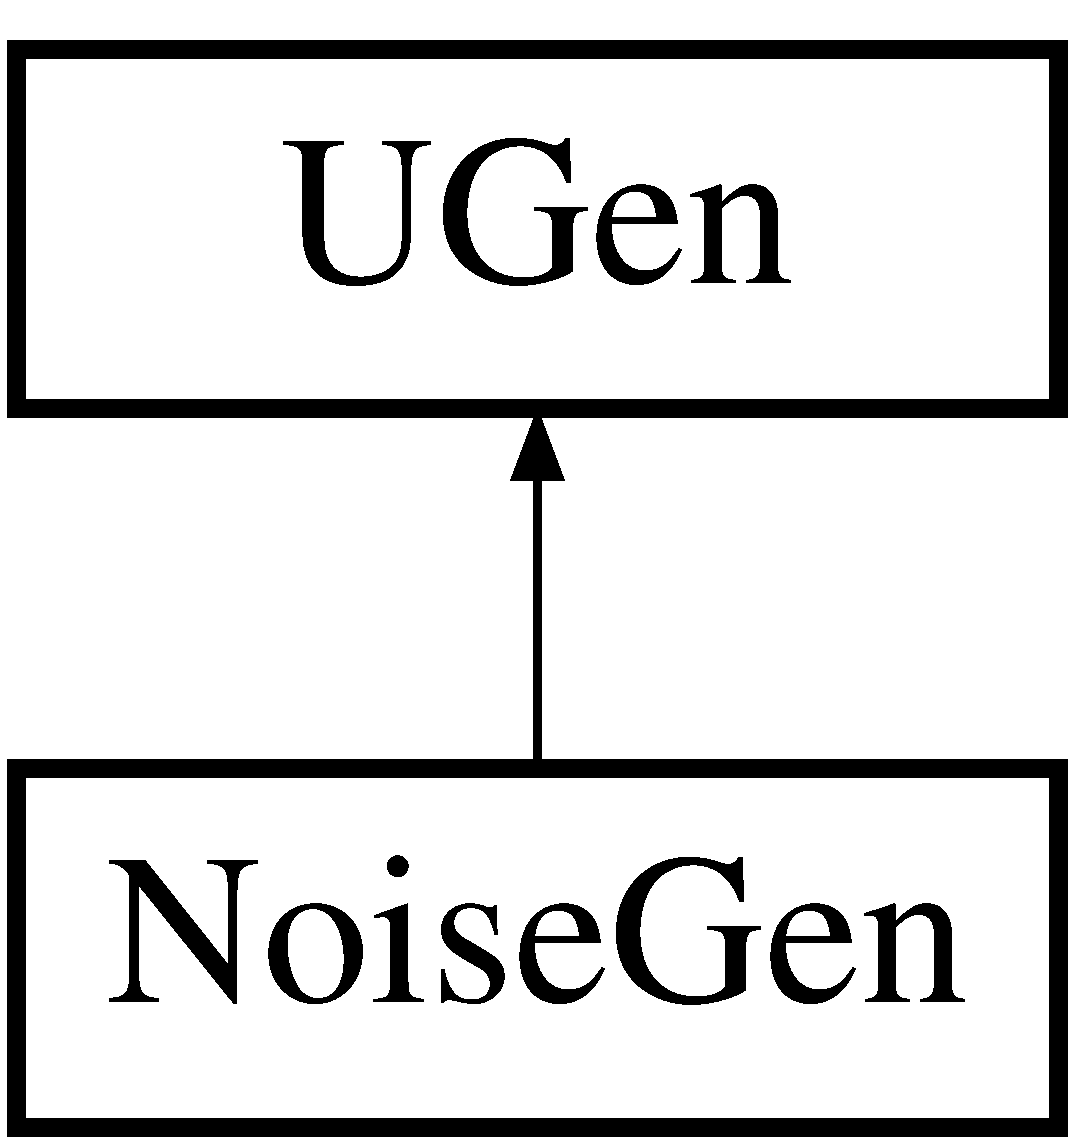
\includegraphics[height=2.000000cm]{classNoiseGen}
\end{center}
\end{figure}
\subsection*{Public Member Functions}
\begin{DoxyCompactItemize}
\item 
{\bfseries Noise\+Gen} (std\+::string name)\hypertarget{classNoiseGen_aa49d8817fff2757abc19f0dffea0c7fe}{}\label{classNoiseGen_aa49d8817fff2757abc19f0dffea0c7fe}

\item 
void {\bfseries control} (std\+::string port\+Name, float value)\hypertarget{classNoiseGen_a73628ae13d893658b88bc30eb43437ba}{}\label{classNoiseGen_a73628ae13d893658b88bc30eb43437ba}

\item 
float {\bfseries tick} ()\hypertarget{classNoiseGen_addaecf96df1cf9f1ba4875fb849949df}{}\label{classNoiseGen_addaecf96df1cf9f1ba4875fb849949df}

\end{DoxyCompactItemize}
\subsection*{Public Attributes}
\begin{DoxyCompactItemize}
\item 
long {\bfseries count} = 0\hypertarget{classNoiseGen_ae4bcbe827651898095ca99644663a05e}{}\label{classNoiseGen_ae4bcbe827651898095ca99644663a05e}

\end{DoxyCompactItemize}
\subsection*{Additional Inherited Members}


The documentation for this class was generated from the following files\+:\begin{DoxyCompactItemize}
\item 
unit/Noise\+Gen.\+h\item 
unit/Noise\+Gen.\+cpp\end{DoxyCompactItemize}

\hypertarget{classNoiseUnit}{}\section{Noise\+Unit Class Reference}
\label{classNoiseUnit}\index{Noise\+Unit@{Noise\+Unit}}
Inheritance diagram for Noise\+Unit\+:\begin{figure}[H]
\begin{center}
\leavevmode
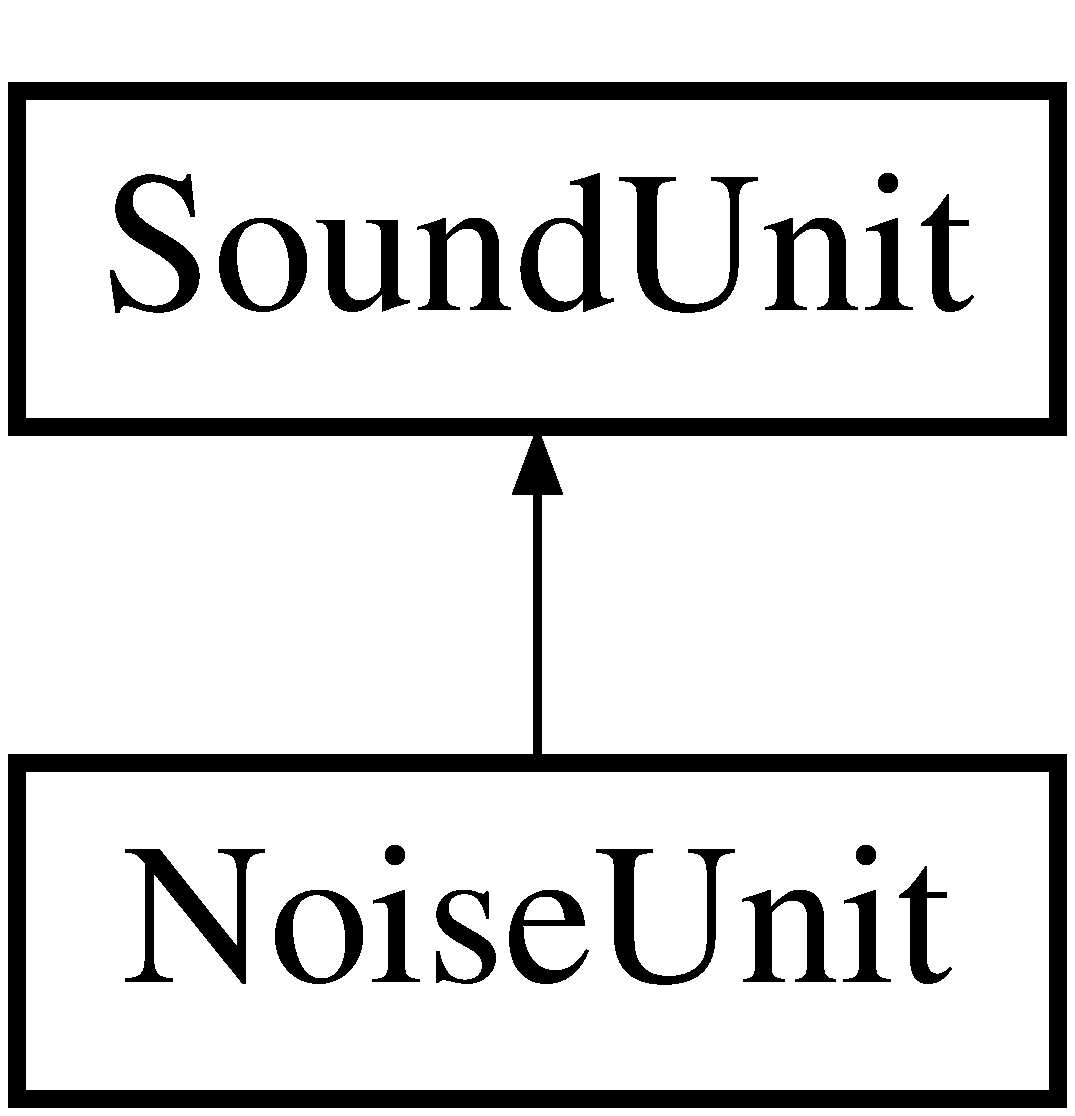
\includegraphics[height=2.000000cm]{classNoiseUnit}
\end{center}
\end{figure}
\subsection*{Public Member Functions}
\begin{DoxyCompactItemize}
\item 
void {\bfseries setup} ()\hypertarget{classNoiseUnit_a81666e8bdea833fad6a4451a765c6b83}{}\label{classNoiseUnit_a81666e8bdea833fad6a4451a765c6b83}

\item 
void {\bfseries control} (std\+::string port\+Name, float value)\hypertarget{classNoiseUnit_a7014ea85fb499bbe69fcf7ce96be8d32}{}\label{classNoiseUnit_a7014ea85fb499bbe69fcf7ce96be8d32}

\item 
float {\bfseries tick} ()\hypertarget{classNoiseUnit_af48a9a915f7f593105e8fe2d2ddb745a}{}\label{classNoiseUnit_af48a9a915f7f593105e8fe2d2ddb745a}

\end{DoxyCompactItemize}
\subsection*{Additional Inherited Members}


The documentation for this class was generated from the following files\+:\begin{DoxyCompactItemize}
\item 
unit/Noise\+Unit.\+h\item 
unit/Noise\+Unit.\+cpp\end{DoxyCompactItemize}

\hypertarget{classNumberGen}{}\section{Number\+Gen Class Reference}
\label{classNumberGen}\index{Number\+Gen@{Number\+Gen}}
Inheritance diagram for Number\+Gen\+:\begin{figure}[H]
\begin{center}
\leavevmode
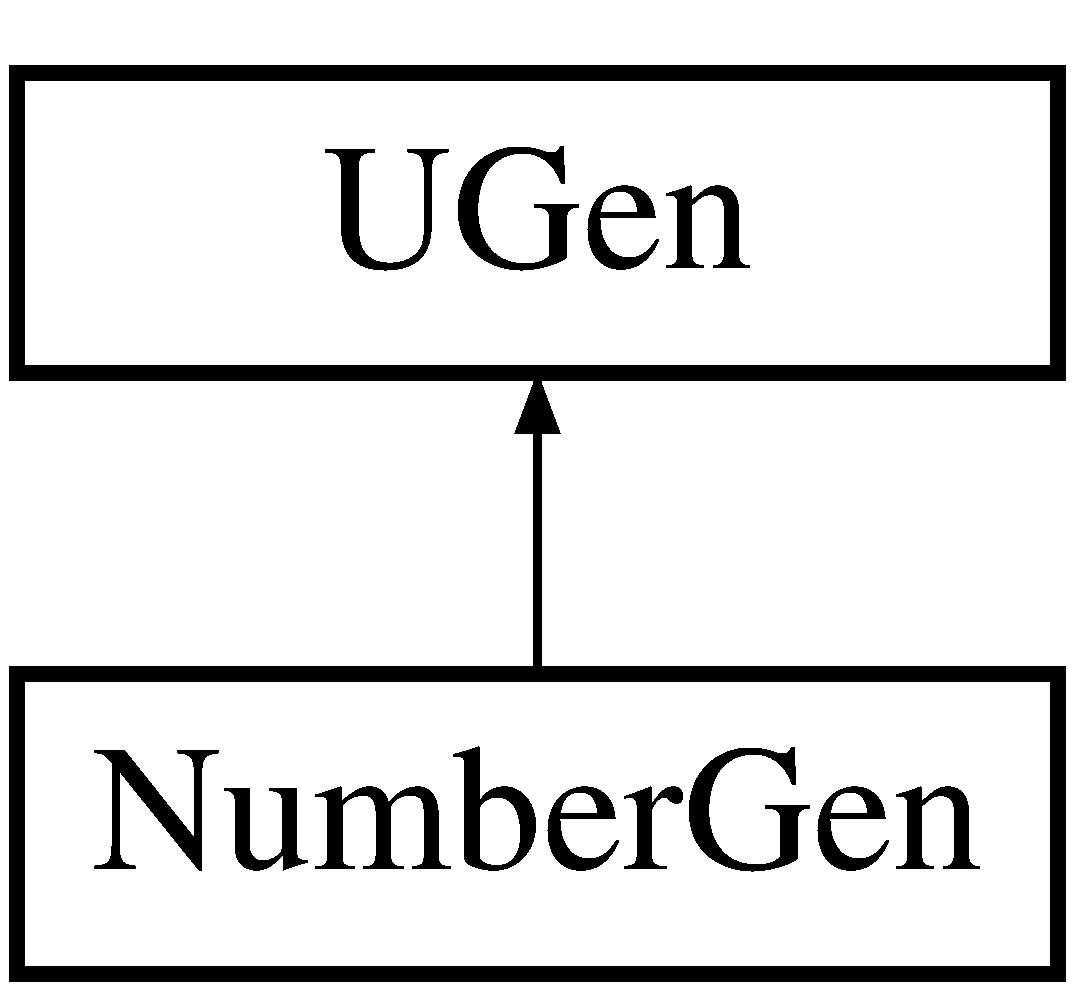
\includegraphics[height=2.000000cm]{classNumberGen}
\end{center}
\end{figure}
\subsection*{Public Member Functions}
\begin{DoxyCompactItemize}
\item 
{\bfseries Number\+Gen} (std\+::string name)\hypertarget{classNumberGen_a6e93812c4805a43f19f8fb11680e32a4}{}\label{classNumberGen_a6e93812c4805a43f19f8fb11680e32a4}

\item 
void {\bfseries control} (std\+::string port\+Name, float value)\hypertarget{classNumberGen_a9daaaf8a12389873494bb1ad2f877c8c}{}\label{classNumberGen_a9daaaf8a12389873494bb1ad2f877c8c}

\item 
float {\bfseries tick} ()\hypertarget{classNumberGen_a38cef7d64a12e40bf2ae14f29def41ca}{}\label{classNumberGen_a38cef7d64a12e40bf2ae14f29def41ca}

\end{DoxyCompactItemize}
\subsection*{Additional Inherited Members}


The documentation for this class was generated from the following files\+:\begin{DoxyCompactItemize}
\item 
unit/Number\+Gen.\+h\item 
unit/Number\+Gen.\+cpp\end{DoxyCompactItemize}

\hypertarget{classOnePoleLPFGen}{}\section{One\+Pole\+L\+P\+F\+Gen Class Reference}
\label{classOnePoleLPFGen}\index{One\+Pole\+L\+P\+F\+Gen@{One\+Pole\+L\+P\+F\+Gen}}
Inheritance diagram for One\+Pole\+L\+P\+F\+Gen\+:\begin{figure}[H]
\begin{center}
\leavevmode
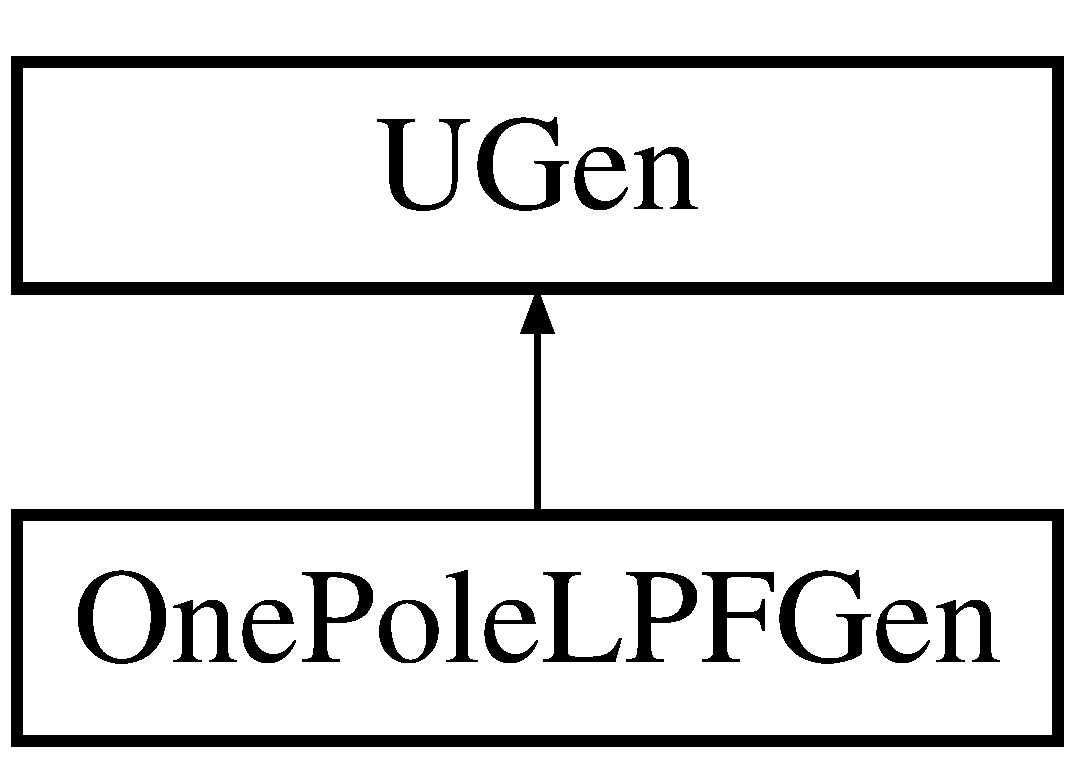
\includegraphics[height=2.000000cm]{classOnePoleLPFGen}
\end{center}
\end{figure}
\subsection*{Public Member Functions}
\begin{DoxyCompactItemize}
\item 
{\bfseries One\+Pole\+L\+P\+F\+Gen} (std\+::string name)\hypertarget{classOnePoleLPFGen_aea39a9562852ac47fdd576fd8b583b9f}{}\label{classOnePoleLPFGen_aea39a9562852ac47fdd576fd8b583b9f}

\item 
void {\bfseries control} (std\+::string port\+Name, float value)\hypertarget{classOnePoleLPFGen_a8f2df9b7406edadf7dc34e7e65b2b67c}{}\label{classOnePoleLPFGen_a8f2df9b7406edadf7dc34e7e65b2b67c}

\item 
float {\bfseries tick} ()\hypertarget{classOnePoleLPFGen_a5e5288841ff8112113f2d6ec1f03f375}{}\label{classOnePoleLPFGen_a5e5288841ff8112113f2d6ec1f03f375}

\end{DoxyCompactItemize}
\subsection*{Additional Inherited Members}


The documentation for this class was generated from the following files\+:\begin{DoxyCompactItemize}
\item 
unit/One\+Pole\+L\+P\+F\+Gen.\+h\item 
unit/One\+Pole\+L\+P\+F\+Gen.\+cpp\end{DoxyCompactItemize}

\hypertarget{classOscActivator}{}\section{Osc\+Activator Class Reference}
\label{classOscActivator}\index{Osc\+Activator@{Osc\+Activator}}
Inheritance diagram for Osc\+Activator\+:\begin{figure}[H]
\begin{center}
\leavevmode
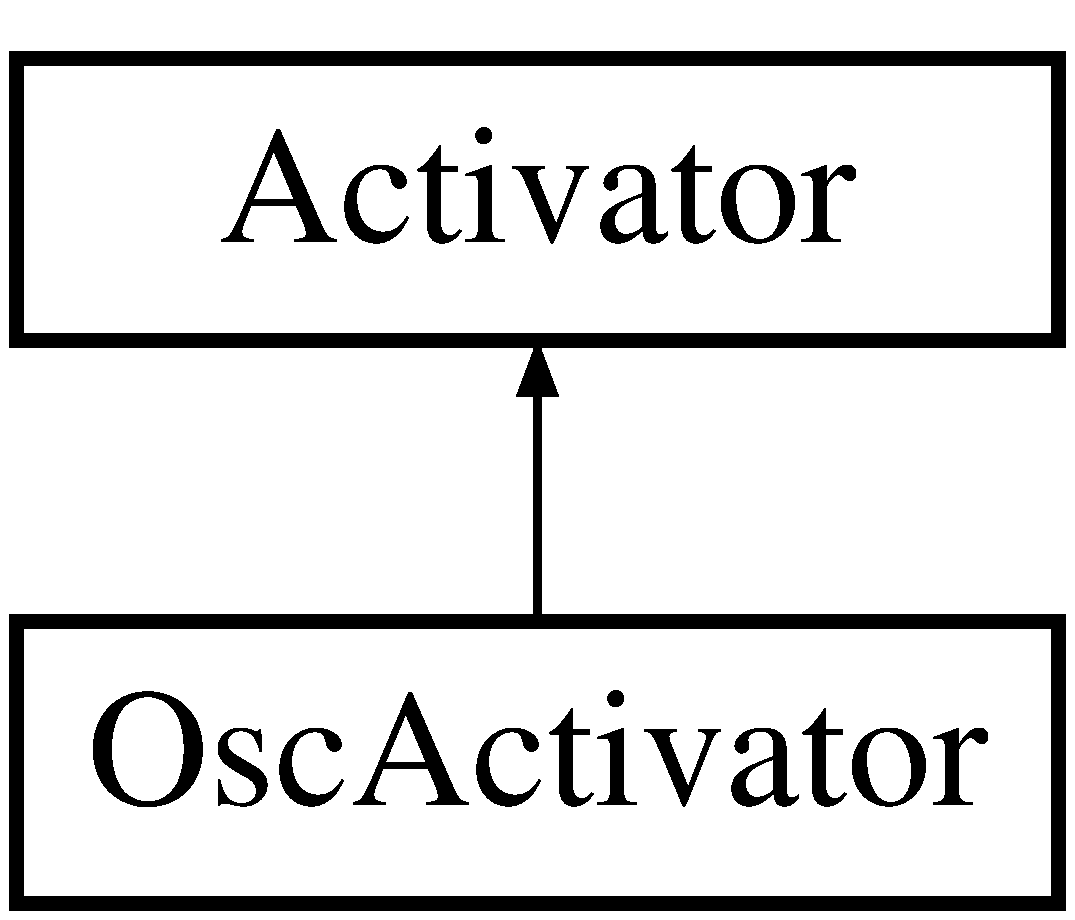
\includegraphics[height=2.000000cm]{classOscActivator}
\end{center}
\end{figure}
\subsection*{Public Member Functions}
\begin{DoxyCompactItemize}
\item 
void {\bfseries callback} (float value)\hypertarget{classOscActivator_ad5852376e949408b2fc13c8adf60c032}{}\label{classOscActivator_ad5852376e949408b2fc13c8adf60c032}

\end{DoxyCompactItemize}


The documentation for this class was generated from the following files\+:\begin{DoxyCompactItemize}
\item 
sequencer/Osc\+Activator.\+h\item 
sequencer/Osc\+Activator.\+cpp\end{DoxyCompactItemize}

\hypertarget{classOscInConnector}{}\section{Osc\+In\+Connector Class Reference}
\label{classOscInConnector}\index{Osc\+In\+Connector@{Osc\+In\+Connector}}
\subsection*{Classes}
\begin{DoxyCompactItemize}
\item 
class \hyperlink{classOscInConnector_1_1MidiPacketListener}{Midi\+Packet\+Listener}
\end{DoxyCompactItemize}
\subsection*{Public Member Functions}
\begin{DoxyCompactItemize}
\item 
{\bfseries Osc\+In\+Connector} (int prt)\hypertarget{classOscInConnector_acb8cca9cec941690ed0dcee6611c4553}{}\label{classOscInConnector_acb8cca9cec941690ed0dcee6611c4553}

\item 
bool {\bfseries is\+Fresh} ()\hypertarget{classOscInConnector_a6603048c9ba0e9356a8dd0f5ffc1055f}{}\label{classOscInConnector_a6603048c9ba0e9356a8dd0f5ffc1055f}

\item 
\hyperlink{classMessageData}{Message\+Data} $\ast$ {\bfseries get\+Data} ()\hypertarget{classOscInConnector_aa7130d46061b498d0f8648c0bd9c4146}{}\label{classOscInConnector_aa7130d46061b498d0f8648c0bd9c4146}

\item 
std\+::thread \hyperlink{classOscInConnector_af546d19cf2adc1ed7c701a4804586cb9}{start\+Thread} ()
\end{DoxyCompactItemize}
\subsection*{Public Attributes}
\begin{DoxyCompactItemize}
\item 
\hyperlink{classMessageData}{Message\+Data} $\ast$ {\bfseries MD} = new \hyperlink{classMessageData}{Message\+Data}(\char`\"{}xxx\char`\"{},1,2,3,3.\+14f)\hypertarget{classOscInConnector_a5ff52e9ac740d92aec0eb9f1eee00ddf}{}\label{classOscInConnector_a5ff52e9ac740d92aec0eb9f1eee00ddf}

\item 
bool {\bfseries talk} = true\hypertarget{classOscInConnector_a0472faba62d4db290aeb71326b31d5cc}{}\label{classOscInConnector_a0472faba62d4db290aeb71326b31d5cc}

\end{DoxyCompactItemize}


\subsection{Member Function Documentation}
\index{Osc\+In\+Connector@{Osc\+In\+Connector}!start\+Thread@{start\+Thread}}
\index{start\+Thread@{start\+Thread}!Osc\+In\+Connector@{Osc\+In\+Connector}}
\subsubsection[{\texorpdfstring{start\+Thread()}{startThread()}}]{\setlength{\rightskip}{0pt plus 5cm}std\+::thread Osc\+In\+Connector\+::start\+Thread (
\begin{DoxyParamCaption}
{}
\end{DoxyParamCaption}
)}\hypertarget{classOscInConnector_af546d19cf2adc1ed7c701a4804586cb9}{}\label{classOscInConnector_af546d19cf2adc1ed7c701a4804586cb9}
Scheint zu funktionieren, keine Ahnung warum \+:) 

The documentation for this class was generated from the following files\+:\begin{DoxyCompactItemize}
\item 
osc/Osc\+In\+Connector.\+h\item 
osc/Osc\+In\+Connector.\+cpp\end{DoxyCompactItemize}

\hypertarget{classOscOutConnector}{}\section{Osc\+Out\+Connector Class Reference}
\label{classOscOutConnector}\index{Osc\+Out\+Connector@{Osc\+Out\+Connector}}
\subsection*{Public Member Functions}
\begin{DoxyCompactItemize}
\item 
{\bfseries Osc\+Out\+Connector} (std\+::string h, int p)\hypertarget{classOscOutConnector_a7dde00203135c4a673e56f02dec774b4}{}\label{classOscOutConnector_a7dde00203135c4a673e56f02dec774b4}

\item 
void {\bfseries send\+Message} (std\+::string s, int a1, int a2, int a3, float f1)\hypertarget{classOscOutConnector_a8b3bcadf0295998b42753161ae9d17ee}{}\label{classOscOutConnector_a8b3bcadf0295998b42753161ae9d17ee}

\end{DoxyCompactItemize}


The documentation for this class was generated from the following files\+:\begin{DoxyCompactItemize}
\item 
Osc\+Out\+Connector.\+h\item 
Osc\+Out\+Connector.\+cpp\end{DoxyCompactItemize}

\hypertarget{classOscWrapper}{\section{Osc\-Wrapper Class Reference}
\label{classOscWrapper}\index{Osc\-Wrapper@{Osc\-Wrapper}}
}


The documentation for this class was generated from the following files\-:\begin{DoxyCompactItemize}
\item 
include/Osc\-Wrapper.\-h\item 
store/Osc\-Wrapper.\-cpp\end{DoxyCompactItemize}

\hypertarget{classPatch}{}\section{Patch Class Reference}
\label{classPatch}\index{Patch@{Patch}}
\subsection*{Public Member Functions}
\begin{DoxyCompactItemize}
\item 
{\bfseries Patch} (std\+::string from, int pt\+From, std\+::string to, int p\+To)\hypertarget{classPatch_a5ff9de0f83c44aa11aae837870aa55f0}{}\label{classPatch_a5ff9de0f83c44aa11aae837870aa55f0}

\item 
std\+::string {\bfseries get\+From} ()\hypertarget{classPatch_a97b08ef9e08c5ef8b5d71692a7242796}{}\label{classPatch_a97b08ef9e08c5ef8b5d71692a7242796}

\item 
int {\bfseries get\+From\+Port} ()\hypertarget{classPatch_a365988c401459bfd0f0b5b21f041bfe1}{}\label{classPatch_a365988c401459bfd0f0b5b21f041bfe1}

\item 
std\+::string {\bfseries get\+To} ()\hypertarget{classPatch_ade1fb3107faa8224f29c4a8387821fee}{}\label{classPatch_ade1fb3107faa8224f29c4a8387821fee}

\item 
int {\bfseries get\+Form\+Port} ()\hypertarget{classPatch_a19e489d67f86b80ac5f0ef774a3b87c8}{}\label{classPatch_a19e489d67f86b80ac5f0ef774a3b87c8}

\end{DoxyCompactItemize}


The documentation for this class was generated from the following files\+:\begin{DoxyCompactItemize}
\item 
unit/Patch.\+h\item 
unit/Patch.\+cpp\end{DoxyCompactItemize}

\hypertarget{classPhasorGen}{}\section{Phasor\+Gen Class Reference}
\label{classPhasorGen}\index{Phasor\+Gen@{Phasor\+Gen}}
Inheritance diagram for Phasor\+Gen\+:\begin{figure}[H]
\begin{center}
\leavevmode
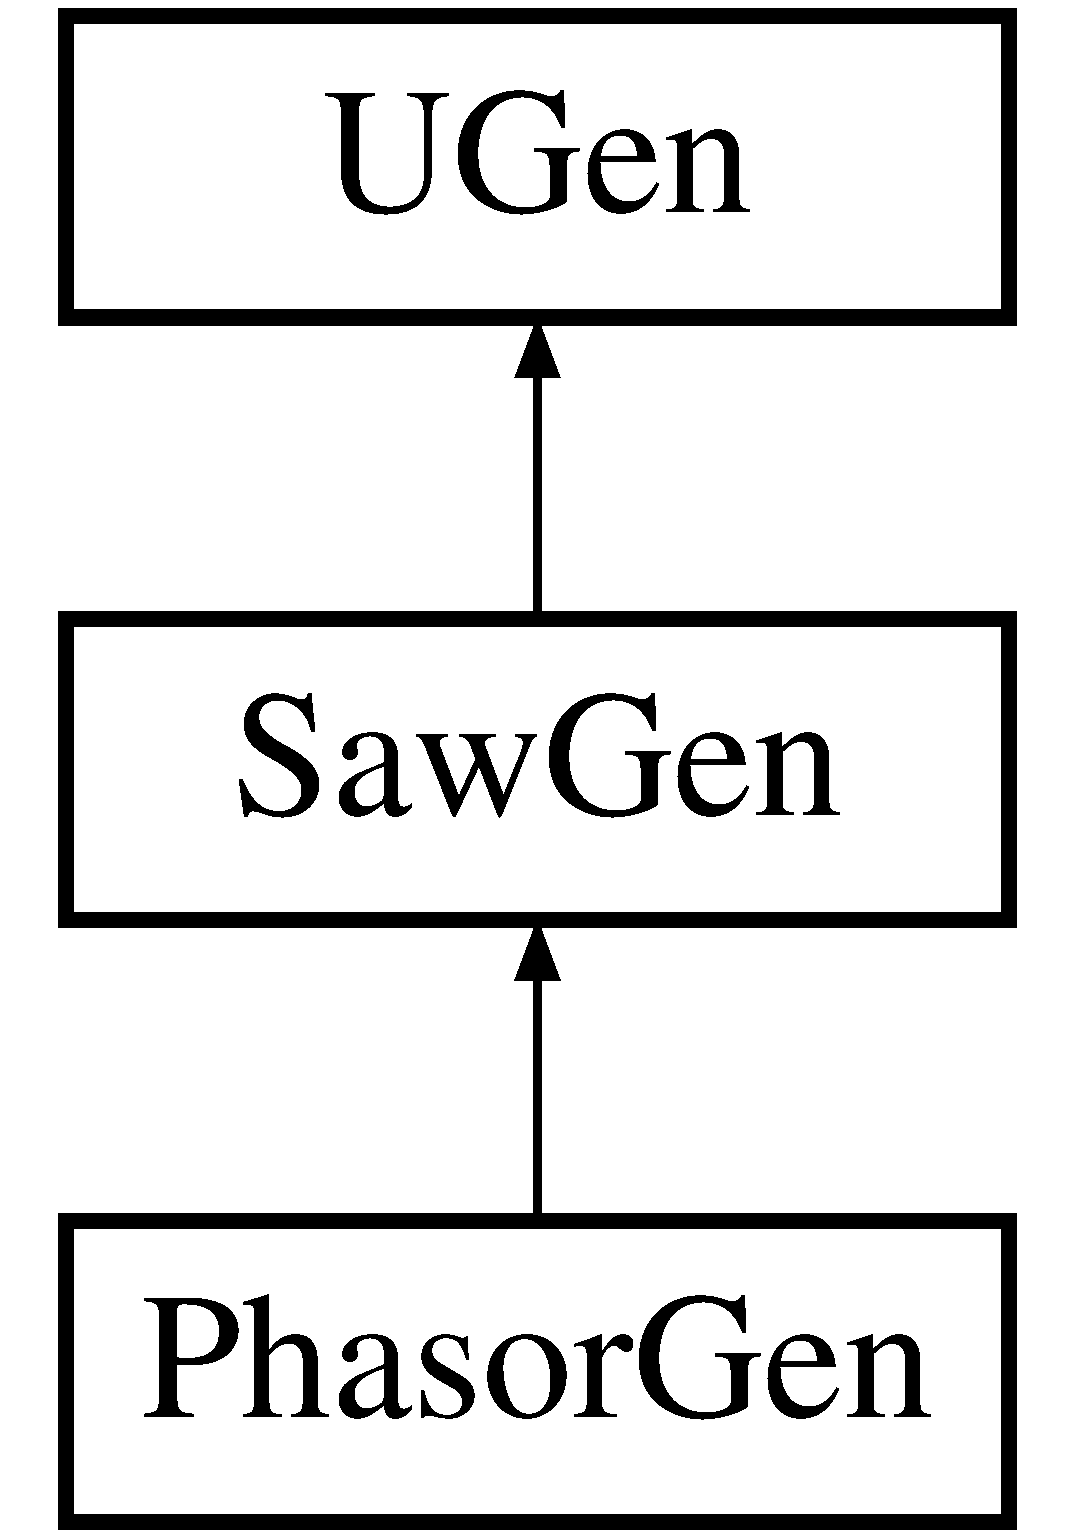
\includegraphics[height=3.000000cm]{classPhasorGen}
\end{center}
\end{figure}
\subsection*{Public Member Functions}
\begin{DoxyCompactItemize}
\item 
{\bfseries Phasor\+Gen} (std\+::string name)\hypertarget{classPhasorGen_a726fab6730e45d7fbf242f4613837e28}{}\label{classPhasorGen_a726fab6730e45d7fbf242f4613837e28}

\item 
float {\bfseries tick} ()\hypertarget{classPhasorGen_a056953090628af9868e4778d15daf79a}{}\label{classPhasorGen_a056953090628af9868e4778d15daf79a}

\end{DoxyCompactItemize}
\subsection*{Additional Inherited Members}


The documentation for this class was generated from the following files\+:\begin{DoxyCompactItemize}
\item 
unit/Phasor\+Gen.\+h\item 
unit/Phasor\+Gen.\+cpp\end{DoxyCompactItemize}

\hypertarget{classPort}{\section{Port Class Reference}
\label{classPort}\index{Port@{Port}}
}
\subsection*{Public Member Functions}
\begin{DoxyCompactItemize}
\item 
\hypertarget{classPort_aadff8efe873e31b3362dda2b4a28c8c9}{{\bfseries Port} (std\-::string name, Port\-Type t)}\label{classPort_aadff8efe873e31b3362dda2b4a28c8c9}

\item 
\hypertarget{classPort_ad2c3baf0b291aee3b5b65178231754a6}{std\-::string {\bfseries get\-Name} ()}\label{classPort_ad2c3baf0b291aee3b5b65178231754a6}

\item 
\hypertarget{classPort_a31744528a5ade68a59ce094f3797bc1e}{std\-::string {\bfseries get\-I\-D} ()}\label{classPort_a31744528a5ade68a59ce094f3797bc1e}

\item 
\hypertarget{classPort_a5859f5d788d56c0103f4274b6d62b725}{Port\-Type {\bfseries get\-Type} ()}\label{classPort_a5859f5d788d56c0103f4274b6d62b725}

\item 
\hypertarget{classPort_a101b9cfba62777fb61c35a642b63f25a}{float {\bfseries get\-Value} ()}\label{classPort_a101b9cfba62777fb61c35a642b63f25a}

\item 
\hypertarget{classPort_afc93a217ba756e559c157b66745823a7}{void {\bfseries set\-Value} (float v)}\label{classPort_afc93a217ba756e559c157b66745823a7}

\end{DoxyCompactItemize}


The documentation for this class was generated from the following files\-:\begin{DoxyCompactItemize}
\item 
src/include/Port.\-h\item 
src/unit/Port.\-cpp\end{DoxyCompactItemize}

\hypertarget{classPulse}{\section{Pulse Class Reference}
\label{classPulse}\index{Pulse@{Pulse}}
}


{\ttfamily \#include $<$Pulse.\-h$>$}

\subsection*{Public Member Functions}
\begin{DoxyCompactItemize}
\item 
\hypertarget{classPulse_a9835b637db766732dd508c94fc30c501}{{\bfseries Pulse} (float bpm)}\label{classPulse_a9835b637db766732dd508c94fc30c501}

\item 
\hypertarget{classPulse_a164d81d4e1e798a5eec15b0b030b4047}{void {\bfseries start} ()}\label{classPulse_a164d81d4e1e798a5eec15b0b030b4047}

\item 
\hypertarget{classPulse_a7c8121986bec5319bb097216fe5e93d0}{void {\bfseries stop} ()}\label{classPulse_a7c8121986bec5319bb097216fe5e93d0}

\item 
\hypertarget{classPulse_a8283f4ab252e0c38b1e19a4dec522f23}{void {\bfseries set\-Activator} (\hyperlink{classActivator}{Activator} $\ast$a)}\label{classPulse_a8283f4ab252e0c38b1e19a4dec522f23}

\item 
\hypertarget{classPulse_afc87b2e4120c47942cf03fc82aaf8002}{void {\bfseries set\-Speed} (float bpm)}\label{classPulse_afc87b2e4120c47942cf03fc82aaf8002}

\end{DoxyCompactItemize}


\subsection{Detailed Description}
\hyperlink{classPulse}{Pulse} generates a beat and sends the pulses to an \hyperlink{classActivator}{Activator}. The pulse is quantized to a zweiundreissigstel (thirty second note/demisemiquaver).

\begin{DoxyAuthor}{Author}
jtm, email\-:  \href{mailto:milde@hs-fulda.de}{\tt milde@hs-\/fulda.\-de} 
\end{DoxyAuthor}
\begin{DoxySince}{Since}
04-\/2016 
\end{DoxySince}
\begin{DoxyVersion}{Version}
1.\-0 
\end{DoxyVersion}


The documentation for this class was generated from the following files\-:\begin{DoxyCompactItemize}
\item 
include/Pulse.\-h\item 
sequencer/Pulse.\-cpp\end{DoxyCompactItemize}

\hypertarget{classSawGen}{}\section{Saw\+Gen Class Reference}
\label{classSawGen}\index{Saw\+Gen@{Saw\+Gen}}
Inheritance diagram for Saw\+Gen\+:\begin{figure}[H]
\begin{center}
\leavevmode
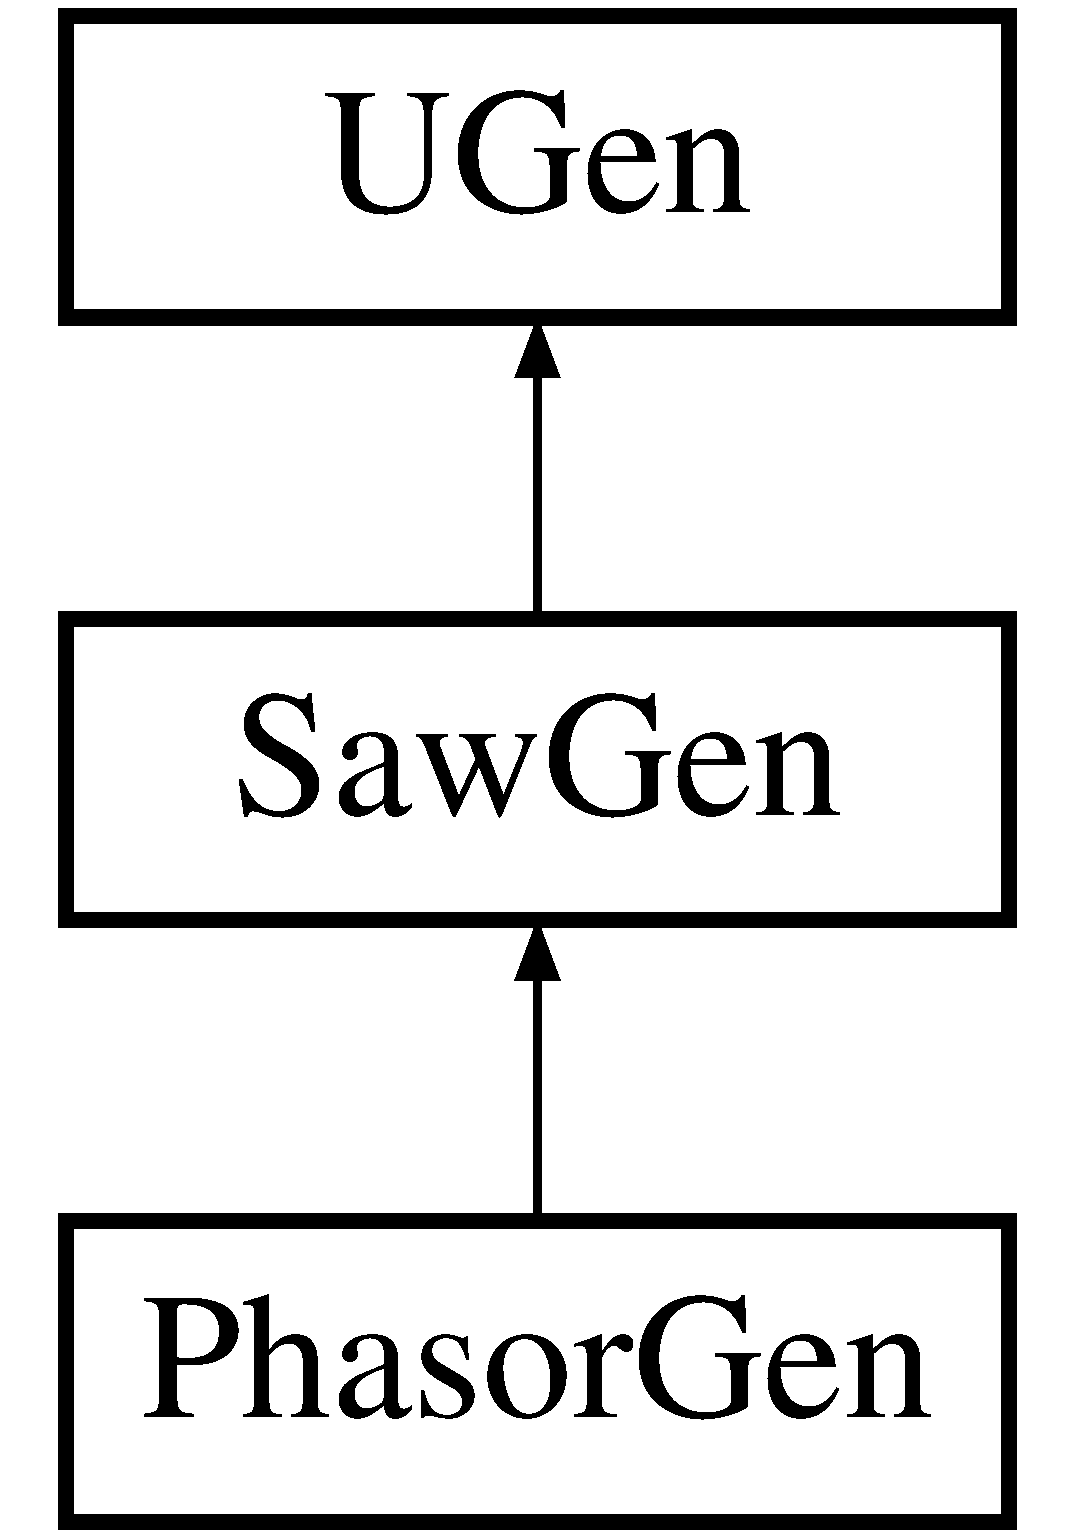
\includegraphics[height=3.000000cm]{classSawGen}
\end{center}
\end{figure}
\subsection*{Public Member Functions}
\begin{DoxyCompactItemize}
\item 
{\bfseries Saw\+Gen} (std\+::string name)\hypertarget{classSawGen_a24c35afc1bdb237a8a5d1eb3888ce0bc}{}\label{classSawGen_a24c35afc1bdb237a8a5d1eb3888ce0bc}

\item 
void {\bfseries control} (std\+::string port\+Name, float value)\hypertarget{classSawGen_a515f6eb82a1a97ee434144b8c58133b8}{}\label{classSawGen_a515f6eb82a1a97ee434144b8c58133b8}

\item 
float {\bfseries tick} ()\hypertarget{classSawGen_a18c6704aec8f20a5605ff72d674c7516}{}\label{classSawGen_a18c6704aec8f20a5605ff72d674c7516}

\end{DoxyCompactItemize}
\subsection*{Additional Inherited Members}


The documentation for this class was generated from the following files\+:\begin{DoxyCompactItemize}
\item 
unit/Saw\+Gen.\+h\item 
unit/Saw\+Gen.\+cpp\end{DoxyCompactItemize}

\hypertarget{classSoundUnit}{}\section{Sound\+Unit Class Reference}
\label{classSoundUnit}\index{Sound\+Unit@{Sound\+Unit}}
Inheritance diagram for Sound\+Unit\+:\begin{figure}[H]
\begin{center}
\leavevmode
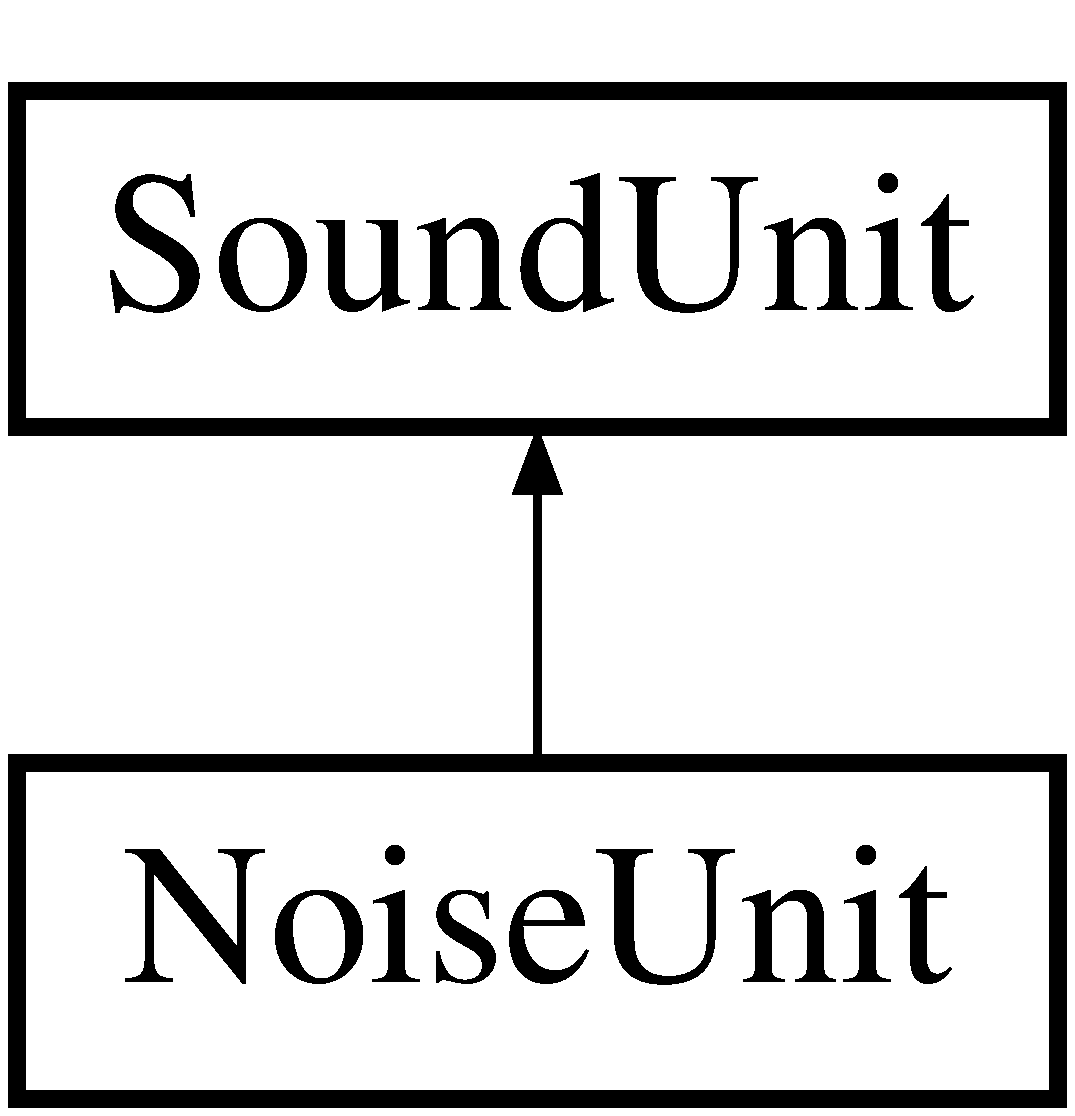
\includegraphics[height=2.000000cm]{classSoundUnit}
\end{center}
\end{figure}
\subsection*{Public Member Functions}
\begin{DoxyCompactItemize}
\item 
{\bfseries Sound\+Unit} (std\+::string name)\hypertarget{classSoundUnit_a3220665fe1e433d1b0d90fa328e71133}{}\label{classSoundUnit_a3220665fe1e433d1b0d90fa328e71133}

\item 
void {\bfseries add\+U\+Gen} (\hyperlink{classUGen}{U\+Gen} $\ast$u)\hypertarget{classSoundUnit_ab88bf7e7dfb77cf7e18587fd5a637755}{}\label{classSoundUnit_ab88bf7e7dfb77cf7e18587fd5a637755}

\item 
std\+::string {\bfseries get\+Name} ()\hypertarget{classSoundUnit_a4854dfb9b839ff33d061ed013fbf3ef9}{}\label{classSoundUnit_a4854dfb9b839ff33d061ed013fbf3ef9}

\item 
virtual void {\bfseries setup} ()=0\hypertarget{classSoundUnit_aedfa9b99f4555ed5df4ceffe001c1e63}{}\label{classSoundUnit_aedfa9b99f4555ed5df4ceffe001c1e63}

\item 
virtual void {\bfseries control} (std\+::string port\+Name, float value)=0\hypertarget{classSoundUnit_a0a74ef3d6c9343f1ee64a9a96bdbbe78}{}\label{classSoundUnit_a0a74ef3d6c9343f1ee64a9a96bdbbe78}

\item 
virtual float {\bfseries tick} ()=0\hypertarget{classSoundUnit_af1f6ccffb8d1919bd774b340c01bea68}{}\label{classSoundUnit_af1f6ccffb8d1919bd774b340c01bea68}

\end{DoxyCompactItemize}
\subsection*{Protected Attributes}
\begin{DoxyCompactItemize}
\item 
std\+::map$<$ std\+::string, \hyperlink{classUGen}{U\+Gen} $\ast$ $>$ {\bfseries U\+G\+E\+NS}\hypertarget{classSoundUnit_aa7bb4be0804fdd7a68bd767795592da1}{}\label{classSoundUnit_aa7bb4be0804fdd7a68bd767795592da1}

\end{DoxyCompactItemize}


The documentation for this class was generated from the following files\+:\begin{DoxyCompactItemize}
\item 
unit/Sound\+Unit.\+h\item 
unit/Sound\+Unit.\+cpp\end{DoxyCompactItemize}

\hypertarget{classSquareGen}{}\section{Square\+Gen Class Reference}
\label{classSquareGen}\index{Square\+Gen@{Square\+Gen}}
Inheritance diagram for Square\+Gen\+:\begin{figure}[H]
\begin{center}
\leavevmode
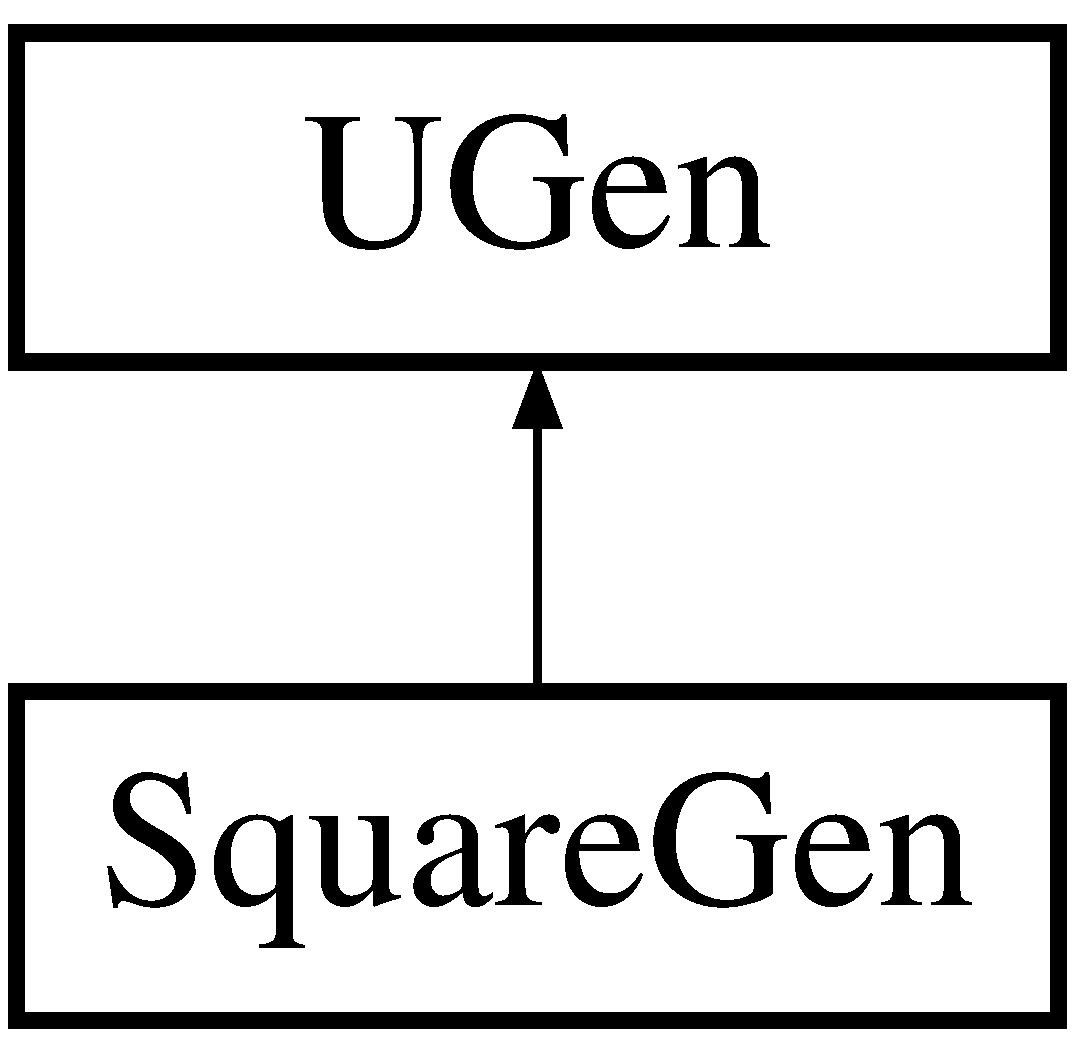
\includegraphics[height=2.000000cm]{classSquareGen}
\end{center}
\end{figure}
\subsection*{Public Member Functions}
\begin{DoxyCompactItemize}
\item 
{\bfseries Square\+Gen} (std\+::string name)\hypertarget{classSquareGen_a626505e8ade08b9383acda8901aa23b5}{}\label{classSquareGen_a626505e8ade08b9383acda8901aa23b5}

\item 
void {\bfseries control} (std\+::string port\+Name, float value)\hypertarget{classSquareGen_a8a25dc2b8c5d1ec7857e4da7ec96cecc}{}\label{classSquareGen_a8a25dc2b8c5d1ec7857e4da7ec96cecc}

\item 
float {\bfseries tick} ()\hypertarget{classSquareGen_a119ab47582ee5814687b87db6a71644c}{}\label{classSquareGen_a119ab47582ee5814687b87db6a71644c}

\end{DoxyCompactItemize}
\subsection*{Additional Inherited Members}


The documentation for this class was generated from the following files\+:\begin{DoxyCompactItemize}
\item 
unit/Square\+Gen.\+h\item 
unit/Square\+Gen.\+cpp\end{DoxyCompactItemize}

\hypertarget{classSTKAdapterGen}{}\section{S\+T\+K\+Adapter\+Gen Class Reference}
\label{classSTKAdapterGen}\index{S\+T\+K\+Adapter\+Gen@{S\+T\+K\+Adapter\+Gen}}
Inheritance diagram for S\+T\+K\+Adapter\+Gen\+:\begin{figure}[H]
\begin{center}
\leavevmode
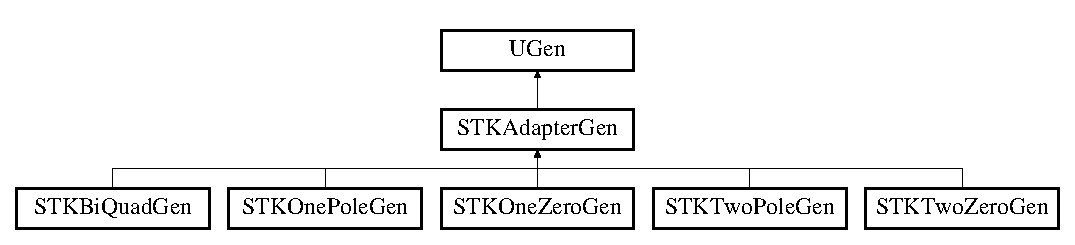
\includegraphics[height=2.847458cm]{classSTKAdapterGen}
\end{center}
\end{figure}
\subsection*{Additional Inherited Members}


The documentation for this class was generated from the following file\+:\begin{DoxyCompactItemize}
\item 
unit/S\+T\+K\+Adapter\+Gen.\+h\end{DoxyCompactItemize}

\hypertarget{classSTKBiQuadGen}{}\section{S\+T\+K\+Bi\+Quad\+Gen Class Reference}
\label{classSTKBiQuadGen}\index{S\+T\+K\+Bi\+Quad\+Gen@{S\+T\+K\+Bi\+Quad\+Gen}}
Inheritance diagram for S\+T\+K\+Bi\+Quad\+Gen\+:\begin{figure}[H]
\begin{center}
\leavevmode
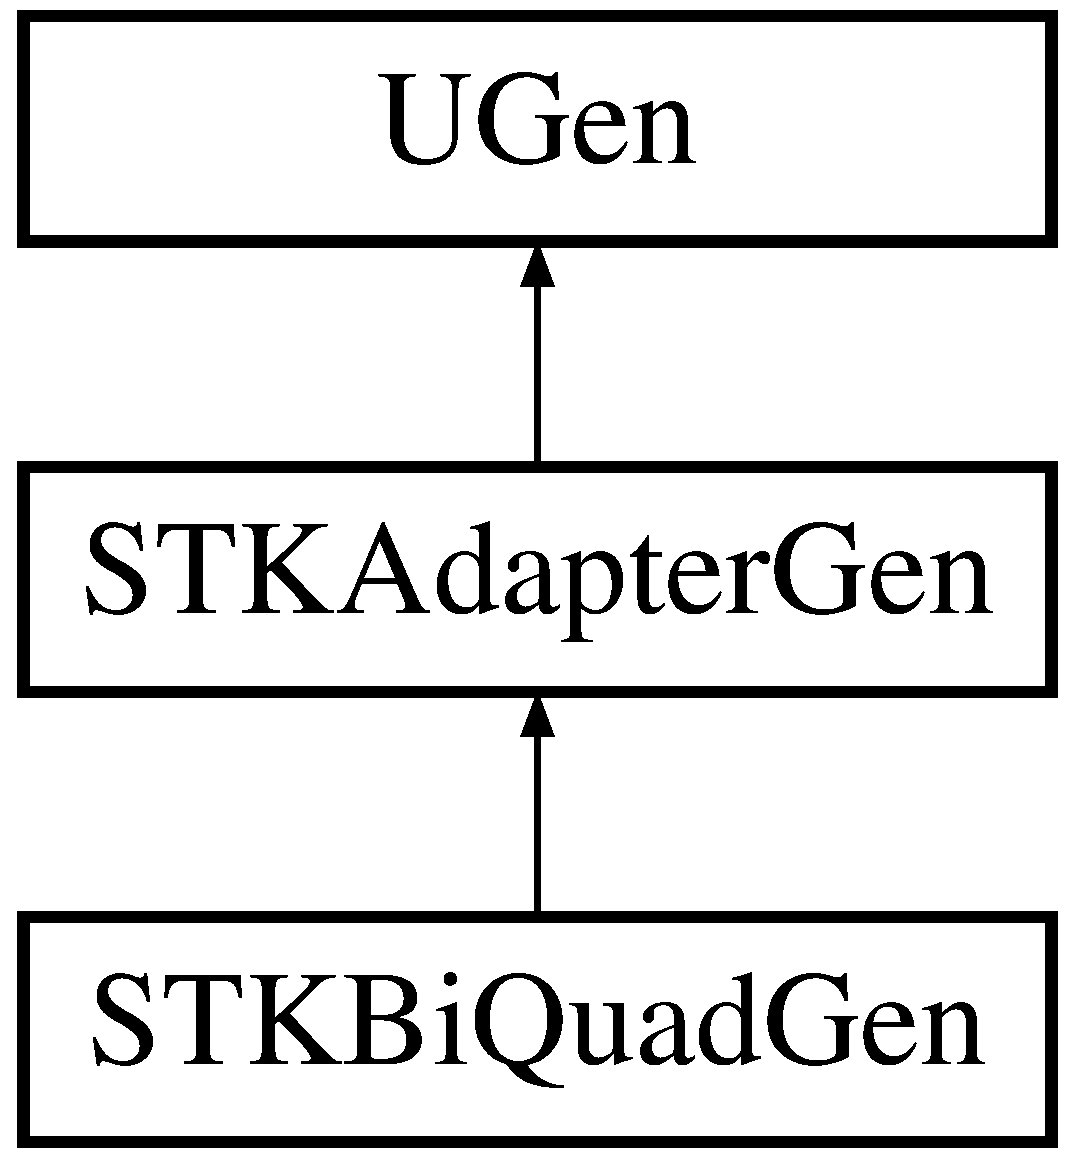
\includegraphics[height=3.000000cm]{classSTKBiQuadGen}
\end{center}
\end{figure}
\subsection*{Public Member Functions}
\begin{DoxyCompactItemize}
\item 
void {\bfseries control} (std\+::string port\+Name, float value)\hypertarget{classSTKBiQuadGen_afbaea4e23ab453fdeaa0069ddd8002a6}{}\label{classSTKBiQuadGen_afbaea4e23ab453fdeaa0069ddd8002a6}

\item 
float {\bfseries tick} ()\hypertarget{classSTKBiQuadGen_aeaa64c8ff587d9a9089b4cf3276255b9}{}\label{classSTKBiQuadGen_aeaa64c8ff587d9a9089b4cf3276255b9}

\end{DoxyCompactItemize}
\subsection*{Additional Inherited Members}


The documentation for this class was generated from the following files\+:\begin{DoxyCompactItemize}
\item 
unit/S\+T\+K\+Bi\+Quad\+Gen.\+h\item 
unit/S\+T\+K\+Bi\+Quad\+Gen.\+cpp\end{DoxyCompactItemize}

\hypertarget{classSTKOnePoleGen}{}\section{S\+T\+K\+One\+Pole\+Gen Class Reference}
\label{classSTKOnePoleGen}\index{S\+T\+K\+One\+Pole\+Gen@{S\+T\+K\+One\+Pole\+Gen}}
Inheritance diagram for S\+T\+K\+One\+Pole\+Gen\+:\begin{figure}[H]
\begin{center}
\leavevmode
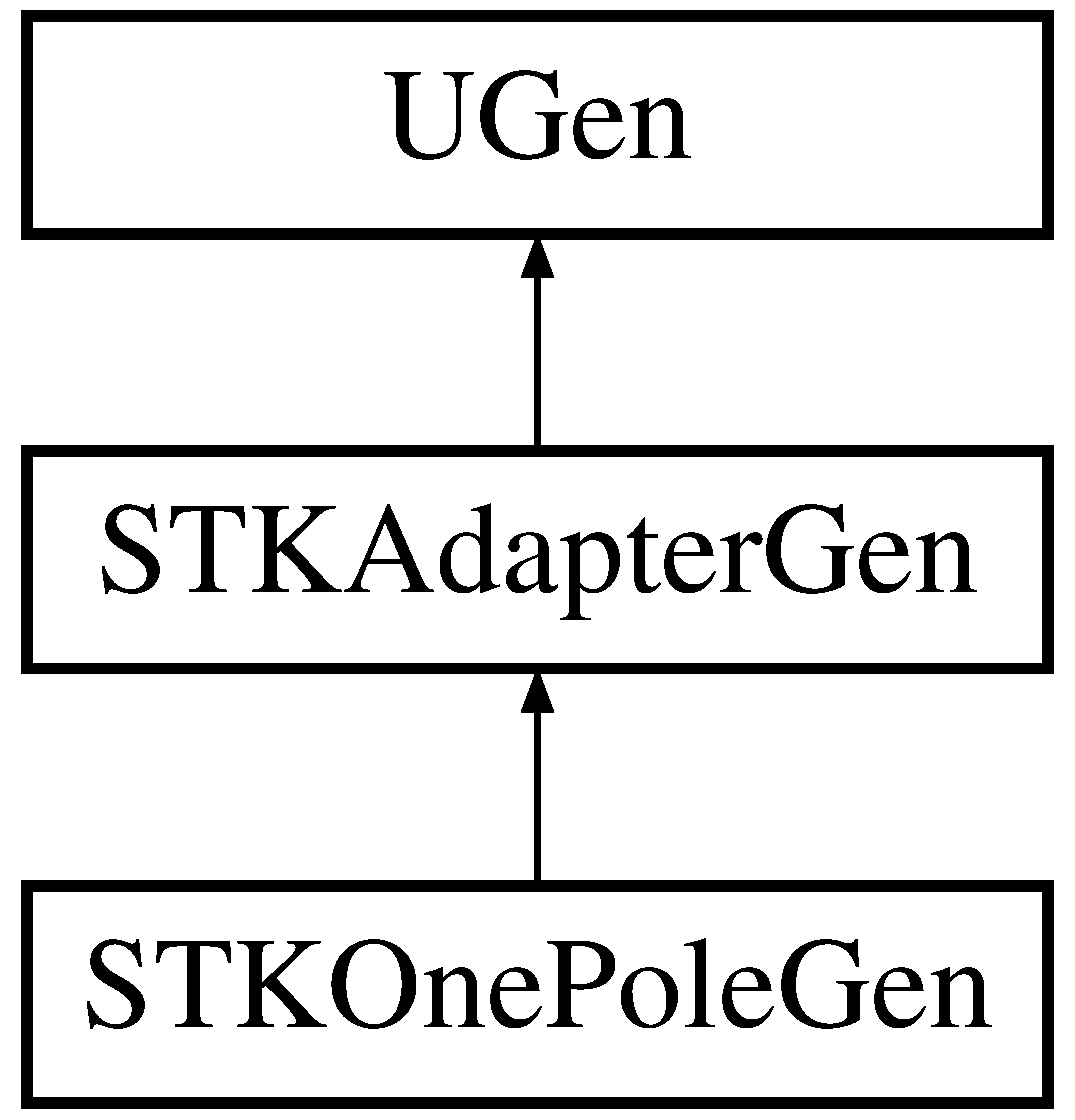
\includegraphics[height=3.000000cm]{classSTKOnePoleGen}
\end{center}
\end{figure}
\subsection*{Public Member Functions}
\begin{DoxyCompactItemize}
\item 
void {\bfseries control} (std\+::string port\+Name, float value)\hypertarget{classSTKOnePoleGen_abafc7a64770438cbde61518a7cf2d94b}{}\label{classSTKOnePoleGen_abafc7a64770438cbde61518a7cf2d94b}

\item 
float {\bfseries tick} ()\hypertarget{classSTKOnePoleGen_a3bc702fbc334d94eebd409755d1d74e8}{}\label{classSTKOnePoleGen_a3bc702fbc334d94eebd409755d1d74e8}

\end{DoxyCompactItemize}
\subsection*{Additional Inherited Members}


The documentation for this class was generated from the following files\+:\begin{DoxyCompactItemize}
\item 
unit/S\+T\+K\+One\+Pole\+Gen.\+h\item 
unit/S\+T\+K\+One\+Pole\+Gen.\+cpp\end{DoxyCompactItemize}

\hypertarget{classSTKOneZeroGen}{}\section{S\+T\+K\+One\+Zero\+Gen Class Reference}
\label{classSTKOneZeroGen}\index{S\+T\+K\+One\+Zero\+Gen@{S\+T\+K\+One\+Zero\+Gen}}
Inheritance diagram for S\+T\+K\+One\+Zero\+Gen\+:\begin{figure}[H]
\begin{center}
\leavevmode
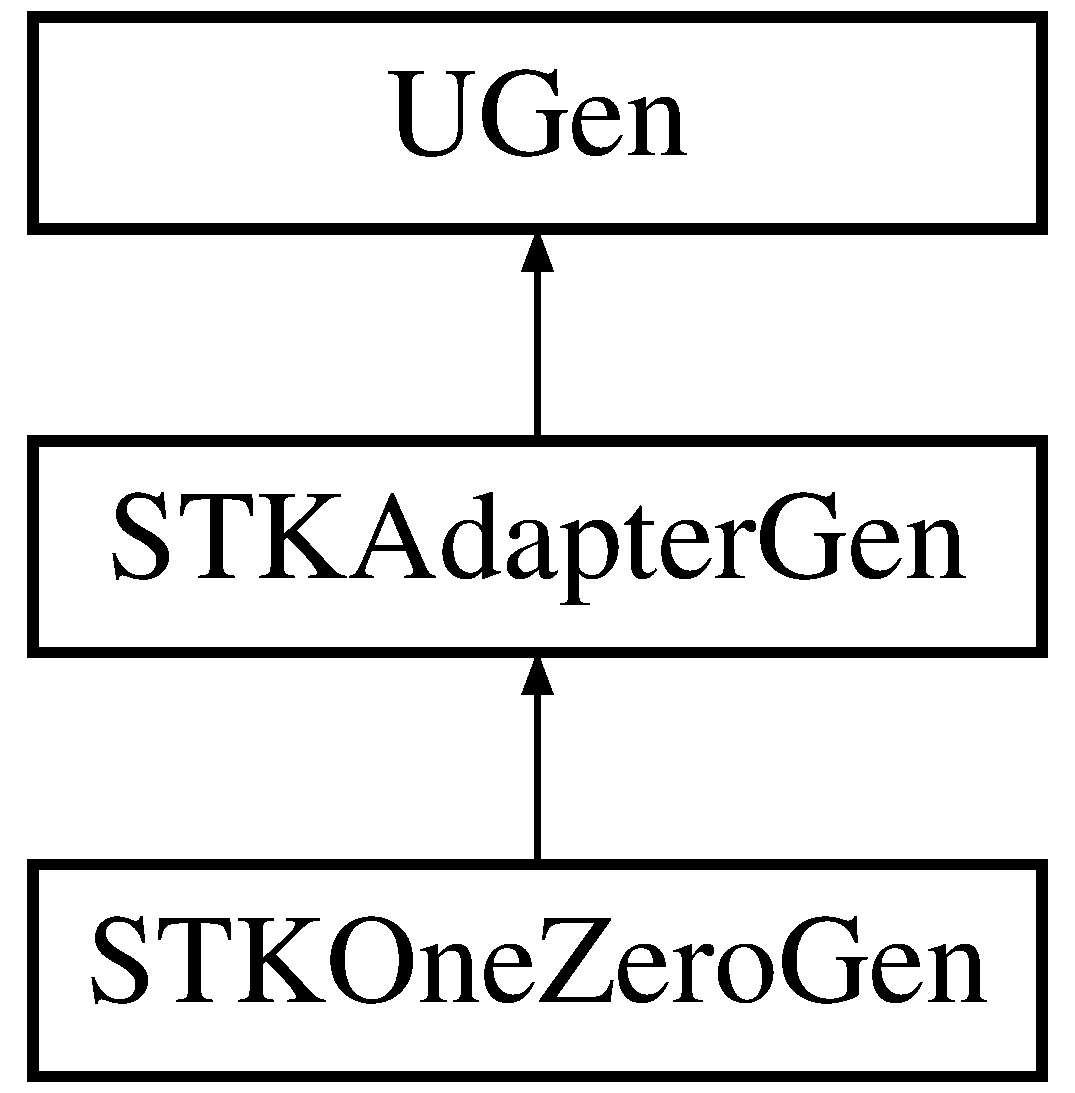
\includegraphics[height=3.000000cm]{classSTKOneZeroGen}
\end{center}
\end{figure}
\subsection*{Public Member Functions}
\begin{DoxyCompactItemize}
\item 
void {\bfseries control} (std\+::string port\+Name, float value)\hypertarget{classSTKOneZeroGen_a44bc26cf6f0e7218f9f14447c957dce4}{}\label{classSTKOneZeroGen_a44bc26cf6f0e7218f9f14447c957dce4}

\item 
float {\bfseries tick} ()\hypertarget{classSTKOneZeroGen_ab1118ea13c6892f49c8f92f017b82908}{}\label{classSTKOneZeroGen_ab1118ea13c6892f49c8f92f017b82908}

\end{DoxyCompactItemize}
\subsection*{Additional Inherited Members}


The documentation for this class was generated from the following files\+:\begin{DoxyCompactItemize}
\item 
unit/S\+T\+K\+One\+Zero\+Gen.\+h\item 
unit/S\+T\+K\+One\+Zero\+Gen.\+cpp\end{DoxyCompactItemize}

\hypertarget{classSTKTwoPoleGen}{}\section{S\+T\+K\+Two\+Pole\+Gen Class Reference}
\label{classSTKTwoPoleGen}\index{S\+T\+K\+Two\+Pole\+Gen@{S\+T\+K\+Two\+Pole\+Gen}}
Inheritance diagram for S\+T\+K\+Two\+Pole\+Gen\+:\begin{figure}[H]
\begin{center}
\leavevmode
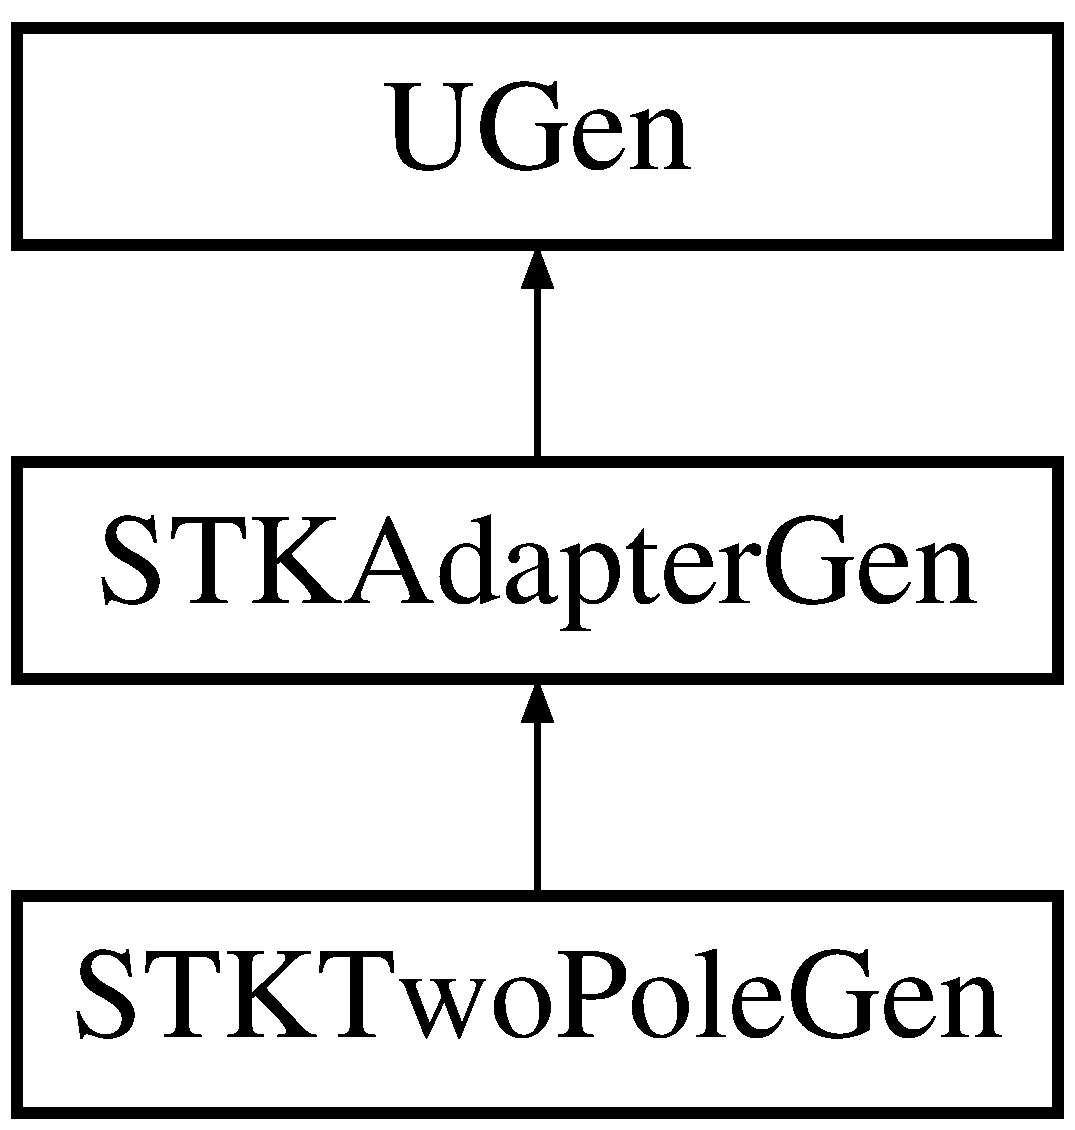
\includegraphics[height=3.000000cm]{classSTKTwoPoleGen}
\end{center}
\end{figure}
\subsection*{Public Member Functions}
\begin{DoxyCompactItemize}
\item 
void {\bfseries control} (std\+::string port\+Name, float value)\hypertarget{classSTKTwoPoleGen_a71b904b3c03c69f5fb25bbf2449fb802}{}\label{classSTKTwoPoleGen_a71b904b3c03c69f5fb25bbf2449fb802}

\item 
float {\bfseries tick} ()\hypertarget{classSTKTwoPoleGen_ade033932ab7e85b7f3d6a69461eef372}{}\label{classSTKTwoPoleGen_ade033932ab7e85b7f3d6a69461eef372}

\end{DoxyCompactItemize}
\subsection*{Additional Inherited Members}


The documentation for this class was generated from the following files\+:\begin{DoxyCompactItemize}
\item 
unit/S\+T\+K\+Two\+Pole\+Gen.\+h\item 
unit/S\+T\+K\+Two\+Pole\+Gen.\+cpp\end{DoxyCompactItemize}

\hypertarget{classSTKTwoZeroGen}{}\section{S\+T\+K\+Two\+Zero\+Gen Class Reference}
\label{classSTKTwoZeroGen}\index{S\+T\+K\+Two\+Zero\+Gen@{S\+T\+K\+Two\+Zero\+Gen}}
Inheritance diagram for S\+T\+K\+Two\+Zero\+Gen\+:\begin{figure}[H]
\begin{center}
\leavevmode
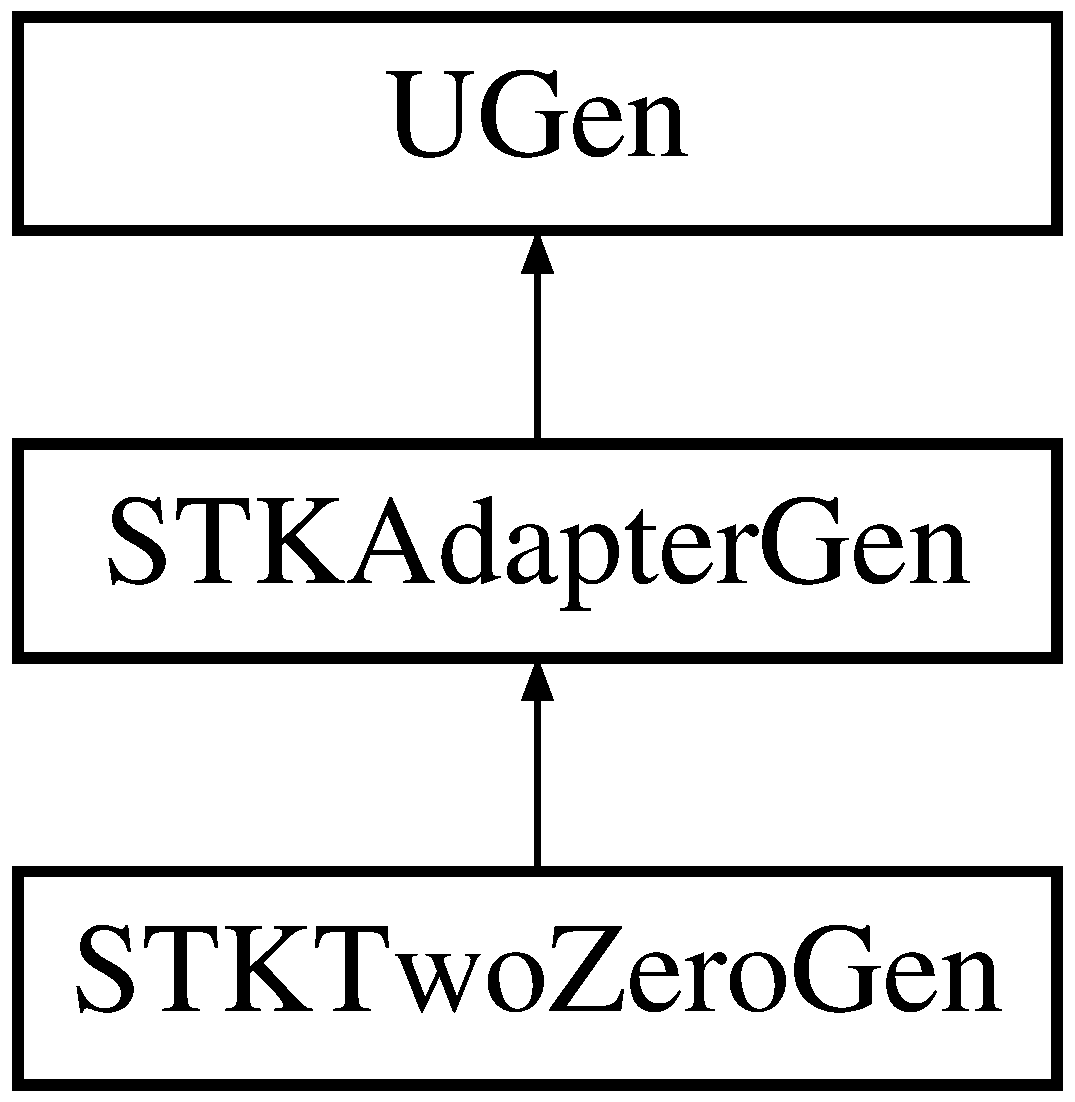
\includegraphics[height=3.000000cm]{classSTKTwoZeroGen}
\end{center}
\end{figure}
\subsection*{Public Member Functions}
\begin{DoxyCompactItemize}
\item 
void {\bfseries control} (std\+::string port\+Name, float value)\hypertarget{classSTKTwoZeroGen_a35f0458e31142985a3f35b603ff90e62}{}\label{classSTKTwoZeroGen_a35f0458e31142985a3f35b603ff90e62}

\item 
float {\bfseries tick} ()\hypertarget{classSTKTwoZeroGen_a1e9392a2e8dc67862de802e914acbf33}{}\label{classSTKTwoZeroGen_a1e9392a2e8dc67862de802e914acbf33}

\end{DoxyCompactItemize}
\subsection*{Additional Inherited Members}


The documentation for this class was generated from the following files\+:\begin{DoxyCompactItemize}
\item 
unit/S\+T\+K\+Two\+Zero\+Gen.\+h\item 
unit/S\+T\+K\+Two\+Zero\+Gen.\+cpp\end{DoxyCompactItemize}

\hypertarget{classTestStatic}{\section{Test\-Static Class Reference}
\label{classTestStatic}\index{Test\-Static@{Test\-Static}}
}
\subsection*{Public Member Functions}
\begin{DoxyCompactItemize}
\item 
\hypertarget{classTestStatic_af877b62beba36ec427f5a20cf0b261e5}{void {\bfseries printit} ()}\label{classTestStatic_af877b62beba36ec427f5a20cf0b261e5}

\end{DoxyCompactItemize}
\subsection*{Static Public Member Functions}
\begin{DoxyCompactItemize}
\item 
\hypertarget{classTestStatic_af09e079b702a6fba0a9623c136665d90}{static void {\bfseries do\-Something} (int val)}\label{classTestStatic_af09e079b702a6fba0a9623c136665d90}

\end{DoxyCompactItemize}


The documentation for this class was generated from the following files\-:\begin{DoxyCompactItemize}
\item 
src/outdated/Test\-Static.\-h\item 
src/outdated/Test\-Static.\-cpp\end{DoxyCompactItemize}

\hypertarget{structTickData}{\section{Tick\-Data Struct Reference}
\label{structTickData}\index{Tick\-Data@{Tick\-Data}}
}
\subsection*{Public Attributes}
\begin{DoxyCompactItemize}
\item 
\hypertarget{structTickData_a81bc42e25163a7afb9725153fac3d713}{stk\-::\-Stk\-Float {\bfseries volume}}\label{structTickData_a81bc42e25163a7afb9725153fac3d713}

\item 
\hypertarget{structTickData_a9916301f9f675256327e1ac0bdb8f9f4}{stk\-::\-Stk\-Float {\bfseries t60}}\label{structTickData_a9916301f9f675256327e1ac0bdb8f9f4}

\item 
\hypertarget{structTickData_abda86f5671f18f3e09fa6e0877c70bca}{unsigned int {\bfseries n\-Wv\-Outs}}\label{structTickData_abda86f5671f18f3e09fa6e0877c70bca}

\item 
\hypertarget{structTickData_ac53a7ecd6dfff24019bfb607202f6024}{int {\bfseries n\-Voices}}\label{structTickData_ac53a7ecd6dfff24019bfb607202f6024}

\item 
\hypertarget{structTickData_a620ca81cff77e4cdaf0025b73bc37e61}{int {\bfseries current\-Voice}}\label{structTickData_a620ca81cff77e4cdaf0025b73bc37e61}

\item 
\hypertarget{structTickData_ad147869433dc1b3526aa9f4dbb3b4cc5}{int {\bfseries channels}}\label{structTickData_ad147869433dc1b3526aa9f4dbb3b4cc5}

\item 
\hypertarget{structTickData_a54ba17f6bb83ce8efe0758614221f026}{int {\bfseries counter}}\label{structTickData_a54ba17f6bb83ce8efe0758614221f026}

\item 
\hypertarget{structTickData_aa60016ecb88b0bdae8395aa7517a6f1f}{bool {\bfseries realtime}}\label{structTickData_aa60016ecb88b0bdae8395aa7517a6f1f}

\item 
\hypertarget{structTickData_a4682f375c65eb79d9166933ec9c79c2b}{bool {\bfseries settling}}\label{structTickData_a4682f375c65eb79d9166933ec9c79c2b}

\item 
\hypertarget{structTickData_a142d947db0ab6e66f8f912c51a4bafdb}{bool {\bfseries have\-Message}}\label{structTickData_a142d947db0ab6e66f8f912c51a4bafdb}

\item 
\hypertarget{structTickData_ade8d551a52ad93b8f056bf5da813c64c}{int {\bfseries frequency}}\label{structTickData_ade8d551a52ad93b8f056bf5da813c64c}

\item 
\hypertarget{structTickData_a99559444aee6dbc126f650744c5487ec}{Wv\-Out $\ast$$\ast$ {\bfseries wvout}}\label{structTickData_a99559444aee6dbc126f650744c5487ec}

\item 
\hypertarget{structTickData_aa2b6f7f6ad9c886711e9393aca979677}{Instrmnt $\ast$$\ast$ {\bfseries instrument}}\label{structTickData_aa2b6f7f6ad9c886711e9393aca979677}

\item 
\hypertarget{structTickData_ade98160894388bc8534d2003a7a63ffe}{Voicer $\ast$ {\bfseries voicer}}\label{structTickData_ade98160894388bc8534d2003a7a63ffe}

\item 
\hypertarget{structTickData_a3d1563b3668509206700be3e02138827}{J\-C\-Rev {\bfseries reverb}}\label{structTickData_a3d1563b3668509206700be3e02138827}

\item 
\hypertarget{structTickData_a3d0c2a9deef2fd2bd94b3ba8c6b176eb}{Messager {\bfseries messager}}\label{structTickData_a3d0c2a9deef2fd2bd94b3ba8c6b176eb}

\item 
\hypertarget{structTickData_a3061482937dae6c292d4d51400a6143a}{Skini\-::\-Message {\bfseries message}}\label{structTickData_a3061482937dae6c292d4d51400a6143a}

\item 
\hypertarget{structTickData_a6d0680a0bcc9d2c35104ad9721777223}{Stk\-Float {\bfseries volume}}\label{structTickData_a6d0680a0bcc9d2c35104ad9721777223}

\item 
\hypertarget{structTickData_adf8ffe69c6880e995aec842a032ee9fe}{Stk\-Float {\bfseries t60}}\label{structTickData_adf8ffe69c6880e995aec842a032ee9fe}

\end{DoxyCompactItemize}


The documentation for this struct was generated from the following files\-:\begin{DoxyCompactItemize}
\item 
include/Tick\-Data.\-h\item 
outdated/first.\-cpp\end{DoxyCompactItemize}

\hypertarget{classTwoInputMixerGen}{}\section{Two\+Input\+Mixer\+Gen Class Reference}
\label{classTwoInputMixerGen}\index{Two\+Input\+Mixer\+Gen@{Two\+Input\+Mixer\+Gen}}
Inheritance diagram for Two\+Input\+Mixer\+Gen\+:\begin{figure}[H]
\begin{center}
\leavevmode
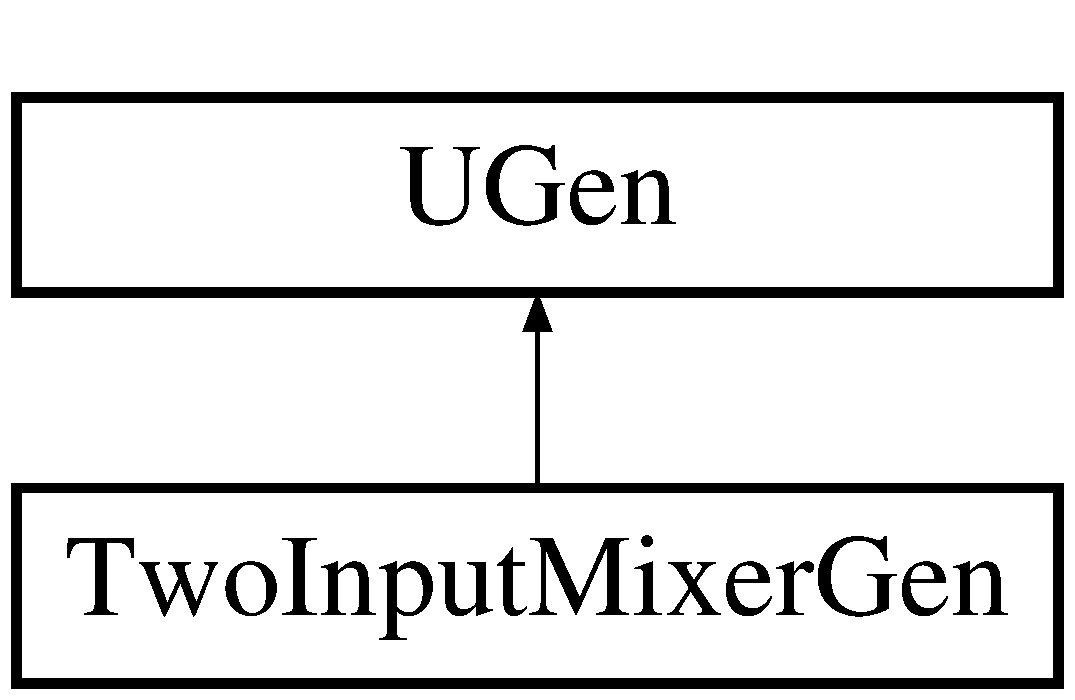
\includegraphics[height=2.000000cm]{classTwoInputMixerGen}
\end{center}
\end{figure}
\subsection*{Public Member Functions}
\begin{DoxyCompactItemize}
\item 
{\bfseries Two\+Input\+Mixer\+Gen} (std\+::string name)\hypertarget{classTwoInputMixerGen_ae150f51a934ffb7330f8a2852b094539}{}\label{classTwoInputMixerGen_ae150f51a934ffb7330f8a2852b094539}

\item 
float {\bfseries tick} ()\hypertarget{classTwoInputMixerGen_aef96ef6828e767384a8881d108c0d52b}{}\label{classTwoInputMixerGen_aef96ef6828e767384a8881d108c0d52b}

\item 
void {\bfseries control} (std\+::string port\+Name, float value)\hypertarget{classTwoInputMixerGen_ab8d7d00eb0c692a8c2de706f58673d3d}{}\label{classTwoInputMixerGen_ab8d7d00eb0c692a8c2de706f58673d3d}

\end{DoxyCompactItemize}
\subsection*{Additional Inherited Members}


The documentation for this class was generated from the following files\+:\begin{DoxyCompactItemize}
\item 
unit/Two\+Input\+Mixer\+Gen.\+h\item 
unit/Two\+Input\+Mixer\+Gen.\+cpp\end{DoxyCompactItemize}

\hypertarget{classUGen}{}\section{U\+Gen Class Reference}
\label{classUGen}\index{U\+Gen@{U\+Gen}}
Inheritance diagram for U\+Gen\+:\begin{figure}[H]
\begin{center}
\leavevmode
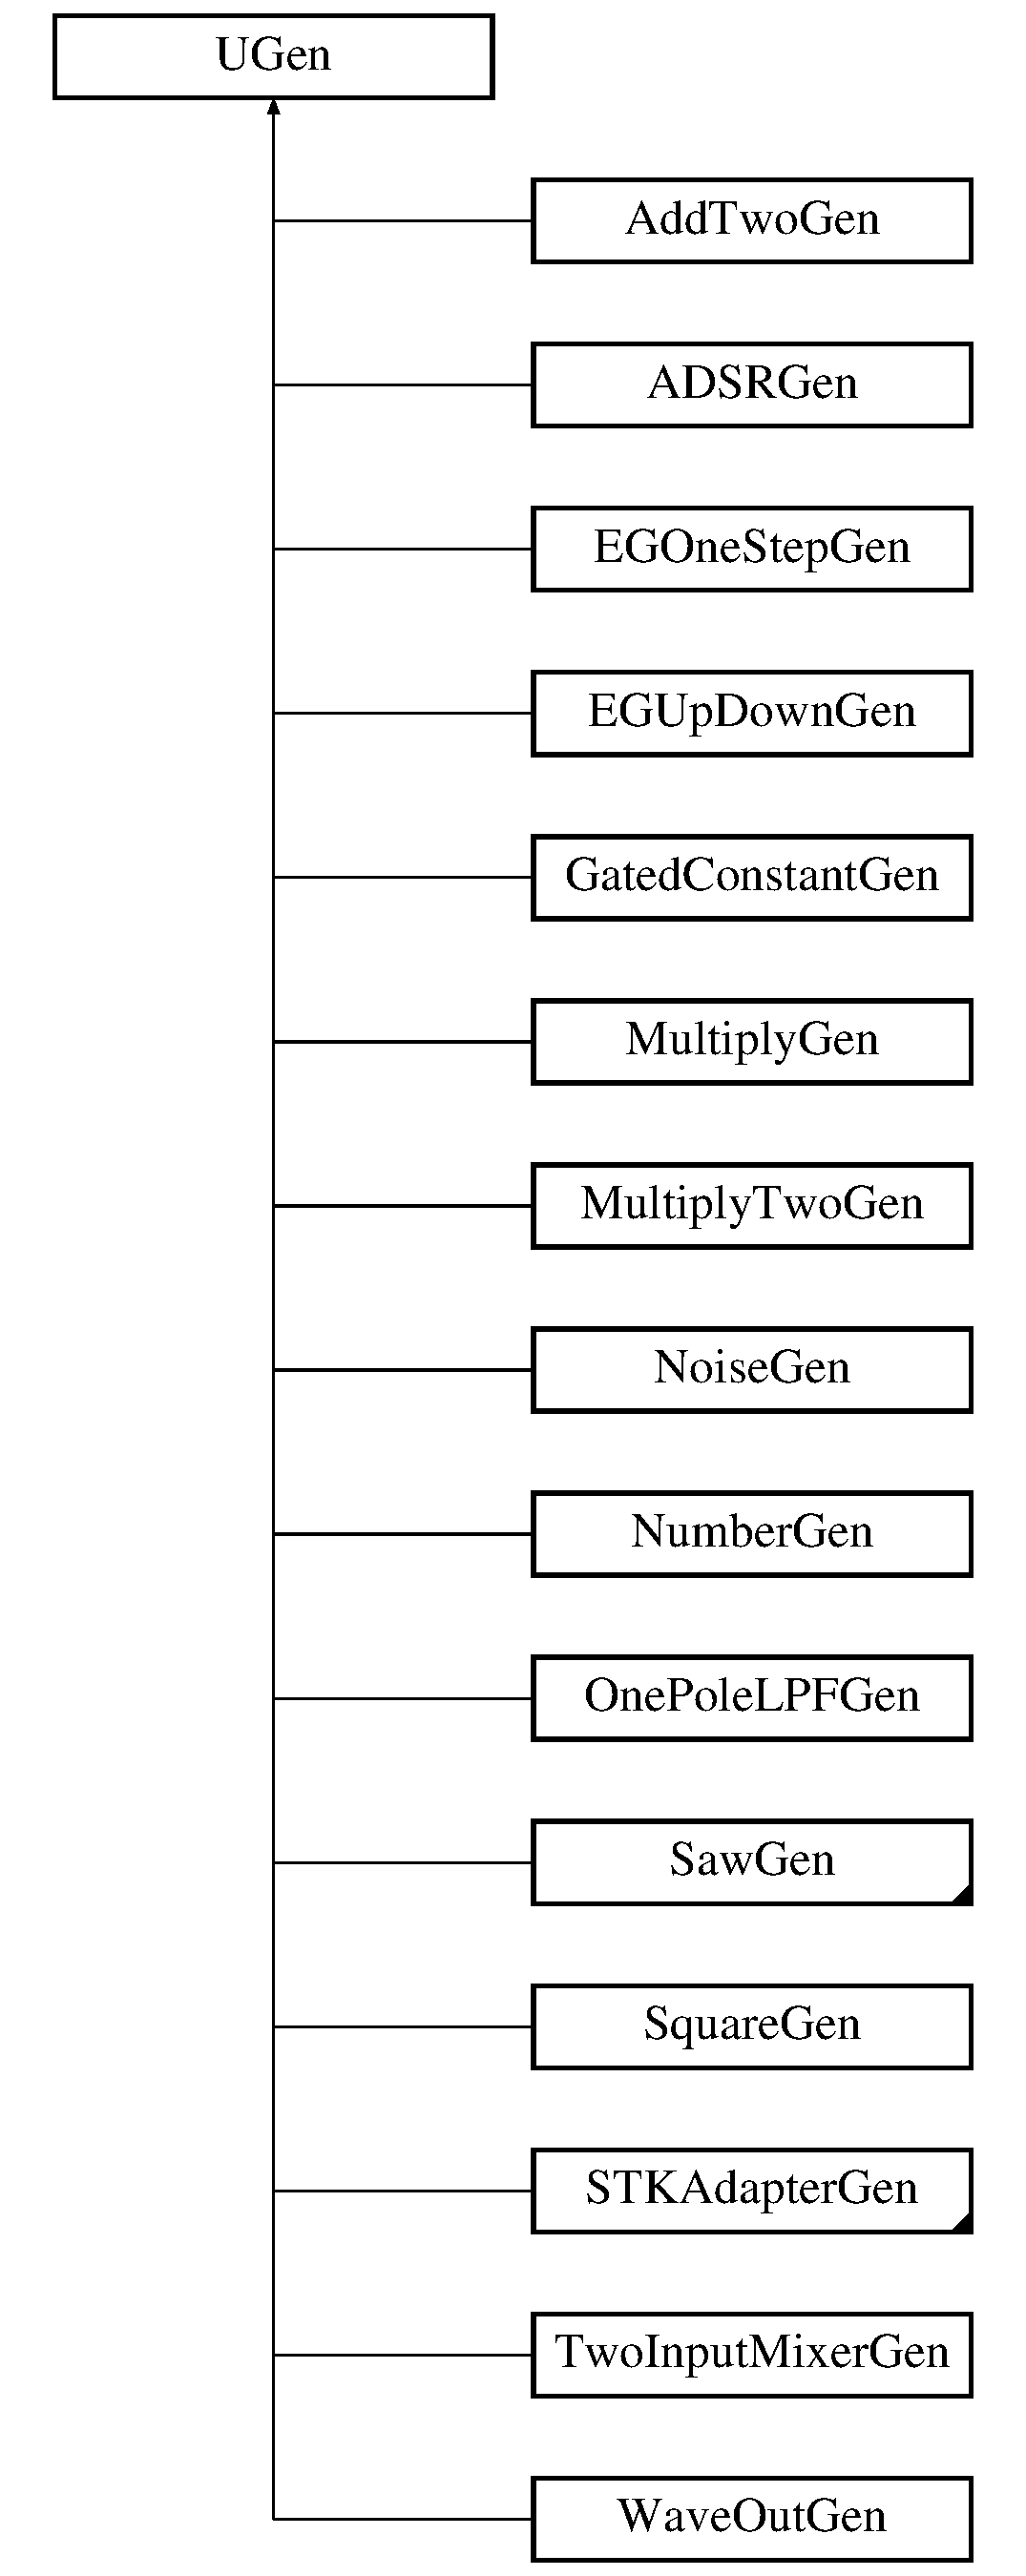
\includegraphics[height=12.000000cm]{classUGen}
\end{center}
\end{figure}
\subsection*{Public Member Functions}
\begin{DoxyCompactItemize}
\item 
{\bfseries U\+Gen} (std\+::string name, int pn)\hypertarget{classUGen_af2d6d70e1340c9853a9a329cb2db164a}{}\label{classUGen_af2d6d70e1340c9853a9a329cb2db164a}

\item 
void {\bfseries add\+Port} (\hyperlink{classPort}{Port} p)\hypertarget{classUGen_a7d5be76c0847cea2ffd9fb6118dad84b}{}\label{classUGen_a7d5be76c0847cea2ffd9fb6118dad84b}

\item 
\hyperlink{classPort}{Port} $\ast$ {\bfseries get\+Ports} ()\hypertarget{classUGen_a2dbed70294dba960bebb4e6e6196f93f}{}\label{classUGen_a2dbed70294dba960bebb4e6e6196f93f}

\item 
int {\bfseries get\+Number\+Of\+Ports} ()\hypertarget{classUGen_a1f7c0151b63c89a92ea7b3b598969fb5}{}\label{classUGen_a1f7c0151b63c89a92ea7b3b598969fb5}

\item 
float {\bfseries get\+Port\+Value} (int pn)\hypertarget{classUGen_a5790d6f5f741d9286e12f27eafd86bd5}{}\label{classUGen_a5790d6f5f741d9286e12f27eafd86bd5}

\item 
float {\bfseries get\+Port\+Value} (std\+::string name)\hypertarget{classUGen_a2a33803a853db61cc79cc6da90ce511d}{}\label{classUGen_a2a33803a853db61cc79cc6da90ce511d}

\item 
void {\bfseries set\+Port\+Value} (int pn, float value)\hypertarget{classUGen_ae933825c4201f13cb481d399de1bd4d5}{}\label{classUGen_ae933825c4201f13cb481d399de1bd4d5}

\item 
void {\bfseries set\+Port\+Value} (std\+::string name, float value)\hypertarget{classUGen_a1ed212c207052705c9fbd2fb64fe1092}{}\label{classUGen_a1ed212c207052705c9fbd2fb64fe1092}

\item 
int {\bfseries get\+Port\+Index} (std\+::string id)\hypertarget{classUGen_a7caac30e931fe2e39c53be9a084e2709}{}\label{classUGen_a7caac30e931fe2e39c53be9a084e2709}

\item 
std\+::string {\bfseries get\+Name} ()\hypertarget{classUGen_adfb82e003597ca4876f803f0395b28d6}{}\label{classUGen_adfb82e003597ca4876f803f0395b28d6}

\item 
std\+::string {\bfseries get\+ID} ()\hypertarget{classUGen_a500ba300703167f4daa52b51841edf24}{}\label{classUGen_a500ba300703167f4daa52b51841edf24}

\item 
virtual void {\bfseries control} (std\+::string port\+Name, float value)\hypertarget{classUGen_a456a55e23a073bc77135525be38ad0eb}{}\label{classUGen_a456a55e23a073bc77135525be38ad0eb}

\item 
virtual float {\bfseries tick} ()\hypertarget{classUGen_a7fe124a01b35094197816cb8aa033c55}{}\label{classUGen_a7fe124a01b35094197816cb8aa033c55}

\item 
void {\bfseries set\+Amnt1} (float value)\hypertarget{classUGen_a5063e6854f054cf7870abf1fdcbf8e30}{}\label{classUGen_a5063e6854f054cf7870abf1fdcbf8e30}

\item 
float {\bfseries get\+Amnt1} ()\hypertarget{classUGen_a98614bdc04b7c096fa7a75e486898947}{}\label{classUGen_a98614bdc04b7c096fa7a75e486898947}

\item 
void {\bfseries set\+Amnt2} (float value)\hypertarget{classUGen_a13494a4d13ad1fd32d16d5d22c22fb6d}{}\label{classUGen_a13494a4d13ad1fd32d16d5d22c22fb6d}

\item 
float {\bfseries get\+Amnt2} ()\hypertarget{classUGen_aa051f663b3fd0568eae2cad11b69058c}{}\label{classUGen_aa051f663b3fd0568eae2cad11b69058c}

\item 
void {\bfseries set\+Amnt3} (float value)\hypertarget{classUGen_aad0a3b7250c400216930062d651a1cf4}{}\label{classUGen_aad0a3b7250c400216930062d651a1cf4}

\item 
float {\bfseries get\+Amnt3} ()\hypertarget{classUGen_ac884f3a8cd1886698a9e2745940b9e1a}{}\label{classUGen_ac884f3a8cd1886698a9e2745940b9e1a}

\item 
void {\bfseries set\+In1} (float value)\hypertarget{classUGen_a4c68a850f5a690e39fd3903e52da313a}{}\label{classUGen_a4c68a850f5a690e39fd3903e52da313a}

\item 
float {\bfseries get\+In1} ()\hypertarget{classUGen_af1f157f807936bd22e201c9fa67ff80e}{}\label{classUGen_af1f157f807936bd22e201c9fa67ff80e}

\item 
void {\bfseries set\+In2} (float value)\hypertarget{classUGen_af3307a09f1ccefb80804f85edc9e305d}{}\label{classUGen_af3307a09f1ccefb80804f85edc9e305d}

\item 
float {\bfseries get\+In2} ()\hypertarget{classUGen_a9860c88b35b1d9e66559501f196a861c}{}\label{classUGen_a9860c88b35b1d9e66559501f196a861c}

\item 
void {\bfseries set\+Out1} (float value)\hypertarget{classUGen_ad1746a0b6380906d0d4a004e5c169247}{}\label{classUGen_ad1746a0b6380906d0d4a004e5c169247}

\item 
float {\bfseries get\+Out1} ()\hypertarget{classUGen_a71c193b988474251015828825e7cb49e}{}\label{classUGen_a71c193b988474251015828825e7cb49e}

\item 
void {\bfseries set\+Out2} (float value)\hypertarget{classUGen_af23d4016474b7d88cbbb6ed6660a10db}{}\label{classUGen_af23d4016474b7d88cbbb6ed6660a10db}

\item 
float {\bfseries get\+Out2} ()\hypertarget{classUGen_a37c67120e26ba5eef873e3ceb775eea0}{}\label{classUGen_a37c67120e26ba5eef873e3ceb775eea0}

\end{DoxyCompactItemize}
\subsection*{Protected Attributes}
\begin{DoxyCompactItemize}
\item 
float {\bfseries S\+A\+M\+P\+L\+I\+N\+G\+\_\+\+F\+R\+E\+Q\+U\+E\+N\+CY} = 44100\hypertarget{classUGen_a0db8d2e9778b5d9f093eefcbdc2c9d89}{}\label{classUGen_a0db8d2e9778b5d9f093eefcbdc2c9d89}

\item 
float {\bfseries amnt1}\hypertarget{classUGen_ae858237d38f3cc95144b64fa047ac37b}{}\label{classUGen_ae858237d38f3cc95144b64fa047ac37b}

\item 
float {\bfseries amnt2}\hypertarget{classUGen_aa2e389fc2267db7843209f2a21fe8b43}{}\label{classUGen_aa2e389fc2267db7843209f2a21fe8b43}

\item 
float {\bfseries amnt3}\hypertarget{classUGen_a05da12719a925b3e73467a82ed410b10}{}\label{classUGen_a05da12719a925b3e73467a82ed410b10}

\item 
float {\bfseries in1}\hypertarget{classUGen_a6633122030153c6685c6b654b7c45974}{}\label{classUGen_a6633122030153c6685c6b654b7c45974}

\item 
float {\bfseries in2}\hypertarget{classUGen_acbb0ab4228fbfbe61f4dffd022303d52}{}\label{classUGen_acbb0ab4228fbfbe61f4dffd022303d52}

\item 
float {\bfseries out1}\hypertarget{classUGen_ad347230d1fca8ba33d8ee9f64bfb73cc}{}\label{classUGen_ad347230d1fca8ba33d8ee9f64bfb73cc}

\item 
float {\bfseries out2}\hypertarget{classUGen_a27053388a03f59fc135af48bab560d2c}{}\label{classUGen_a27053388a03f59fc135af48bab560d2c}

\item 
std\+::string {\bfseries N\+A\+ME}\hypertarget{classUGen_aa1bdc53d037fbcc73c52d7bf92a1064e}{}\label{classUGen_aa1bdc53d037fbcc73c52d7bf92a1064e}

\item 
std\+::string {\bfseries ID}\hypertarget{classUGen_a1e26df186fdde33f8b3c84c97f92db2e}{}\label{classUGen_a1e26df186fdde33f8b3c84c97f92db2e}

\end{DoxyCompactItemize}


The documentation for this class was generated from the following files\+:\begin{DoxyCompactItemize}
\item 
unit/U\+Gen.\+h\item 
unit/U\+Gen.\+cpp\end{DoxyCompactItemize}

\hypertarget{classWaveOutGen}{}\section{Wave\+Out\+Gen Class Reference}
\label{classWaveOutGen}\index{Wave\+Out\+Gen@{Wave\+Out\+Gen}}
Inheritance diagram for Wave\+Out\+Gen\+:\begin{figure}[H]
\begin{center}
\leavevmode
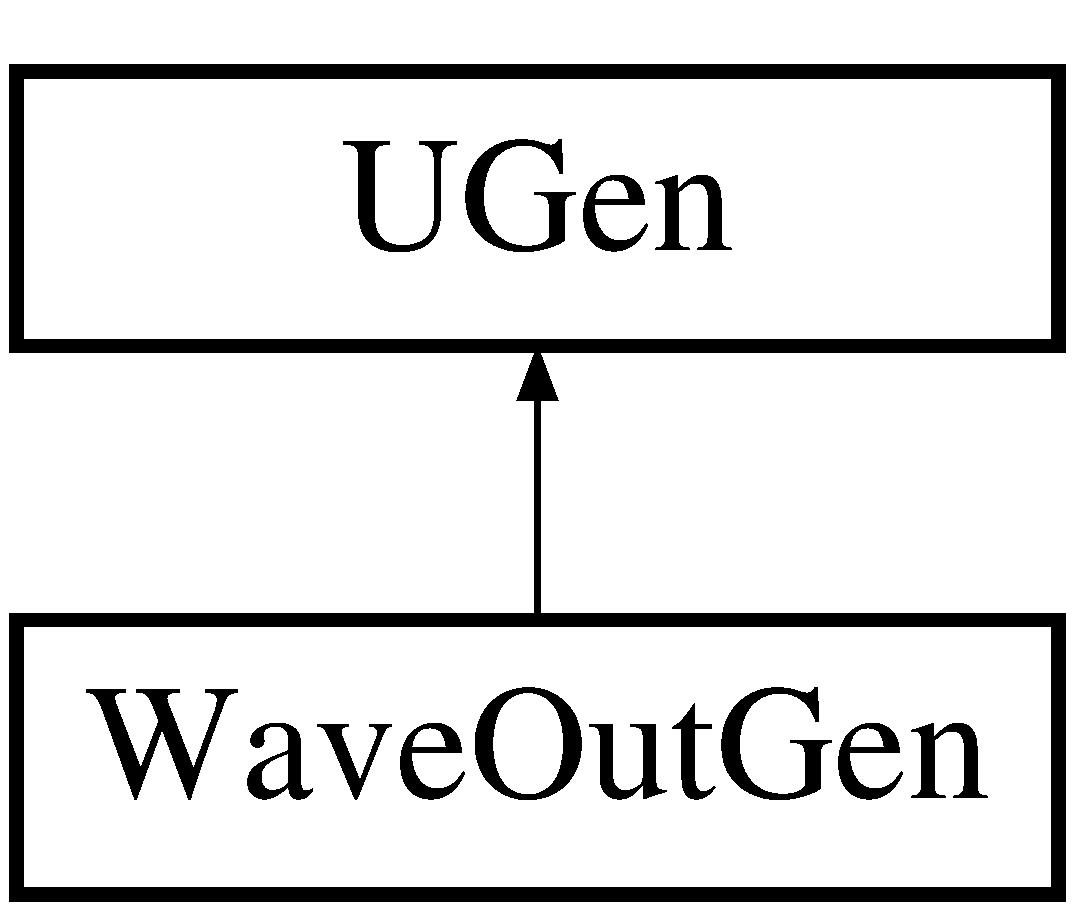
\includegraphics[height=2.000000cm]{classWaveOutGen}
\end{center}
\end{figure}
\subsection*{Public Member Functions}
\begin{DoxyCompactItemize}
\item 
{\bfseries Wave\+Out\+Gen} (std\+::string name)\hypertarget{classWaveOutGen_af7b0343212eb3de1ed4ef2dad90ad43e}{}\label{classWaveOutGen_af7b0343212eb3de1ed4ef2dad90ad43e}

\item 
void {\bfseries control} (std\+::string port\+Name, float value)\hypertarget{classWaveOutGen_a919d71ae0729553b3bd1799add9d1088}{}\label{classWaveOutGen_a919d71ae0729553b3bd1799add9d1088}

\item 
float {\bfseries tick} ()\hypertarget{classWaveOutGen_a468581d97aaf471e6516aee2cdb630cd}{}\label{classWaveOutGen_a468581d97aaf471e6516aee2cdb630cd}

\end{DoxyCompactItemize}
\subsection*{Public Attributes}
\begin{DoxyCompactItemize}
\item 
long {\bfseries count} = 0\hypertarget{classWaveOutGen_aa715f14677edeb7ceed397b1624b6b19}{}\label{classWaveOutGen_aa715f14677edeb7ceed397b1624b6b19}

\end{DoxyCompactItemize}
\subsection*{Additional Inherited Members}


The documentation for this class was generated from the following files\+:\begin{DoxyCompactItemize}
\item 
unit/Wave\+Out\+Gen.\+h\item 
unit/Wave\+Out\+Gen.\+cpp\end{DoxyCompactItemize}

\hypertarget{classWaveWriter}{\section{Wave\-Writer Class Reference}
\label{classWaveWriter}\index{Wave\-Writer@{Wave\-Writer}}
}
\subsection*{Public Member Functions}
\begin{DoxyCompactItemize}
\item 
\hypertarget{classWaveWriter_ab56ef6702c7c651004329fe76893b2f7}{{\bfseries Wave\-Writer} (std\-::string fname)}\label{classWaveWriter_ab56ef6702c7c651004329fe76893b2f7}

\item 
\hypertarget{classWaveWriter_a369569d5d2068f497731936073ad4ad1}{void {\bfseries open} (std\-::string fname)}\label{classWaveWriter_a369569d5d2068f497731936073ad4ad1}

\item 
\hypertarget{classWaveWriter_ae50259472af637a4083399953440ee0e}{void {\bfseries close} ()}\label{classWaveWriter_ae50259472af637a4083399953440ee0e}

\item 
\hypertarget{classWaveWriter_a267d0704f57004f0adf079096d3dc460}{void {\bfseries write} (float value)}\label{classWaveWriter_a267d0704f57004f0adf079096d3dc460}

\end{DoxyCompactItemize}


The documentation for this class was generated from the following files\-:\begin{DoxyCompactItemize}
\item 
include/Wave\-Writer.\-h\item 
util/Wave\-Writer.\-cpp\end{DoxyCompactItemize}

\hypertarget{classWorkItem}{}\section{Work\+Item Class Reference}
\label{classWorkItem}\index{Work\+Item@{Work\+Item}}
\subsection*{Public Member Functions}
\begin{DoxyCompactItemize}
\item 
{\bfseries Work\+Item} (const char $\ast$message, int number)\hypertarget{classWorkItem_ac77d1e967d872c2ceb4de4ea3ac45c78}{}\label{classWorkItem_ac77d1e967d872c2ceb4de4ea3ac45c78}

\item 
const char $\ast$ {\bfseries get\+Message} ()\hypertarget{classWorkItem_a5e25f8c72fd1213c9e975c988e2a96c4}{}\label{classWorkItem_a5e25f8c72fd1213c9e975c988e2a96c4}

\item 
int {\bfseries get\+Number} ()\hypertarget{classWorkItem_a9741f02d319a3843b62ec72b9181f71c}{}\label{classWorkItem_a9741f02d319a3843b62ec72b9181f71c}

\end{DoxyCompactItemize}


The documentation for this class was generated from the following file\+:\begin{DoxyCompactItemize}
\item 
store/gqueue.\+cpp\end{DoxyCompactItemize}

%--- End generated contents ---

% Index
\backmatter
\newpage
\phantomsection
\clearemptydoublepage
\addcontentsline{toc}{chapter}{Index}
\printindex

\end{document}
